\documentclass[12pt,a4paper]{report}

%% ---
\usepackage[utf8]{inputenc}
\usepackage[T1]{fontenc}
\usepackage[french]{babel}
\usepackage{csquotes}

%% ---
\usepackage{geometry}
\geometry{margin=2.5cm}

%% ---
\usepackage{background}
\usepackage[absolute]{textpos}
\setlength{\TPHorizModule}{1cm}
\setlength{\TPVertModule}{1cm}

%% ---
\usepackage{amsmath}
\usepackage{amssymb}

%% ---
\usepackage{graphicx}
\graphicspath{{figures/}{images/}{./}}
\DeclareGraphicsExtensions{.png,.jpg,.jpeg,.pdf,.eps}
\usepackage{float}
\usepackage{caption}
\usepackage{subcaption}
\usepackage[section]{placeins}

%% ---
\usepackage[dvipsnames,svgnames,table]{xcolor}
\definecolor{uveyblue}{RGB}{0,80,160}
\definecolor{uveylight}{RGB}{235,243,255}

%% ---
\usepackage{listings}
\lstset{
  basicstyle=\small\ttfamily,
  breaklines=true,
  frame=single,
  numbers=left,
  numberstyle=\tiny\color{gray},
  keywordstyle=\color{blue}\bfseries,
  stringstyle=\color{orange},
  commentstyle=\color{gray}\itshape,
  showstringspaces=false,
  tabsize=2,
  captionpos=b,
}
\lstdefinelanguage{Dockerfile}{
  keywords={FROM,RUN,CMD,EXPOSE,ENV,ADD,COPY,WORKDIR,USER,ENTRYPOINT,VOLUME,ARG},
  morecomment=[l]{\#},
  morestring=[b]",
}
\lstdefinelanguage{YAML}{
  keywords={true,false,null,yes,no},
  keywordstyle=\color{blue}\bfseries,
  sensitive=false,
  comment=[l]{\#},
  commentstyle=\color{gray}\itshape,
  morestring=[b]',
  morestring=[b]",
}
\lstdefinelanguage{Terraform}{
  keywords={resource,variable,output,module,locals,data,provider,terraform},
  keywordstyle=\color{blue}\bfseries,
  comment=[l]{\#},
  commentstyle=\color{gray}\itshape,
  morestring=[b]",
}

%% ---
\usepackage{booktabs}
\usepackage{tabularx}
\usepackage{multirow}
\usepackage{longtable}
\usepackage{array}
\usepackage{colortbl}
\newcolumntype{L}[1]{>{\raggedright\arraybackslash}p{#1}}
\newcolumntype{C}[1]{>{\centering\arraybackslash}p{#1}}
\newcolumntype{R}[1]{>{\raggedleft\arraybackslash}p{#1}}

%% ---
\usepackage{hyperref}
\hypersetup{colorlinks=true, linkcolor=blue, citecolor=blue, urlcolor=blue}
\usepackage{url}

%% ---
\usepackage[numbers,sort&compress]{natbib}

%% ---
\usepackage{enumitem}
\setlist[itemize]{leftmargin=*, topsep=3pt, itemsep=1pt, parsep=0pt}
\setlist[enumerate]{leftmargin=*, topsep=3pt, itemsep=1pt, parsep=0pt}
\usepackage{mdframed}
\usepackage{tcolorbox}
\tcbuselibrary{skins,breakable}
\usepackage{acronym}
\usepackage{tikz}
\usetikzlibrary{arrows.meta,shapes,positioning,fit,backgrounds}
\usepackage{pgfplots}
\pgfplotsset{compat=1.18}
\usepackage{setspace}
\onehalfspacing
\usepackage[bottom]{footmisc}
\setlength{\textfloatsep}{10pt plus 2pt minus 4pt}
\setlength{\floatsep}{8pt plus 2pt minus 2pt}
\setlength{\intextsep}{8pt plus 2pt minus 2pt}
\usepackage{titlesec}
\titlespacing*{\section}{0pt}{14pt}{6pt}
\titlespacing*{\subsection}{0pt}{10pt}{4pt}
\titlespacing*{\subsubsection}{0pt}{8pt}{3pt}

%% ---
\tcbset{
  defbox/.style={
    enhanced, breakable,
    colback=blue!5, colframe=blue!60!black,
    fonttitle=\bfseries,
    boxrule=0.5pt, arc=4pt
  },
  notebox/.style={
    enhanced, breakable,
    colback=yellow!10, colframe=orange!70!black,
    fonttitle=\bfseries, title={Remarque},
    boxrule=0.5pt, arc=4pt
  },
  warnbox/.style={
    enhanced, breakable,
    colback=red!5, colframe=red!60!black,
    fonttitle=\bfseries, title={Important},
    boxrule=0.5pt, arc=4pt
  }
}

%% ---
\newcommand{\tech}[1]{\texttt{\textbf{#1}}}
\newcommand{\figref}[1]{(cf.~figure~\ref{#1})}
\newcommand{\tabref}[1]{(cf.~tableau~\ref{#1})}
\newcommand{\secref}[1]{(cf.~section~\ref{#1})}
\newcommand{\chapref}[1]{(cf.~chapitre~\ref{#1})}
\newcommand{\imgsource}[2]{%
  \par\vspace{2pt}%
  \noindent{\footnotesize\textit{Source~:~#1}%
  \ifx&#2&\else\quad\href{#2}{\textcolor{uveyblue}{\fbox{\tiny\textbf{Voir la source}}}}\fi}%
}

%% ---
\acrodef{IDP}{Internal Developer Platform}
\acrodef{IaC}{Infrastructure as Code}
\acrodef{CI/CD}{Continuous Integration / Continuous Deployment}
\acrodef{AKS}{Azure Kubernetes Service}
\acrodef{VNet}{Virtual Network}
\acrodef{NSG}{Network Security Group}
\acrodef{WAF}{Web Application Firewall}
\acrodef{AGIC}{Application Gateway Ingress Controller}
\acrodef{CNI}{Container Network Interface}
\acrodef{GCS}{Google Cloud Storage}
\acrodef{GCR}{Google Container Registry}
\acrodef{GCP}{Google Cloud Platform}
\acrodef{SLA}{Service Level Agreement}
\acrodef{PFE}{Projet de Fin d'Études}
\acrodef{PME}{Petites et Moyennes Entreprises}
\acrodef{TPE}{Très Petites Entreprises}
\acrodef{ETI}{Entreprises de Taille Intermédiaire}
\acrodef{GED}{Gestion Électronique des Documents}
\acrodef{SaaS}{Software as a Service}
\acrodef{FinTech}{Financial Technology}
\acrodef{RBAC}{Role-Based Access Control}
\acrodef{API}{Application Programming Interface}
\acrodef{CNCF}{Cloud Native Computing Foundation}
\acrodef{DX}{Developer Experience}
\acrodef{ILM}{Index Lifecycle Management}
\acrodef{JVM}{Java Virtual Machine}
\acrodef{MTTR}{Mean Time To Recovery}
\acrodef{OCR}{Optical Character Recognition}
\acrodef{SDK}{Software Development Kit}

% ============================================================
\begin{document}

%% ---

\backgroundsetup{
scale=1,
color=black,
opacity=1,
angle=0,
contents={%
  
\includegraphics[width=19cm,height=28.5cm]{background.png}
  }%
}
\begin{titlepage}
\BgThispage

% Top logos row
\begin{center}
\begin{minipage}[c]{0.25\textwidth}
  \centering
  
\includegraphics[height=2cm]{logoUTM.png}
\end{minipage}
\hfill
\begin{minipage}[c]{0.25\textwidth}
  \centering
  
\includegraphics[height=2cm]{logoEnit.png}
\end{minipage}
\end{center}

\vspace{0.3cm}

\begin{center}
{Université de Tunis El Manar\\[0.2cm]
\textbf{École Nationale d'Ingénieurs de Tunis}\\[0.2cm]
Département Technologies de l'Information et de la Communication}\\[0.6cm]

{\Large \textbf{Rapport de Projet de Fin d'Études}}\\[0.5cm]

{\emph{Présenté par :}}\\[0.3cm]
{\large \textbf{Jasser Hasni}}\\[0.4cm]
{\emph{En vue de l'obtention du :}}\\[0.3cm]
{\large \textbf{Diplôme National d'Ingénieur en Télécommunications}}

% Title
\rule{\linewidth}{0.5mm} \\[0.1cm]
{ \huge \bfseries Mise en Place d'une IDP \\(Internal Developer Platform)
 \\[0.1cm] }
\rule{\linewidth}{0.5mm} \\[0.4cm]

% Host Company

\includegraphics[height=1.4cm]{ENIT_TIC_Report_Template/figures/uvey.png}\\[0.2cm]
{\emph{Entreprise d'accueil :}}\\
{\textbf{Uvey --- Solution SaaS FinTech, Tunis, Tunisie}}\\
\end{center}

\vspace{0.3cm}

% Date
\noindent
{\emph{Date de soutenance :}} {\textbf{25 juin 2026}}\\

% Jury Members
\begin{table}[H]
\begin{tabular}{ll}
\emph{Membres du jury :} \vspace{0.3cm} & \\
Président :         & \textbf{M. Mahmoud Ammar} \\
Rapporteur :        & \textbf{Mme Abir Gallas} \\
Encadrant Entreprise : & \textbf{M. Youssef Meddeb} \\
Encadrant ENIT : & \textbf{Mme Meriem Kassar} \\
\end{tabular}
\end{table}

\vspace{0.3cm}
\begin{center}
Année Universitaire : 2025-2026
\end{center}

\end{titlepage}


%% ---

\chapter*{Signatures}
\thispagestyle{empty}
\bigskip
\begin{center}
{Encadrant Entreprise : M. Youssef Meddeb}
\bigskip
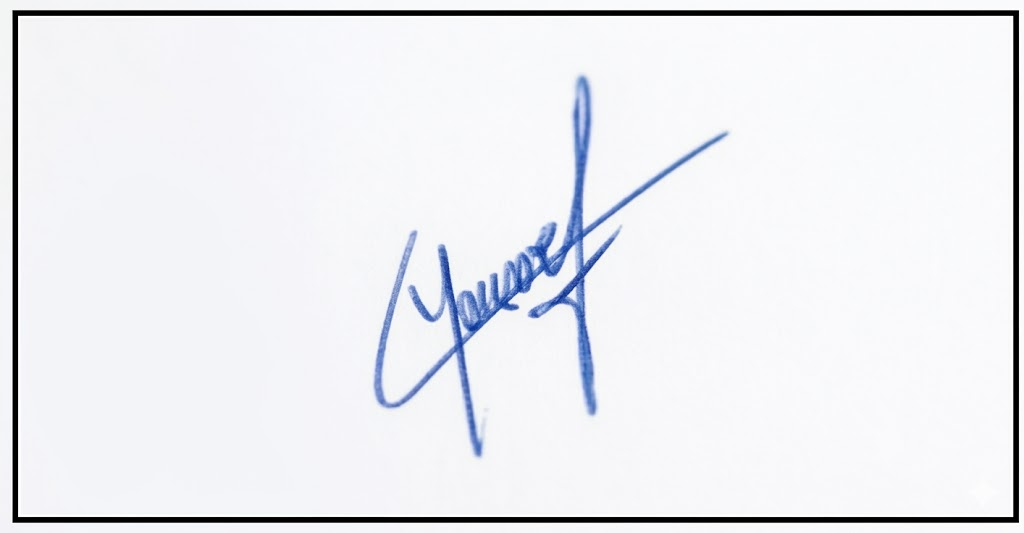
\includegraphics[width=0.8\textwidth]{figures/fig_youssef.png}
\end{center}

\bigskip
\begin{center}
{Encadrant ENIT : Mme Meriem Kassar}
\bigskip

\includegraphics[width=0.8\textwidth]{figures/sig.png}
\end{center}


%% ---
\pagenumbering{roman}

\chapter*{Dédicaces}
\vspace{1cm}

\par \textbf{À mes parents,}\\
pour avoir fait de l'éducation une priorité absolue, souvent au prix de sacrifices silencieux. Chaque ligne de ce rapport leur appartient autant qu'à moi.

\vspace{0.6cm}

\par \textbf{À mes amis et collègues de promotion,}\\
avec qui j'ai partagé trois années d'apprentissage, d'entraide et de persévérance. Ce travail est aussi le reflet de tout ce que nous avons construit ensemble.

\vspace{0.6cm}

\vspace{1cm}

\begin{flushright}
\textit{Jasser}
\end{flushright}

\newpage

\chapter*{Remerciements}
%\addcontentsline{toc}{chapter}{Remerciements}

\textit{À tous ceux qui ont contribué, de près ou de loin, à l'aboutissement de ce projet, je dédie ces quelques mots de reconnaissance.}

\vspace{0.8cm}

Au terme de ce projet de fin d'études, il m'est particulièrement agréable d'exprimer ma gratitude envers toutes les personnes dont le soutien, la confiance et l'expertise ont rendu ce travail possible.

\vspace{0.5cm}

Je remercie en premier lieu les membres du jury pour l'honneur qu'ils me font en acceptant d'examiner et d'évaluer ce travail. Leurs retours critiques constitueront une contribution précieuse à ma formation d'ingénieur.

\vspace{0.5cm}

Mes vifs remerciements s'adressent à \textbf{M. Youssef Meddeb}, mon encadrant industriel au sein d'\textbf{Uvey}, pour m'avoir intégré pleinement au sein de l'équipe d'ingénierie dès les premiers jours. Sa pédagogie, sa disponibilité pour répondre à mes questions techniques, et sa confiance dans les choix que j'ai proposés m'ont permis de m'approprier le projet avec un véritable sentiment de responsabilité. Les échanges réguliers en Sprint Review ont été particulièrement formateurs.

\vspace{0.5cm}

Je tiens à remercier \textbf{Mme Meriem Kassar}, mon encadrante académique, pour la qualité de son suivi tout au long de ce projet. Ses remarques constructives, sa disponibilité lors de chaque point d'avancement, et sa capacité à recadrer les priorités ont été déterminantes pour maintenir la cohérence et la rigueur du travail. Je lui suis reconnaissant d'avoir su allier exigence académique et bienveillance pédagogique.

\vspace{0.5cm}

Je remercie chaleureusement \textbf{l'ensemble de l'équipe technique d'Uvey} pour l'accueil bienveillant, les revues de code, les discussions informelles autour des choix d'architecture, et pour m'avoir traité comme un membre à part entière de l'équipe. Ce contexte de travail collaboratif et exigeant a rendu ce projet à la fois stimulant et formateur bien au-delà du cadre académique.

\vspace{0.5cm}




\newpage

\chapter*{Abstract}
\par This report presents the design, deployment, and validation of an Internal Developer
Platform (IDP) for Uvey, a SaaS FinTech startup based in Tunis, Tunisia. The project
addresses the growing operational complexity of a microservices-based architecture by
centralizing developer tooling, automating infrastructure provisioning through
\textbf{Terraform} and a \textbf{GitOps} workflow with \textbf{ArgoCD}, and deploying a
full observability stack (\textbf{ELK}, \textbf{Prometheus}/\textbf{Grafana},
\textbf{OpenTelemetry}). The IDP, built on \textbf{Backstage}, provides a unified
interface for service catalog management, ephemeral environment provisioning, and access
to monitoring tools. Additionally, the \textbf{PostgreSQL} database was migrated from
\textbf{Google Cloud Platform} to \textbf{Azure} without data loss. Measurable outcomes
include a reduction in mean time to recovery from 45 to 20 minutes and in deployment
time from 20 to 8 minutes.
\vspace{0.5cm}

\noindent{\large \textbf{Keywords:} Internal Developer Platform, Kubernetes, Azure,
GitOps, ArgoCD, Terraform, Backstage, Observability, DevOps, Infrastructure as Code}

\newpage

\chapter*{Résumé}
\par Cette étude détaille la conception, l'implémentation et la vérification d'une
\textit{Internal Developer Platform} (IDP) chez Uvey, une startup SaaS FinTech
installée à Tunis, Tunisie. Cette étude répond aux contraintes de la complexification
technique dans une architecture microservices avec la mise en place d'un ensemble
d'outils pour les développeurs, l'automatisation de la création de l'infrastructure
via \textbf{Terraform} ainsi qu'un flux \textbf{GitOps} avec \textbf{ArgoCD}, et
l'implémentation d'une pile complète d'observabilité (\textbf{ELK},
\textbf{Prometheus}/\textbf{Grafana}, \textbf{OpenTelemetry}). L'\textit{IDP},
bâtie sur \textbf{Backstage}, fournit une interface unifiée pour la gestion du catalogue
de services, le provisionnement d'environnements éphémères et l'accès aux outils de
supervision. De plus, la migration de la base de données \textbf{PostgreSQL} de
\textbf{Google Cloud Platform} vers \textbf{Azure} a été réalisée sans perte de données.
Les résultats mesurables incluent une réduction du temps moyen de résolution des
incidents de 45 à 20 minutes et du temps de déploiement de 20 à 8 minutes.
\vspace{0.5cm}

\noindent{\large \textbf{Mots clés:} Internal Developer Platform, Kubernetes, Azure,
GitOps, ArgoCD, Terraform, Backstage, Observabilité, DevOps, Infrastructure as Code}        % <-- ajouter ici
\newpage


%% ---
\tableofcontents
\newpage

%% ---
\chapter*{Liste des Acronymes}
\addcontentsline{toc}{chapter}{Liste des Acronymes}

\vspace{1cm}
\begin{itemize}
    \item \textbf{AGIC:} Application Gateway Ingress Controller.
    \item \textbf{AKS:} Azure Kubernetes Service.
    \item \textbf{API:} Application Programming Interface.
    \item \textbf{ARM:} Azure Resource Manager.
    \item \textbf{CI/CD:} Continuous Integration / Continuous Deployment.
    \item \textbf{CNI:} Container Network Interface.
    \item \textbf{CNCF:} Cloud Native Computing Foundation.
    \item \textbf{CPU:} Central Processing Unit.
    \item \textbf{DX:} Developer Experience.
    \item \textbf{ELK:} Elasticsearch, Logstash, Kibana.
    \item \textbf{ETI:} Entreprises de Taille Intermédiaire.
    \item \textbf{FinTech:} Financial Technology.
    \item \textbf{GCP:} Google Cloud Platform.
    \item \textbf{GCR:} Google Container Registry.
    \item \textbf{GCS:} Google Cloud Storage.
    \item \textbf{GED:} Gestion Électronique des Documents.
    \item \textbf{IaC:} Infrastructure as Code.
    \item \textbf{IDP:} Internal Developer Platform.
    \item \textbf{ILM:} Index Lifecycle Management.
    \item \textbf{JVM:} Java Virtual Machine.
    \item \textbf{MTTR:} Mean Time To Recovery.
    \item \textbf{NSG:} Network Security Group.
    \item \textbf{OCR:} Optical Character Recognition.
    \item \textbf{PFE:} Projet de Fin d'Études.
    \item \textbf{PME:} Petites et Moyennes Entreprises.
    \item \textbf{RBAC:} Role-Based Access Control.
    \item \textbf{RH:} Ressources Humaines.
    \item \textbf{SaaS:} Software as a Service.
    \item \textbf{SDK:} Software Development Kit.
    \item \textbf{SHA:} Secure Hash Algorithm.
    \item \textbf{SLA:} Service Level Agreement.
    \item \textbf{SSL/TLS:} Secure Sockets Layer / Transport Layer Security.
    \item \textbf{TPE:} Très Petites Entreprises.
    \item \textbf{VNet:} Virtual Network.
    \item \textbf{WAF:} Web Application Firewall.
\end{itemize}

\newpage

%% ---
\listoffigures
\addcontentsline{toc}{chapter}{Liste des Figures}
\newpage

%% ---
\listoftables
\addcontentsline{toc}{chapter}{Liste des Tableaux}
\newpage

%% ---
\pagenumbering{arabic}
\setcounter{page}{1}

\chapter*{Introduction Générale}
\addcontentsline{toc}{chapter}{Introduction Générale}

\noindent Uvey est une startup tunisienne éditrice d'une plateforme SaaS (Software as a Service) B2B de gestion comptable et financière, déployée à destination des PME, TPE et cabinets d'expertise comptable. Son produit repose sur une architecture microservices composée de plus d'une dizaine de services indépendants, rédigés en plusieurs langages (Node.js, Go, Java Spring Boot, Python, C\#), et hébergés jusqu'au début de ce projet sur une infrastructure hétérogène, partiellement managée, sans outillage centralisé.

\vspace{0.4cm}

\noindent À mesure qu'Uvey a évolué d'une architecture initiale vers un écosystème distribué plus complexe, les équipes d'ingénierie ont commencé à absorber une charge opérationnelle croissante, disproportionnée par rapport à la taille de l'organisation. Un développeur souhaitant déployer une mise à jour devait naviguer entre cinq interfaces distinctes : le portail Azure pour l'état des ressources, l'interface ArgoCD pour le statut du déploiement, Grafana pour les métriques, Kibana pour les logs, et GitLab pour les pipelines. La création d'un environnement de test nécessitait une intervention manuelle de l'équipe infrastructure, avec un délai moyen de trente minutes. La résolution d'un incident de production mobilisait en moyenne quarante-cinq minutes, non pas à cause de la complexité du problème, mais à cause du temps passé à reconstituer manuellement le contexte depuis des outils non connectés. Les déploiements en production prenaient vingt minutes, dont une partie significative était consacrée à des vérifications manuelles redondantes. Enfin, l'absence d'un mécanisme de détection des dérives de configuration exposait l'infrastructure à des états divergents non contrôlés entre les environnements.

\vspace{0.4cm}

\noindent Ces dysfonctionnements, pris isolément, pourraient sembler mineurs. Mais leur cumul représentait un coût opérationnel réel : des cycles de livraison ralentis, une frustration croissante des équipes, et un risque accru d'incidents en production dans un contexte où la fiabilité de la plateforme conditionne directement la confiance des clients d'Uvey. La question posée en début de projet était donc la suivante : comment doter des équipes d'ingénierie de taille modeste d'une infrastructure cloud-native de niveau production, sans sacrifier la vélocité de développement ni alourdir davantage la charge cognitive des développeurs ?

\vspace{0.4cm}

\noindent La réponse apportée dans le cadre de ce projet de fin d'études s'articule autour de deux axes complémentaires. Le premier est la migration complète de l'infrastructure vers Microsoft Azure, provisionnée via Terraform selon une approche Infrastructure as Code, avec trois clusters AKS (Azure Kubernetes Service) dédiés, un modèle d'authentification Zero-Trust basé sur les Managed Identities, et un remplacement du contrôleur Ingress NGINX par l'Application Gateway avec protection WAF (Web Application Firewall) intégrée. Le second est la mise en place d'une \textbf{Internal Developer Platform} (IDP) basée sur Backstage, agissant comme point d'entrée unique vers l'ensemble de l'écosystème technique : catalogue des microservices, accès aux outils d'observabilité avec liens pré-filtrés par service, provisionnement autonome des environnements de test en self-service, et intégration du flux GitOps complet avec ArgoCD. Ces deux axes sont complétés par une pile d'observabilité unifiée couvrant les trois piliers fondamentaux : logs via la stack ELK (Elasticsearch, Logstash, Kibana), métriques via Prometheus et Grafana, et traçage distribué via OpenTelemetry.

\vspace{0.5cm}

\noindent \textbf{Ce rapport est organisé en cinq chapitres :}
%\begin{itemize}
Le \textbf{Chapitre 1} pose le cadre général du projet : contexte et motivations spécifiques à Uvey, présentation de l'entreprise d'accueil, problématique opérationnelle identifiée sur le terrain avec ses impacts mesurés, objectifs techniques et fonctionnels, et méthodologies retenues (Scrum et GitOps).
Le \textbf{Chapitre 2} présente la conception et la mise en place de l'Internal Developer Platform basée sur Backstage : choix de la solution par analyse comparative, Software Catalog, proxy Node.js sécurisé vers l'API (Application Programming Interface) Azure ARM (Azure Resource Manager), accès unifié aux outils d'observabilité, et gestion des environnements éphémères en self-service.
Le \textbf{Chapitre 3} détaille la migration vers Azure et la mise en place de l'infrastructure cloud multi-clusters : architecture réseau VNet, déploiement des trois clusters AKS, authentification Zero-Trust, remplacement de l'Ingress NGINX par l'Application Gateway avec AGIC, gestion automatisée via Terraform, et migration de la base de données PostgreSQL depuis GCP (Google Cloud Platform).
Le \textbf{Chapitre 4} décrit la stratégie de déploiement complète : pipelines GitLab CI/CD, flux GitOps avec ArgoCD et Helm Charts, intégration dans l'IDP, scénario de diagnostic d'incident de bout en bout, et métriques de performance avant/après.
Le \textbf{Chapitre 5} présente la pile d'observabilité unifiée : collecte des logs avec Fluent-bit et la stack ELK, monitoring des métriques avec Prometheus et Grafana, traçage distribué avec OpenTelemetry, et intégration de l'ensemble dans l'IDP via des liens pré-filtrés par service.
Une \textbf{conclusion générale} synthétise les réalisations, analyse les difficultés rencontrées et les leçons apprises.
%\end{itemize}


\chapter{Présentation Générale du Projet}
\label{chap:intro}

\section*{Introduction}
\addcontentsline{toc}{section}{Introduction}

Ce premier chapitre pose les bases nécessaires au développement du projet de fin d'études effectué au sein de la société Uvey. Dans un premier temps, le contexte de la transformation numérique qui a rendu ce projet nécessaire est présenté. Dans un deuxième temps, la structure de la société, son domaine d'activité et son environnement sont décrits. Enfin, la problématique concrète identifiée, les objectifs qui s'en dégagent ainsi que les méthodes retenues pour y répondre sont exposés.


\section{Contexte et Motivation du Projet}
\label{sec:contexte}

La digitalisation accrue de l'économie oblige les entreprises à faire appel à une infrastructure informatique de plus en plus complexe afin de rester concurrentielles et de répondre aux besoins de leurs clients. Au cours des dernières années, ce processus de digitalisation a pris un virage historique et transformé radicalement la façon dont les entreprises conçoivent et développent leurs systèmes. Dans ce contexte, le recours aux architectures monolithiques devient inadapté. Bien que ces monolithes aient été choisis en raison de leur simplicité de construction et de leur facilité d'exécution, ils n'ont jamais été en mesure de répondre à toutes les exigences que pose le monde du numérique.

La montée de l'informatique en nuage et de l'architecture de type microservices constitue une rupture totale dans le domaine du développement logiciel. L'application monolithique, qui formait un ensemble unique géré par une seule équipe et déployé en intégralité, est aujourd'hui supplantée par l'architecture de type microservices, qui décompose cette application en de nombreux composants indépendants --- parfois au nombre de plusieurs centaines. Chaque service indépendant dispose de son propre cycle de vie, de son propre dépôt de code, de son propre pipeline de déploiement et de ses propres besoins en infrastructure. Cette évolution est représentée sur la Figure \ref{fig:evolution_archi}.

L'avantage d'une telle approche est évident : possibilité de déploiements séparés, mise à l'échelle individuelle et isolation des pannes. Cependant, chaque avantage a un coût. L'autonomie de chaque composant entraîne une augmentation de la complexité d'orchestration que toutes les équipes impliquées doivent prendre en charge. Ce coût se manifeste par la gestion des relations entre différents services, les orchestrations complexes de déploiements multi-cluster, l'analyse des problèmes dans un environnement distribué, l'harmonisation des configurations sur plusieurs environnements, ainsi que la sécurisation des communications inter-services.

C'est précisément dans ce contexte qu'intervient ce projet. Chez Uvey, la nécessité de simplifier l'expérience quotidienne des développeurs ainsi que d'assurer une observabilité proactive des systèmes distribués a conduit à envisager la création d'un \ac{IDP}. Ce dernier est défini par Gartner comme un niveau d'abstraction qui donne aux équipes produit la possibilité de développer et de déployer leurs applications de manière autonome et sécurisée, sur la base de bonnes pratiques d'infrastructure gérées de façon centralisée par une équipe plateforme. L'\ac{IDP} n'est donc pas seulement un outil : c'est également un levier organisationnel.

À cela s'ajoute la transition de l'infrastructure vers Microsoft Azure, qui contribue à cet objectif : accès à des ressources cloud gérées modernes, meilleure gouvernance des coûts et scalabilité adaptée à la croissance d'Uvey.

\vspace{0.4cm}
\begin{figure}[htbp]
  \centering
  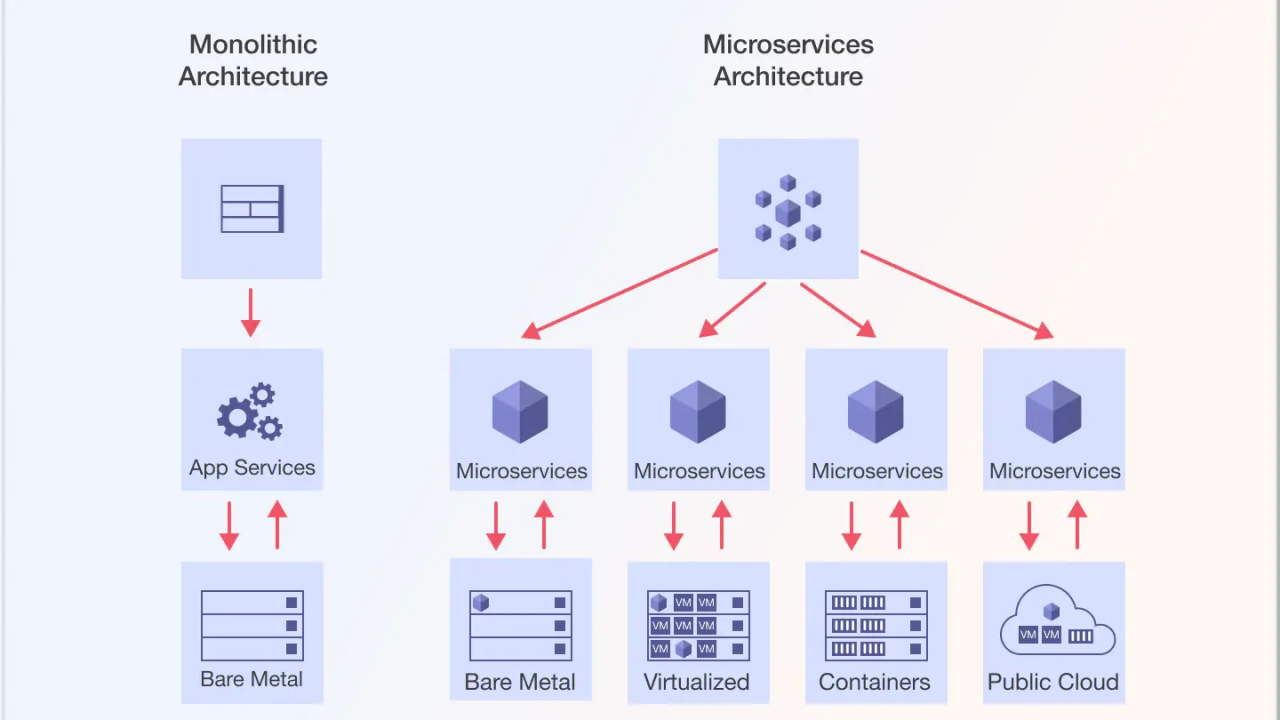
\includegraphics[width=0.85\textwidth]{fig_evolution_architectures}
  \caption{Évolution des architectures logicielles vers les microservices cloud-natifs~\cite{newman2019monolith}}
  \label{fig:evolution_archi}
\end{figure}

\section{Présentation de l'Organisme d'Accueil}
\label{sec:organisme}

Cette section présente la société Uvey dans laquelle le projet de fin d'études a été réalisé, en décrivant son activité, son positionnement sur le marché ainsi que sa structure organisationnelle.

\subsection{Présentation générale}

Ce projet de fin d'études a été réalisé au sein d'Uvey, une société tunisienne basée à Tunis, dont l'activité principale est l'édition d'une solution \ac{SaaS} destinée à la gestion comptable et financière. Dotée d'une vision bien précise --- rendre la comptabilité collaborative, simplifiée et entièrement dématérialisée ---, Uvey a mis au point une plateforme unique à destination des \ac{PME}, \ac{TPE}, \ac{ETI} et cabinets d'expertise comptable tunisiens, dont l'objectif est de moderniser leur gestion financière.

Cette initiative s'inscrit dans une tendance générale de digitalisation rapide du tissu économique tunisien, encouragée aussi bien par la réglementation de la Banque Centrale de Tunisie que par la demande croissante des entreprises pour des outils de gestion modernes et accessibles via le cloud. C'est dans ce contexte de transformation qu'Uvey se positionne comme un acteur reconnu sur le marché, avec un produit conçu spécifiquement pour la région.

La particularité d'Uvey réside dans le fait que son outil se situe précisément à la convergence de la technologie et de la comptabilité professionnelle. Il ne s'agit pas seulement de numériser les procédures existantes, mais surtout de les repenser, en offrant aux entreprises un accès collectif et en temps réel à leurs informations financières et comptables.

La prise en compte du contexte réglementaire local --- notamment les exigences en matière de déclarations fiscales ou de comptabilité générale --- garantit à ses clients une utilisation optimale dès le premier jour.
Le tableau \ref{tab:fiche_uvey} représente la fiche d'identité d'Uvey.

\begin{table}[htbp]
  \centering
  \renewcommand{\arraystretch}{1.3}
  \begin{tabularx}{\textwidth}{p{4cm} X}
    \toprule
    \rowcolor{uveylight}
    \textbf{Raison Sociale} & Uvey \\
    \midrule
    \textbf{Secteur} & \acf{FinTech} / \ac{SaaS} B2B \\
    \midrule
    \textbf{Siège Social} & Tunis, Tunisie \\
    \midrule
    \textbf{Produit Phare} & Plateforme de gestion comptable et financière \\
    \midrule
    \textbf{Cible} & \ac{PME}, \ac{TPE}, \ac{ETI} et cabinets d'expertise comptable \\
    \midrule
    \textbf{Architecture technique} & Cloud-native, microservices, multi-cloud \\
    \midrule
    \textbf{Langages utilisés} & Node.js, Go, Java (Spring Boot), Python, C\# \\
    \bottomrule
  \end{tabularx}
  \caption{Fiche d'identité de la société Uvey}
  \label{tab:fiche_uvey}
\end{table}

\subsection{Organigramme d'Uvey}

Tel que présenté dans l'organigramme ci-dessous (Figure~\ref{fig:organigramme}), Uvey est structurée autour de trois grandes directions : la Direction Technique \& Innovation, la Direction Commerciale \& Partenariats et la Direction Opérations \& Service Client, toutes coordonnées par une Direction Générale ayant pour mission de définir la stratégie et la vision globale de l'entreprise. Cette organisation permet une séparation claire des responsabilités tout en favorisant de fortes interactions entre les différentes lignes métiers.

La Direction Technique \& Innovation est en charge du développement de la plateforme \ac{SaaS}, du pôle Intelligence Artificielle et \ac{GED} intelligente, ainsi que de l'ensemble de l'infrastructure et de la sécurité des données. Elle se doit d'assurer l'évolution technique des solutions proposées par Uvey, et plus particulièrement la mise en œuvre de solutions d'automatisation et d'intelligence artificielle au service de la productivité.

La Direction Commerciale \& Partenariats a pour objectif de développer les relations commerciales avec les cabinets d'expertise comptable et les entreprises, tout en pilotant les équipes Marketing et Communication. Elle veille notamment au développement de la notoriété de la plateforme et à l'accompagnement des clients dans leur transformation digitale.

La Direction Opérations \& Service Client est quant à elle chargée d'accompagner l'ensemble des utilisateurs à travers les services de support, d'assistance, de formation et de suivi client. Elle assure également le respect des exigences réglementaires et juridiques, notamment en matière de conformité aux normes tunisiennes.

Cette organisation traduit la volonté d'Uvey de proposer une plateforme intégrée reposant sur une forte synergie entre l'innovation technologique, le développement commercial et l'excellence opérationnelle.

\vspace{0.4cm}
\begin{figure}[H]
  \centering
  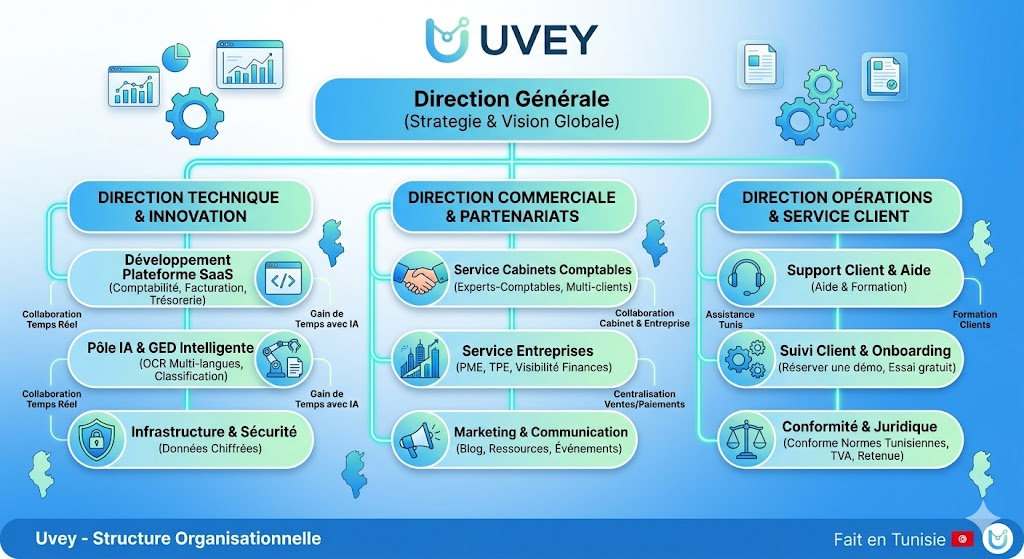
\includegraphics[width=0.88\textwidth]{fig_organigramme_uvey}
  \caption{Organigramme de la société Uvey}
  \label{fig:organigramme}
\end{figure}

\section{Problématique}
\label{sec:problematique}

Le recours à des écosystèmes cloud complexes et à des architectures microservices n'est pas sans incidence sur les équipes d'ingénierie : il engendre un fardeau cognitif grandissant~\cite{forsgren2018accelerate} qui, faute de contrôle, risque de freiner la productivité au lieu de la favoriser. Si la migration vers ces architectures offre de nombreux avantages --- évolutivité, indépendance des déploiements ---, elle tend également à disperser les outils utilisés et les compétences requises au point de devenir contre-productive en l'absence d'une plateforme de coordination.

Chez Uvey, cette problématique se manifeste sous plusieurs symptômes concrets (voir Figure \ref{fig:problematique}).

\begin{itemize}[itemsep=0.2cm, topsep=0.3cm]
  \item \textbf{Dispersion des outils :} les développeurs doivent naviguer entre de multiples interfaces distinctes --- portail Azure, interface ArgoCD, tableau de bord Grafana, index Kibana, interface GitLab --- pour accomplir une tâche de déploiement ou de diagnostic. Ce phénomène de \textit{context switching} imposé engendre une charge cognitive supplémentaire qui nuit à la concentration et allonge les délais de résolution des incidents.
  \item \textbf{Absence de standardisation :} sans processus formalisés et outillés, chaque équipe adopte ses propres conventions de déploiement, générant des incohérences entre environnements et des difficultés de collaboration.
  \item \textbf{Dérives de configuration :} la gestion manuelle des ressources cloud expose l'organisation à des configurations non documentées et non contrôlées, pouvant conduire à des comportements inattendus en production.
  \item \textbf{Visibilité insuffisante :} l'absence d'une vue unifiée sur l'état des services allonge considérablement le MTTR (Mean Time To Recovery) lors des incidents de production, impactant directement la qualité de service offerte aux clients d'Uvey.
  \item \textbf{Dépendance aux équipes infrastructure :} la création d'environnements de test nécessite l'intervention manuelle de l'équipe infrastructure, introduisant des délais incompatibles avec les rythmes de livraison agile.
\end{itemize}

Chacun de ces problèmes pris isolément pourrait paraître mineur. C'est leur combinaison qui révèle l'ampleur du phénomène, lequel est coûteux, source de frustration pour les équipes et constitue une menace pour la qualité des services d'Uvey.

Une estimation interne basée sur les journaux GitLab et les rapports d'incidents des deux derniers mois précédant le démarrage du projet a permis de quantifier ce phénomène. Un développeur perdait en moyenne entre 35 et 40 minutes pour le suivi et le contrôle des déploiements en production, dont une grande partie était consacrée à la corrélation manuelle entre cinq systèmes distincts. La résolution d'un incident en production coûtait quant à elle environ 45 minutes de diagnostic, la majorité de ce temps étant dédiée à la corrélation manuelle de logs, métriques et événements de déploiement issus de sources hétérogènes. Le provisionnement d'un environnement de test nécessitait par ailleurs 30 minutes de travail manuel côté infrastructure, auxquelles s'ajoutaient plusieurs heures d'attente en période chargée.

Dans une équipe de dix développeurs, ces pertes représentaient plusieurs dizaines d'heures chaque semaine.

\begin{figure}[htbp]
  \centering
  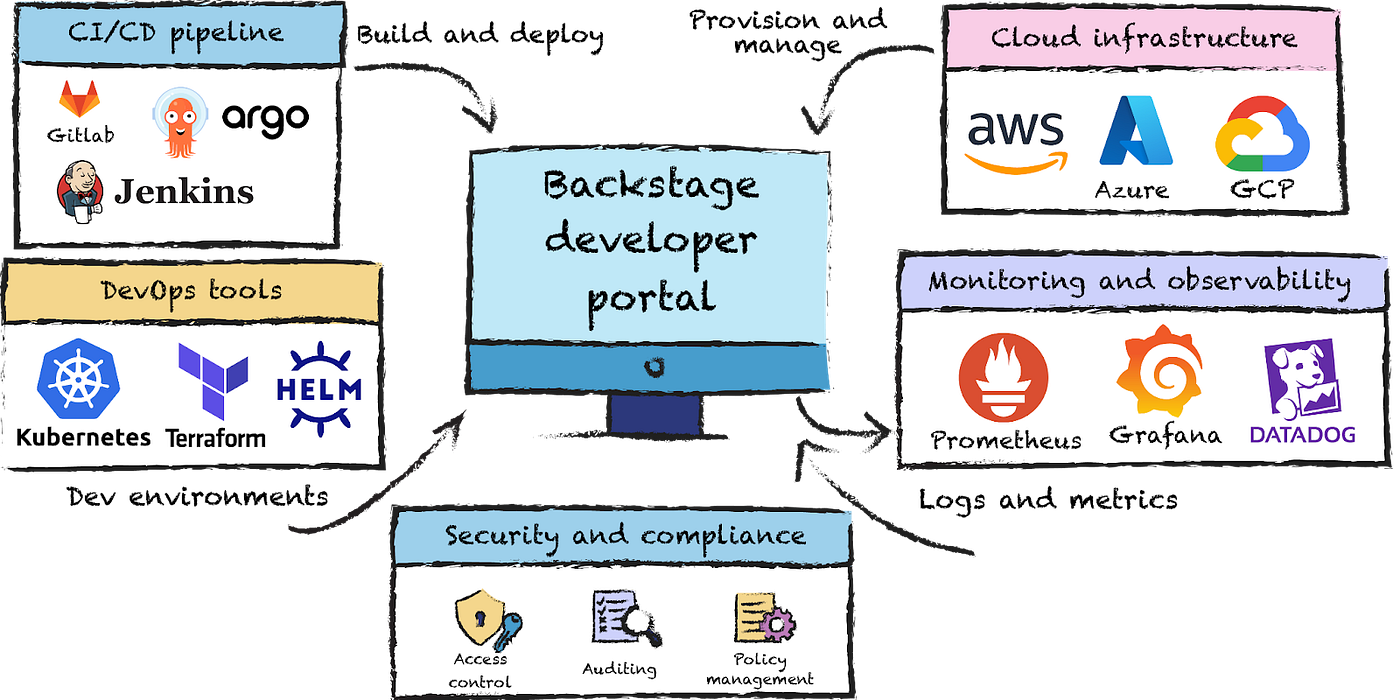
\includegraphics[width=0.88\textwidth]{fig_problematique}
  \caption{Dispersion des outils vs. Centralisation par l'IDP~\cite{noda2023devex}}
  \label{fig:problematique}
\end{figure}

\section{Objectifs du Projet}
\label{sec:objectifs}

Afin de relever ce défi, le projet s'est organisé selon deux dimensions complémentaires : d'une part, des objectifs techniques orientés vers la réalisation d'une plateforme cloud robuste et automatisée ; d'autre part, des objectifs fonctionnels directement liés à l'expérience quotidienne des développeurs. Ces deux dimensions sont indissociables : leur satisfaction simultanée constitue la condition sine qua non pour atteindre l'objectif final du projet, à savoir donner à Uvey les moyens de faire évoluer son ingénierie sans sacrifier la qualité de ses services.

\subsection{Objectifs Techniques}

\begin{itemize}[itemsep=0.2cm, topsep=0.3cm]
  \item Déployer et gérer l'infrastructure cloud via \texttt{Terraform}~\cite{hashicorp2023terraform} sur Microsoft Azure, en provisionnant trois clusters \ac{AKS} distincts (applicatif, automatisation, CI/CD) avec une architecture réseau sécurisée basée sur un \ac{VNet} segmenté.
  \item Implémenter une approche \textbf{GitOps} pour le \ac{CI/CD} avec \texttt{ArgoCD}~\cite{argocd2023docs}, garantissant des déploiements traçables, reproductibles et réversibles via des manifestes versionnés dans Git.
  \item Mettre en place une pile complète d'observabilité couvrant les trois piliers fondamentaux : collecte et analyse des logs via la stack ELK, supervision des métriques via Prometheus et Grafana, et traçage distribué via OpenTelemetry.
  \item Sécuriser l'ensemble des communications inter-services selon le principe \textbf{Zero-Trust}~\cite{nist2020zerotrust} en utilisant des \textit{Managed Identities} Azure Active Directory, éliminant toute dépendance aux secrets statiques.
  \item Migrer la base de données PostgreSQL depuis \ac{GCP} vers Azure sans interruption de service et sans perte de données, en garantissant le chiffrement de bout en bout des données en transit et au repos.
\end{itemize}

\subsection{Objectifs Fonctionnels}

\begin{itemize}[itemsep=0.2cm, topsep=0.3cm]
  \item Développer un portail centralisé (\ac{IDP}) basé sur \texttt{Backstage}~\cite{backstage2023docs}, offrant aux développeurs une interface unifiée pour accéder à l'ensemble des outils, services et informations nécessaires à leur travail quotidien.
  \item Offrir un catalogue logiciel unifié (\textit{Software Catalog}) répertoriant tous les microservices déployés, avec leurs dépendances, leurs propriétaires, leur statut de déploiement en temps réel et leur documentation technique.
  \item Permettre aux développeurs de provisionner et de gérer leurs environnements de test de manière entièrement autonome (\textit{self-service}), sans dépendre des équipes infrastructure.
  \item Intégrer l'ensemble des outils d'observabilité (Grafana, Kibana, OpenTelemetry) dans l'\ac{IDP} avec des liens pré-filtrés par service, réduisant drastiquement le temps de diagnostic lors des incidents.
\end{itemize}

\section{Méthodologies Adoptées}
\label{sec:methodologies}

La conduite d'un projet situé à la croisée du développement logiciel, du cloud computing et de la transformation des pratiques d'ingénierie nécessite le recours à des méthodes efficaces, capables de neutraliser les incertitudes inhérentes à l'innovation. C'est pourquoi deux approches complémentaires ont été adoptées tout au long du projet.

\subsection{Méthode Agile Scrum}

Le développement de la plateforme \ac{IDP} et le management de l'infrastructure ont été conduits selon la méthode Scrum Agile~\cite{schwaber2020scrum}, organisée en cycles itératifs de deux semaines appelés \textit{Sprints}. Chaque sprint est structuré autour de quatre cérémonies : le \textit{Sprint Planning}, lors duquel l'objectif et le périmètre de l'itération sont définis ; le \textit{Daily stand-up}, qui assure la coordination quotidienne de l'équipe ; la \textit{Sprint Review}, qui consiste en une présentation des réalisations aux parties prenantes ; et la \textit{Sprint Retrospective}, qui vise à améliorer le processus de travail.

Le recours à cette approche a été motivé par une comparaison préliminaire des différentes méthodes de gestion de projet disponibles, présentée dans le tableau~\ref{tab:methodo_comparaison}.

\begin{table}[htbp]
  \centering
  \renewcommand{\arraystretch}{1.3}
  \begin{tabularx}{\textwidth}{L{3cm} L{3.5cm} L{3.5cm} L{3.5cm}}
    \toprule
    \rowcolor{uveylight}
    \textbf{Critère} & \textbf{Scrum} & \textbf{Kanban} & \textbf{Cycle en V} \\
    \midrule
    Adaptabilité      & Élevée (sprints) & Élevée (flux continu) & Faible (figé) \\
    Livraisons        & Incrémentales (2 sem.) & Continue & Unique (fin de projet) \\
    Feedback client   & À chaque sprint & Continu & En fin de projet \\
    Planification     & Backlog priorisé & Flux de tâches & Jalons figés en amont \\
    Convient pour     & Projets évolutifs & Maintenance & Projets bien définis \\
    Visibilité        & Backlog + burndown & Tableau Kanban & Jalons figés \\
    \textbf{Choix}    & \textbf{Retenu} & Non retenu & Non retenu \\
    \bottomrule
  \end{tabularx}
  \caption{Comparaison des méthodologies de gestion de projet}
  \label{tab:methodo_comparaison}
\end{table}

Scrum s'impose comme le choix le plus adapté dans ce contexte pour une raison fondamentale : la nature évolutive du projet a rendu nécessaire une adaptation continue du périmètre à chaque itération. Kanban, bien qu'efficace pour l'exploitation d'un système existant, ne convient pas à un projet de cette envergure qui nécessite une structure itérative pour sa planification. Quant au Cycle en V, il suppose que le besoin soit entièrement défini en amont, ce qui va à l'encontre de la démarche de recherche technologique adoptée ici. Une démonstration formelle de chaque sprint a été réalisée auprès de l'encadrant industriel Uvey.
La Figure \ref{fig:scrum} représente le cycle de développement Scrum appliquée au projet.

\begin{figure}[H]
  \centering
  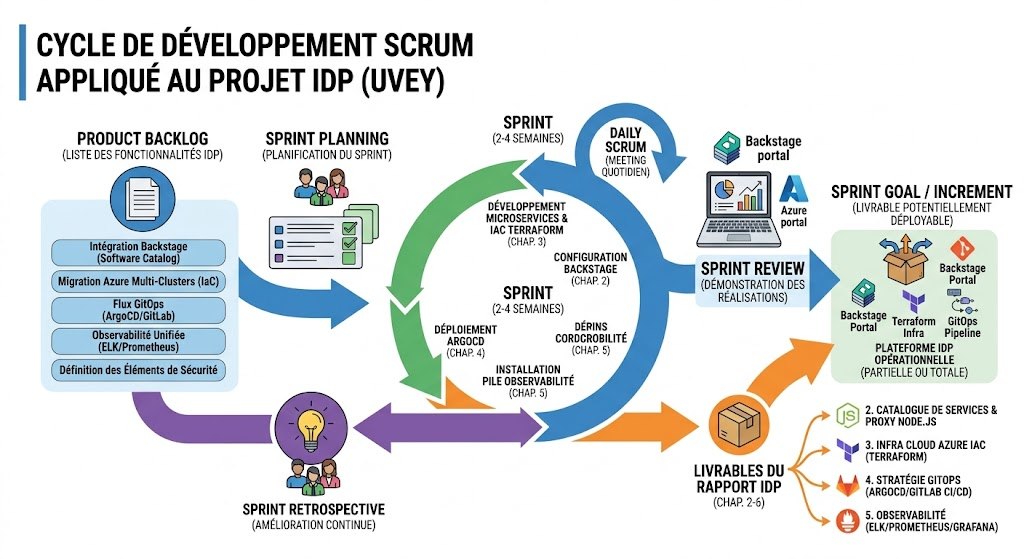
\includegraphics[width=0.95\textwidth]{fig_scrum}
  \caption{Cycle de développement Scrum appliqué au projet~\cite{schwaber2020scrum}}
  \label{fig:scrum}
\end{figure}

\subsection{Approche GitOps}

La gestion de l'infrastructure cloud et le déploiement des applications sont réalisés selon le paradigme GitOps~\cite{weaveworks2021gitops}. La logique sous-jacente est simple mais puissante : Git devient l'unique source de vérité concernant l'état attendu du système. Tout changement --- qu'il porte sur l'infrastructure ou sur la configuration applicative --- passe obligatoirement par une \textit{pull request} revue avant fusion. Plusieurs approches de déploiement ont été évaluées ; c'est GitOps qui a finalement été retenu au regard des critères de sécurité et de traçabilité du projet, comme le montre le tableau~\ref{tab:gitops_comparaison}.

\begin{table}[H]
  \centering
  \renewcommand{\arraystretch}{1.3}
  \begin{tabularx}{\textwidth}{L{3.5cm} L{3.5cm} L{3.5cm} L{3cm}}
    \toprule
    \rowcolor{uveylight}
    \textbf{Critère} & \textbf{GitOps (ArgoCD)} & \textbf{CI/CD push classique} & \textbf{Scripts manuels} \\
    \midrule
    Traçabilité       & Complète (Git history) & Partielle (logs CI) & Inexistante \\
    Rollback          & \texttt{git revert} immédiat & Rebuild du pipeline & Manuel, risqué \\
    Sécurité cluster  & Aucun accès externe requis & Accès direct cluster & Accès direct cluster \\
    Dérive config.    & Détectée et corrigée auto. & Non détectée & Non détectée \\
    Auditabilité      & Totale & Partielle & Nulle \\
    Réconciliation    & Continue et automatique & À chaque pipeline & Inexistante \\
    \textbf{Choix}    & \textbf{Retenu} & Non retenu & Non retenu \\
    \bottomrule
  \end{tabularx}
  \caption{Comparaison des approches de déploiement d'infrastructure}
  \label{tab:gitops_comparaison}
\end{table}

GitOps a été retenu pour trois raisons fondamentales. Premièrement, sa traçabilité complète : chaque modification de l'infrastructure est associée à un commit Git portant un auteur, un message explicatif et un horodatage précis, constituant un journal d'audit immuable. Deuxièmement, sa sécurité renforcée : les clusters de production n'exposent aucune API d'administration accessible depuis les pipelines \ac{CI/CD} externes, réduisant drastiquement la surface d'attaque. Troisièmement, sa capacité de réconciliation continue : ArgoCD détecte automatiquement toute dérive entre l'état déclaré dans Git et l'état réel des clusters, et la corrige sans intervention humaine.

%\vspace{3cm}
\section*{Conclusion}
\addcontentsline{toc}{section}{Conclusion}

Ce premier chapitre a posé les bases du projet. Le contexte de la révolution numérique et les spécificités de l'architecture microservices ont été exposés, aboutissant à une présentation détaillée d'Uvey, son positionnement innovant dans le domaine de la FinTech tunisienne et sa stratégie de fonctionnement. La problématique de dispersion des outils et de charge cognitive pesant sur les équipes a été établie sur la base d'observations pratiques et de données quantifiées. Enfin, Scrum et GitOps ont été retenus comme méthodologies après des évaluations rigoureuses et adaptées au contexte du projet.

Le chapitre suivant aborde la conception et la mise en œuvre de l'\ac{IDP}, cœur technique du présent travail.


\chapter{Mise en place de l'Internal Developer Platform}
\label{chap:idp}

\section*{Introduction}
\addcontentsline{toc}{section}{Introduction}

Le présent chapitre porte sur la conception et la mise en œuvre de l'\ac{IDP} au sein de l'architecture d'Uvey. Après une justification du choix de Backstage par une comparaison des différentes solutions disponibles sur le marché, les composants qui constituent l'\ac{IDP} sont détaillés : le \textit{Software Catalog} pour la centralisation des services, le proxy Node.js pour une intégration sécurisée avec les services Azure, l'accès unifié à tous les outils d'observabilité, et enfin le provisionnement autonome des environnements éphémères.

\section{Présentation de la plateforme}
\label{sec:idp_presentation}

L'\ac{IDP} constitue le point central de la stratégie mise en place pour améliorer l'expérience développeur et faciliter la gestion de l'infrastructure. Dans un environnement où les ingénieurs travaillent quotidiennement avec de nombreux outils --- portails cloud, outils de déploiement, plateformes de surveillance, wikis, registres de conteneurs --- une plateforme unifiée représente un levier de productivité considérable. Plutôt que de multiplier les interfaces, l'\ac{IDP} joue le rôle d'un agrégateur intelligent, qui présente à l'utilisateur les informations pertinentes dans le bon contexte.

Dans le cadre de ce projet, le choix s'est porté sur \textbf{Backstage}~\cite{backstage2023docs}, un framework open-source développé par \textbf{Spotify} en 2020 pour répondre aux besoins de gestion interne de son architecture microservices. Ce framework se caractérise par sa modularité, fondée sur une architecture de plugins qui lui permet de fédérer dans une interface unique l'ensemble des outils et services d'une organisation. Il repose sur trois éléments principaux : un catalogue de services (\textit{Software Catalog}), qui regroupe sous un même toit tous les microservices, \ac{API} et autres ressources ; un système de templates facilitant la création de projets selon des \textit{Golden Paths} récapitulant les bonnes pratiques de l'organisation ; et une documentation technique intégrée via TechDocs. La Figure~\ref{fig:backstage_home} présente la page d'accueil de l'\ac{IDP} telle qu'elle a été déployée chez Uvey, mettant en évidence la navigation unifiée vers le \textit{Software Catalog}, les outils d'observabilité et les templates de provisionnement, le tout accessible depuis une interface unique.

\begin{figure}[H]
  \centering
  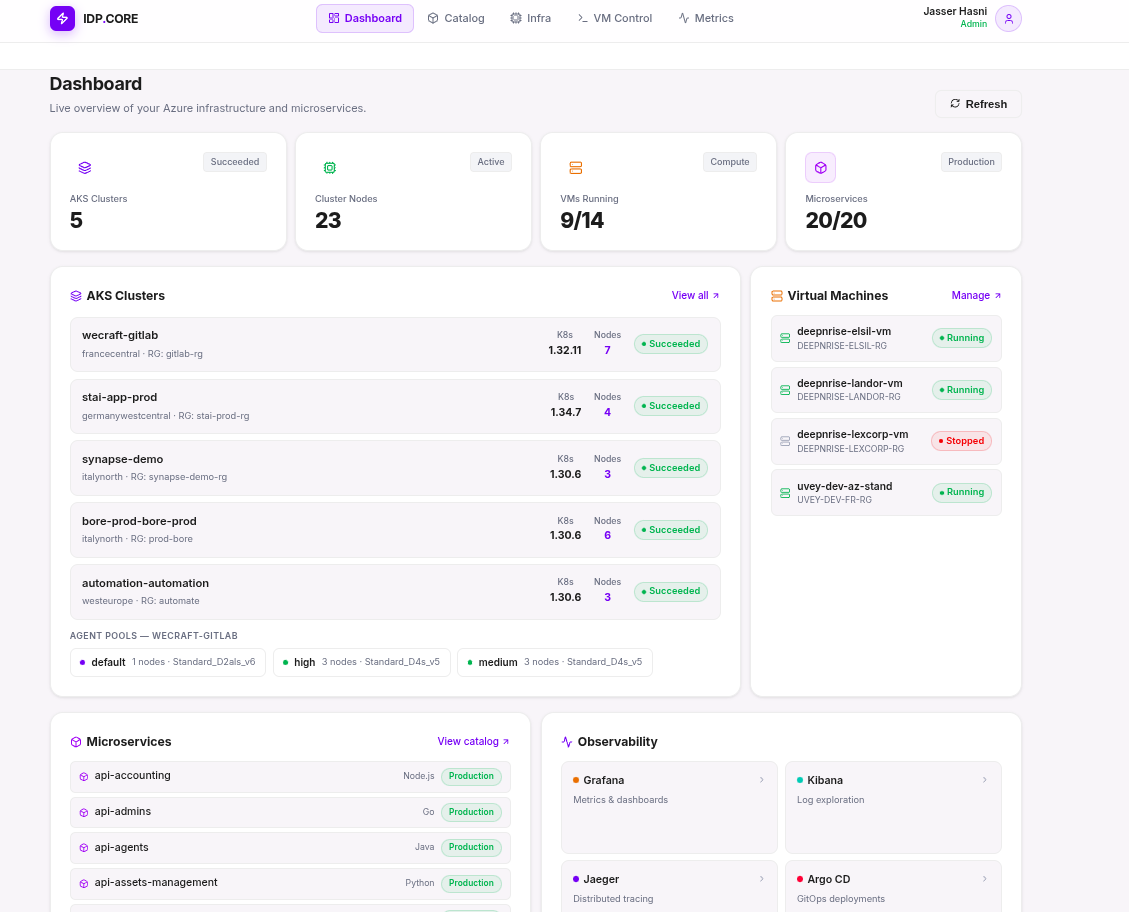
\includegraphics[width=\textwidth]{fig_backstage_home}
  \caption{Page d'accueil de l'\ac{IDP} basée sur Backstage~\cite{backstage2023docs}}
  \label{fig:backstage_home}
\end{figure}

\section{Choix de la solution IDP}
\label{sec:idp_choix}

Le choix d'une solution \ac{IDP} est une décision structurante dont les conséquences s'inscrivent dans la durée. Un mauvais choix se traduit inévitablement par une dette technique non négligeable, des coûts de licences imprévus ou une dépendance vis-à-vis d'un fournisseur incompatible avec les évolutions futures d'Uvey. Avant de retenir Backstage, une étude comparative approfondie a été conduite selon plusieurs critères fondamentaux : l'étendue fonctionnelle de la solution, la richesse de l'écosystème de plugins, la viabilité économique à long terme, la vitalité de la communauté open-source et la facilité d'intégration avec les outils existants, comme le montre le Tableau~\ref{tab:idp_comparaison}.

\begin{table}[H]
  \centering
  \renewcommand{\arraystretch}{1.3}
  \begin{tabularx}{\textwidth}{L{2.8cm} C{1.8cm} C{1.8cm} C{1.8cm} C{1.8cm} C{1.8cm}}
    \toprule
    \rowcolor{uveylight}
    \textbf{Critère} & \textbf{Backstage} & \textbf{Port.io} & \textbf{Cortex} & \textbf{OpsLevel} & \textbf{Dev maison} \\
    \midrule
    Open-source        & \textcolor{OliveGreen}{\checkmark} & $\times$ & $\times$ & $\times$ & \textcolor{OliveGreen}{\checkmark} \\
    Extensibilité      & Élevée & Moyenne & Moyenne & Faible & Totale \\
    Catalogue logiciel & Natif & Natif & Natif & Natif & À développer \\
    Communauté         & Très large (\ac{CNCF}) & Limitée & Limitée & Limitée & N/A \\
    Coût               & Gratuit & Payant & Payant & Payant & Élevé (temps) \\
    Intégrations       & 200+ plugins & Limitées & Limitées & Limitées & Sur mesure \\
    Déploiement        & Self-hosted & SaaS & SaaS & SaaS & Self-hosted \\
    Maturité           & Production (Spotify, Netflix) & En croissance & En croissance & En croissance & Inexistante \\
    \textbf{Choix}     & \textbf{Retenu} & Non retenu & Non retenu & Non retenu & Non retenu \\
    \bottomrule
  \end{tabularx}
  \caption{Comparaison des solutions d'\acl{IDP}}
  \label{tab:idp_comparaison}
\end{table}

Backstage se positionne comme la solution la plus pertinente pour plusieurs raisons. Premièrement, son caractère open-source garantit une transparence totale et une absence de dépendance envers un éditeur, évitant ainsi tout risque de coût imprévu. Deuxièmement, son écosystème de plus de deux cents plugins couvre nativement la quasi-totalité des intégrations nécessaires à Uvey --- ArgoCD, GitLab, Grafana, Kubernetes, Azure --- ce qui réduit considérablement l'effort de développement. Troisièmement, Backstage est utilisé en production par des entreprises de premier plan comme Spotify, Netflix, American Airlines ou Zalando, ce qui atteste de sa fiabilité à grande échelle.

La solution \ac{IDP} ainsi construite est conçue pour fournir un \textit{Single Pane of Glass} --- une porte d'entrée unique vers l'écosystème technique d'Uvey ---, simplifier la compréhension du système en faisant abstraction de la complexité infrastructurelle, automatiser les processus récurrents via les \textit{Golden Paths}~\cite{spotify2021goldenpath}, et assurer l'auditabilité de toutes les applications. La Figure~\ref{fig:idp_architecture} illustre l'architecture globale de l'\ac{IDP} et ses interconnexions avec l'infrastructure, faisant apparaître les flux de communication entre Backstage, le proxy Node.js, l'\ac{API} Azure ARM, les clusters \ac{AKS} et les outils d'observabilité.

\begin{figure}[htbp]
  \centering
  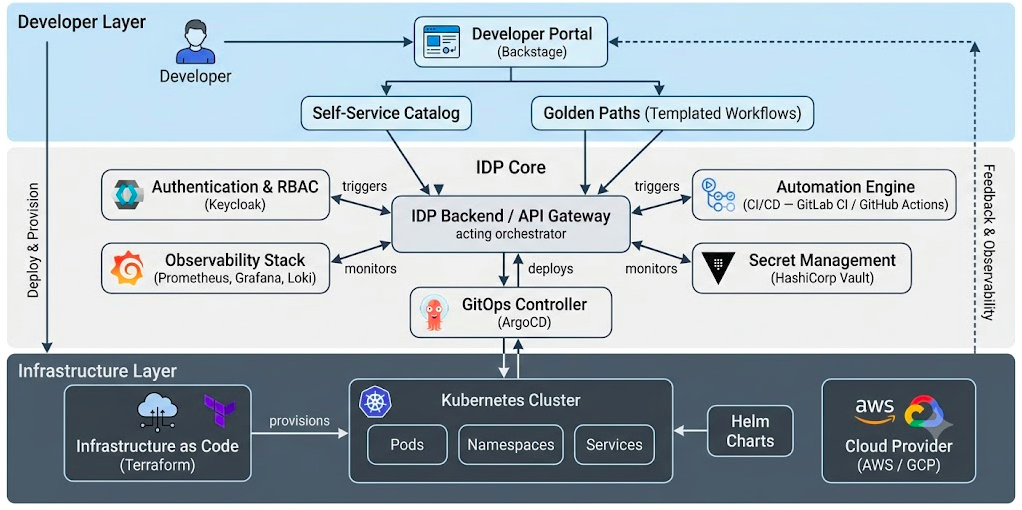
\includegraphics[width=\textwidth]{fig_idp_architecture}
  \caption{Architecture globale de l'\ac{IDP} et ses interconnexions avec l'infrastructure~\cite{backstage2023docs}}
  \label{fig:idp_architecture}
\end{figure}

\section{Centralisation des services --- Software Catalog}
\label{sec:software_catalog}

L'une des difficultés courantes dans les organisations qui adoptent une architecture microservices est la perte de visibilité sur l'ensemble de la structure applicative. Qui est responsable de tel service ? Quelle version est déployée en production ? Où se trouve la documentation ? Ces questions, a priori simples, peuvent exiger un temps considérable à résoudre, notamment dans un contexte où le turnover au sein des équipes est important.

C'est précisément pour répondre à ce type de problème que Backstage propose la fonctionnalité de \textbf{Software Catalog}~\cite{backstage2023catalog}, qui recense l'ensemble des microservices présents dans l'infrastructure et fournit pour chacun d'eux les informations suivantes : son nom et sa description, ses propriétaires, ses dépendances vis-à-vis des autres services, son état de déploiement en temps réel via ArgoCD, les URL des outils de monitoring et la documentation OpenAPI. Ces informations sont stockées dans un fichier \texttt{catalog-info.yaml} présent directement dans le dépôt Git du microservice, garantissant ainsi une synchronisation permanente avec le code source. La Figure~\ref{fig:software_catalog} présente la vue liste du \textit{Software Catalog} tel qu'il apparaît dans l'\ac{IDP}, où chaque entrée expose en un coup d'œil le propriétaire du service, son statut de déploiement ArgoCD en temps réel et les liens directs vers sa documentation et ses outils de supervision.

\begin{figure}[htbp]
  \centering
  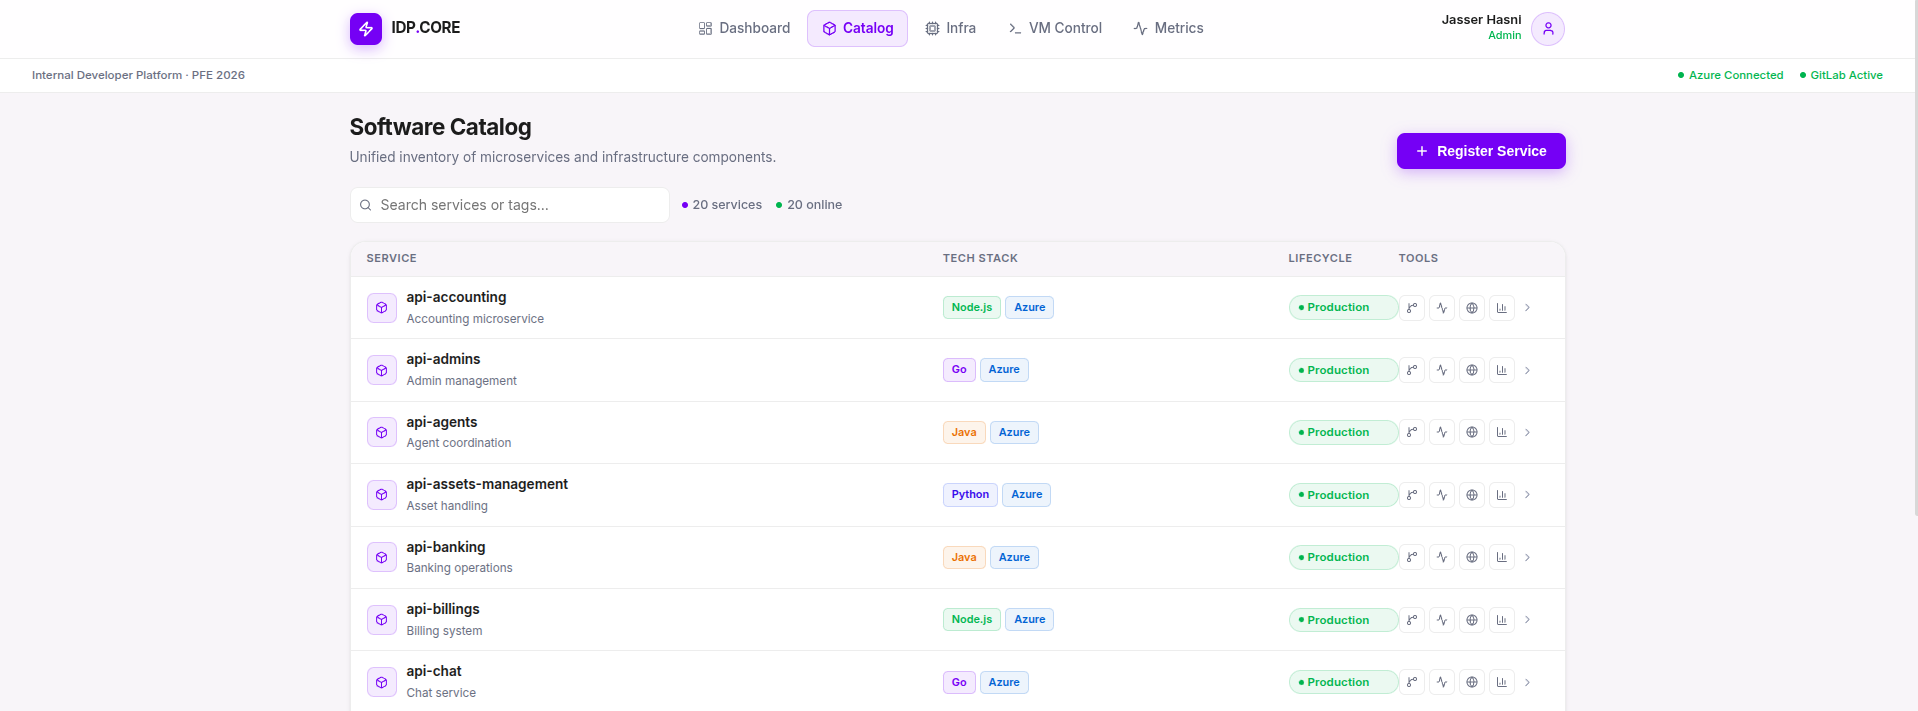
\includegraphics[width=\textwidth]{fig_software_catalog}
  \caption{Software Catalog de l'\ac{IDP} --- vue liste des microservices~\cite{backstage2023catalog}}
  \label{fig:software_catalog}
\end{figure}

\section{Passerelle sécurisée vers Azure --- Proxy Node.js}
\label{sec:proxy_nodejs}

L'\ac{IDP} est intégrée à l'infrastructure cloud Azure par l'intermédiaire d'un \textbf{proxy Node.js} dédié, conçu et développé dans le cadre de ce projet. Ce composant constitue un élément essentiel de l'architecture de la plateforme : il joue le rôle de couche middleware entre Backstage et l'\ac{API} Azure Resource Manager (\textbf{ARM})~\cite{azure2023arm}. Cette architecture met en pratique le principe de \textit{defense in depth} : aucune accréditation Azure n'est exposée à l'interface utilisateur, et toutes les communications entre la plateforme et les services cloud transitent par ce proxy, qui centralise l'authentification, le contrôle d'accès et la journalisation des échanges.

Ce proxy assure l'authentification auprès des services Azure grâce aux \textit{Managed Identities}, la gestion des jetons d'accès à durée de vie courte et l'exécution des requêtes vers les différents services cloud. Il garantit ainsi qu'aucune information sensible --- identifiants, secrets, clés d'accès à l'\ac{API} Azure --- ne soit exposée au niveau de l'interface Backstage. De plus, le proxy implémente une couche de mise en cache des réponses provenant des services Azure, limitant le nombre de requêtes vers l'\ac{API} ARM et assurant des performances satisfaisantes de l'interface utilisateur.

Grâce à l'\ac{API} Azure Resource Manager, le proxy est capable de récupérer l'état des ressources hébergées sur le cloud --- clusters \ac{AKS}, instances de machines virtuelles, groupes de ressources, services associés. Ces informations sont ensuite filtrées, agrégées et présentées sous une forme simplifiée au sein de l'\ac{IDP}, facilitant la prise de décision. La Figure~\ref{fig:proxy_nodejs} illustre l'architecture du proxy en détaillant les couches d'authentification par \textit{Managed Identity}, de mise en cache et de routage vers l'\ac{API} ARM, tandis que la Figure~\ref{fig:proxy_request_example} présente un exemple concret de requête vers l'\ac{API} Azure ARM, illustrant le format des échanges et la structure des réponses renvoyées à l'\ac{IDP}.

%\vspace{0.4cm}
\begin{figure}[htbp]
  \centering
  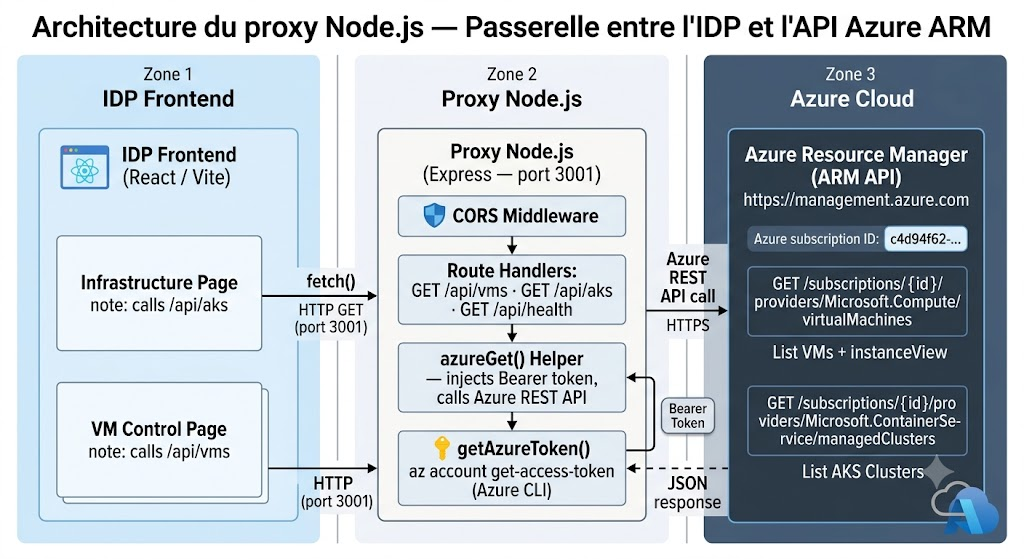
\includegraphics[width=\textwidth]{fig_proxy_nodejs}
  \caption{Architecture du proxy Node.js ~\cite{azure2023arm}}
  \label{fig:proxy_nodejs}
\end{figure}

\begin{figure}[htbp]
  \centering
  %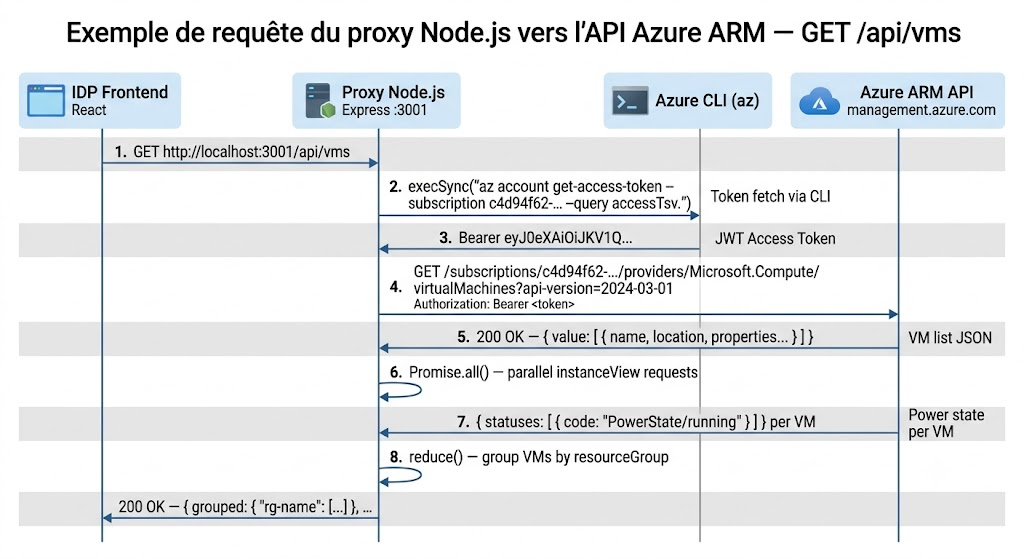
\includegraphics[width=0.99\textwidth,height=11cm]{fig_proxy_request_example}
  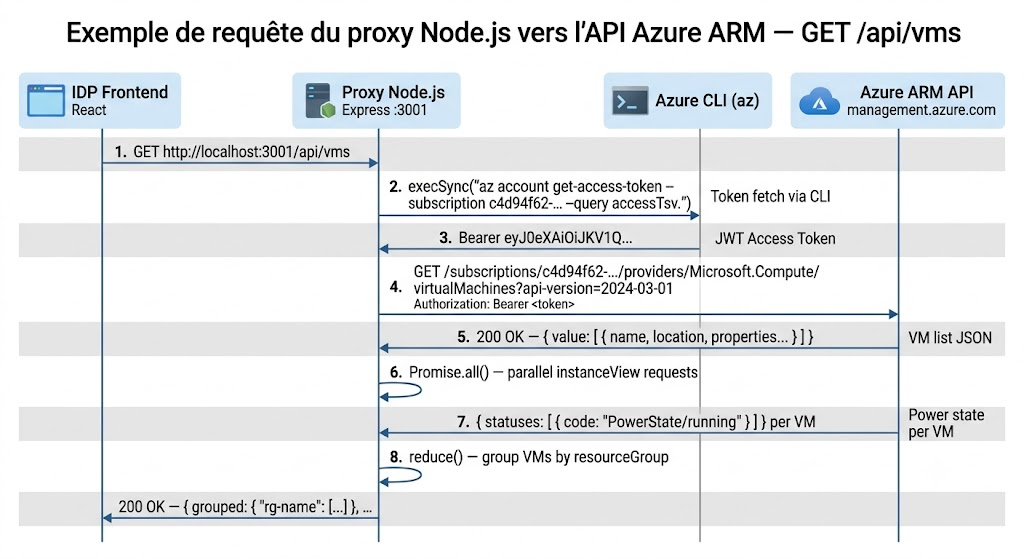
\includegraphics[width=\textwidth]{fig_proxy_request_example}
  \caption{Exemple de requête du proxy Node.js vers l'\ac{API} Azure ARM~\cite{azure2023arm}}
  \label{fig:proxy_request_example}
\end{figure}

\section{Accès aux outils d'observabilité}
\label{sec:acces_outils}

L'\ac{IDP} centralise l'accès à l'ensemble des outils d'observabilité et de gestion opérationnelle utilisés au sein de l'infrastructure, évitant ainsi la navigation entre de multiples interfaces. Dans une architecture microservices mature, la multiplicité des outils de supervision peut elle-même devenir une source de complexité : chaque outil possède sa propre URL, sa propre méthode d'authentification et ses propres conventions de nommage. En l'absence de centralisation, un développeur confronté à un incident doit se souvenir de chaque URL, s'authentifier séparément sur chaque outil et configurer manuellement ses filtres.

La solution adoptée consiste à proposer des liens pré-établis et pré-filtrés pour chaque service vers l'outil de supervision associé. La plateforme intègre ainsi \textit{Grafana} pour la visualisation des métriques et la gestion des indicateurs de performance, \textit{Kibana} pour la lecture et l'analyse des logs applicatifs, et \textit{Jaeger} ainsi que \textit{Tempo} pour le traçage distribué des requêtes au sein de l'architecture microservices. L'un des atouts majeurs de cette architecture est le pré-filtrage des liens selon le service consulté : un développeur qui consulte les informations relatives au microservice \texttt{api-accounting} dans le \textit{Software Catalog} y trouve directement les tableaux de bord Grafana et les index Kibana correspondants à ce service. La Figure~\ref{fig:idp_outils} présente le centre d'accès unifié aux outils d'observabilité depuis l'\ac{IDP}, illustrant comment un développeur accède en un clic aux tableaux de bord Grafana, aux index Kibana et aux traces Jaeger d'un service donné, sans aucune configuration manuelle préalable.

\begin{figure}[htbp]
  \centering
  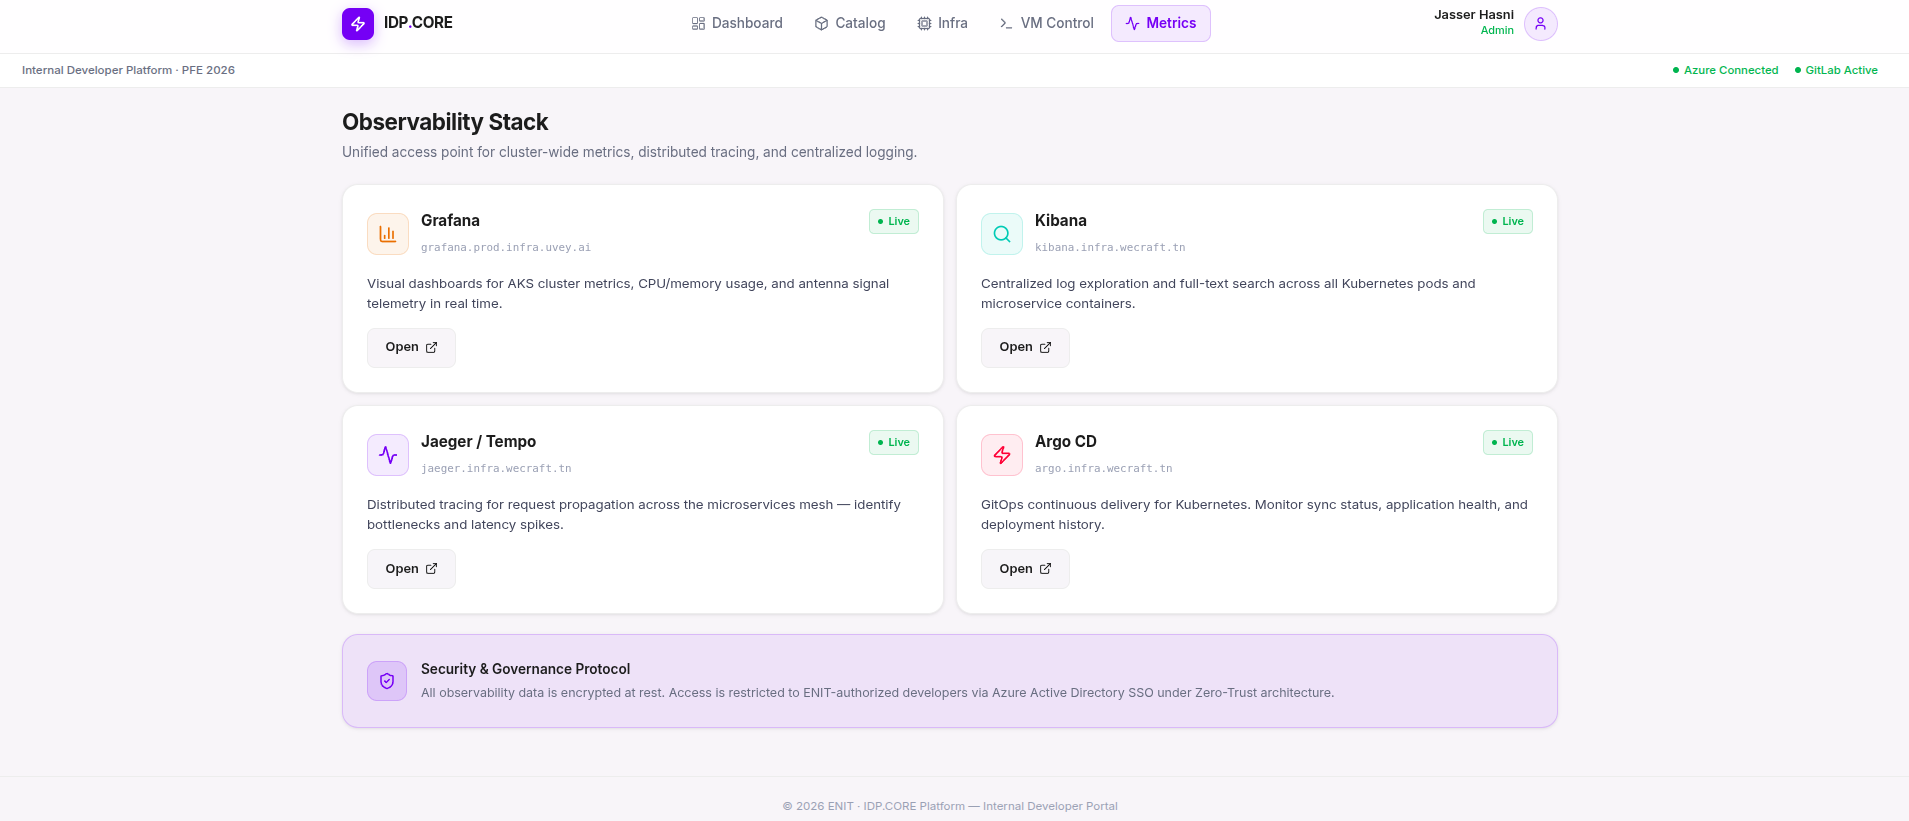
\includegraphics[width=\textwidth]{fig_idp_outils}
  \caption{Centre d'accès unifié aux outils d'observabilité depuis l'\ac{IDP}~\cite{backstage2023docs}}
  \label{fig:idp_outils}
\end{figure}

\section{Gestion des environnements}
\label{sec:gestion_environnements}

La gestion des environnements figure parmi les principaux points de friction identifiés par les équipes de développement dans les organisations adoptant le cloud natif. Le provisionnement d'un environnement de test nécessite généralement la participation de l'équipe infrastructure, la création d'un ticket formel et un délai d'attente pouvant varier de quelques heures à plusieurs jours. Ce processus est incompatible avec les cycles de développement agile, qui exigent un accès immédiat à des environnements de test pour valider des modifications, corriger des anomalies ou réaliser des démonstrations.

\begin{table}[htbp]
  \centering
  \renewcommand{\arraystretch}{1.3}
  \begin{tabularx}{\textwidth}{L{3cm} L{4.5cm} L{4.5cm} C{1.8cm}}
    \toprule
    \rowcolor{uveylight}
    \textbf{Type} & \textbf{Objectif} & \textbf{Caractéristiques} & \textbf{Durée de vie} \\
    \midrule
    Développement   & Tests locaux et intégration continue & Ressources limitées, données de test synthétiques & Permanente \\
    Staging         & Validation préproduction & Miroir de la production, données anonymisées & Permanente \\
    Éphémère (sandbox) & Tests spécifiques à la demande & Créé automatiquement, détruit après usage & 1--72h \\
    \bottomrule
  \end{tabularx}
  \caption{Types d'environnements gérés via l'\ac{IDP}}
  \label{tab:environments}
\end{table}

La Figure~\ref{fig:env_creation} illustre l'interface de création d'un environnement éphémère depuis l'\ac{IDP}, permettant à un développeur de spécifier le type d'environnement souhaité, la durée de vie et les services à déployer, le tout sans aucune intervention de l'équipe infrastructure.

\begin{figure}[htbp]
  \centering
  %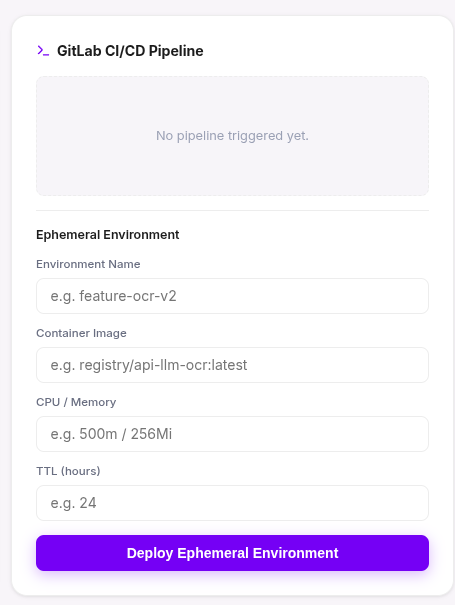
\includegraphics[width=0.95\textwidth,height=12cm]{fig_env_creation}
  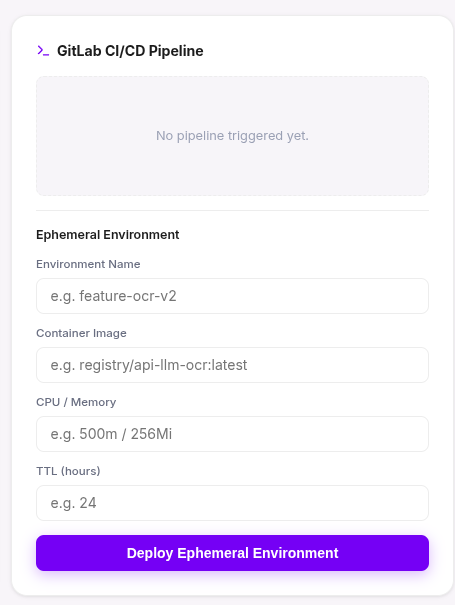
\includegraphics[height=11cm]{fig_env_creation}
  \caption{Interface de création d'un environnement éphémère depuis l'\ac{IDP}~\cite{backstage2023docs}}
  \label{fig:env_creation}
\end{figure}

\section{Réduction de la charge cognitive}
\label{sec:devex}

L'optimisation de l'expérience développeur (\textit{Developer Experience} ou \acf{DX}) représente l'objectif central de tout projet \ac{IDP}. Au-delà des gains de productivité quantifiables, une bonne expérience développeur favorise la satisfaction des équipes, la rétention du personnel et l'attractivité de l'entreprise pour les nouvelles recrues. Selon de récentes recherches~\cite{noda2023devex}, trois éléments constituent les principales sources de friction dans l'expérience développeur : la fragmentation des outils, les longues boucles de feedback et l'absence de documentation à jour. L'\ac{IDP} construite dans le cadre de ce projet est conçue pour adresser spécifiquement ces trois points.

Avant la mise en œuvre de l'\ac{IDP}, les développeurs d'Uvey devaient naviguer entre plusieurs interfaces pour effectuer une opération de déploiement ou de débogage. Ce phénomène de \textit{context switching} créait une charge cognitive supplémentaire qui se répercutait directement sur les performances, allongeant les délais de résolution des incidents. Chaque transition entre interfaces impliquait une nouvelle authentification, une adaptation à un environnement d'interface différent et une re-contextualisation des informations affichées. Le tableau~\ref{tab:context_switching} illustre concrètement les gains apportés par l'\ac{IDP}.

\begin{table}[htbp]
  \centering
  \renewcommand{\arraystretch}{1.3}
  \begin{tabularx}{\textwidth}{L{5cm} C{3cm} C{3cm}}
    \toprule
    \rowcolor{uveylight}
    \textbf{Tâche} & \textbf{Avant IDP} & \textbf{Après IDP} \\
    \midrule
    Déployer un microservice          & 5 outils & 1 interface \\
    Diagnostiquer un incident         & 4 outils & 1 interface \\
    Créer un environnement de test    & Manuel (30 min) & Self-service (5 min) \\
    Accéder à la documentation        & Wiki séparé & Catalogue intégré \\
    Vérifier l'état d'un déploiement  & ArgoCD + portail Azure & 1 interface \\
    Accéder aux métriques d'un service & Grafana (config manuelle) & Lien pré-filtré IDP \\
    Consulter les logs d'un service   & Kibana (config manuelle) & Lien pré-filtré IDP \\
    \bottomrule
  \end{tabularx}
  \caption{Comparaison des flux de travail avant et après l'\ac{IDP}~\cite{noda2023devex}}
  \label{tab:context_switching}
\end{table}

Ce gain quantitatif se traduit également par un bénéfice qualitatif tangible : les développeurs disposent de davantage de temps pour des tâches à haute valeur ajoutée, telles que le développement de nouvelles fonctionnalités ou l'amélioration de la qualité du code, au lieu de consacrer leur attention à la navigation entre les outils. Par ailleurs, la réduction du \ac{MTTR} améliore directement la disponibilité de la plateforme et la satisfaction des utilisateurs finaux d'Uvey.

\section*{Conclusion}
\addcontentsline{toc}{section}{Conclusion}

Ce chapitre a détaillé la mise en œuvre de l'\ac{IDP} basée sur Backstage. Après avoir justifié ce choix technologique par une analyse multicritères comparative, les différentes fonctionnalités du framework ont été présentées : le \textit{Software Catalog} pour la centralisation des services, le proxy Node.js pour une connexion sécurisée entre la plateforme et l'\ac{API} Azure ARM, une interface unifiée d'accès aux outils de monitoring avec des liens filtrés par service, et la gestion entièrement autonome des environnements éphémères en self-service.

Le chapitre suivant traite de la migration vers Azure et de la mise en place de l'infrastructure cloud sous-jacente sur laquelle repose l'\ac{IDP}.

\chapter{Migration vers Azure et Mise en place de l'Infrastructure}
\label{chap:azure}

\section*{Introduction}
\addcontentsline{toc}{section}{Introduction}

\noindent Ce chapitre décrit la migration vers Azure et la création de l'infrastructure cloud sur laquelle repose techniquement l'ensemble de la plateforme. Passer d'une infrastructure existante vers un cloud public de cette envergure constitue un chantier à la fois techniquement complexe et organisationnellement exigeant, qui nécessite des choix d'architecture structurants dès la première phase du projet. Sont passés en revue successivement : l'architecture réseau globale, le déploiement et la segmentation des clusters \ac{AKS}, la gestion des identités selon le principe Zero-Trust, la migration du contrôleur Ingress NGINX vers l'Application Gateway via \ac{AGIC}, la migration de la base de données PostgreSQL depuis \ac{GCP} vers Azure, la gestion automatisée des certificats SSL/TLS, et l'intégration de l'ensemble de ces éléments dans l'\ac{IDP}.

\section{Architecture de l'infrastructure Azure}
\label{sec:architecture_reseau}

\noindent L'infrastructure de référence a été déployée sur Microsoft Azure en suivant une approche d'\acf{IaC} basée sur \tech{Terraform}~\cite{hashicorp2023terraform}. Cette approche garantit la reproductibilité, la traçabilité et l'automatisation de la création et de la gestion de l'ensemble des ressources Azure. La méthode déclarative permet en effet de définir sous forme de code, versionné dans Git, l'ensemble des éléments constitutifs de l'infrastructure : réseaux, clusters, bases de données, politiques de sécurité et identités.

L'architecture, comme le montre la Figure \ref{fig:azure_architecture}, repose sur \ac{AKS}, constitué de plusieurs clusters et services connectés afin d'assurer une bonne répartition des charges, une haute disponibilité des applications et une séparation claire des environnements. Cette architecture multi-clusters apporte une forte isolation entre les workloads : elle évite les problèmes de contention de ressources et permet d'appliquer des politiques de sécurité spécifiques à chaque cluster. Il en résulte notamment une isolation stricte entre les microservices métier et l'infrastructure d'automatisation, telle que les runners de \ac{CI/CD}.

\begin{figure}[H]
  \centering
  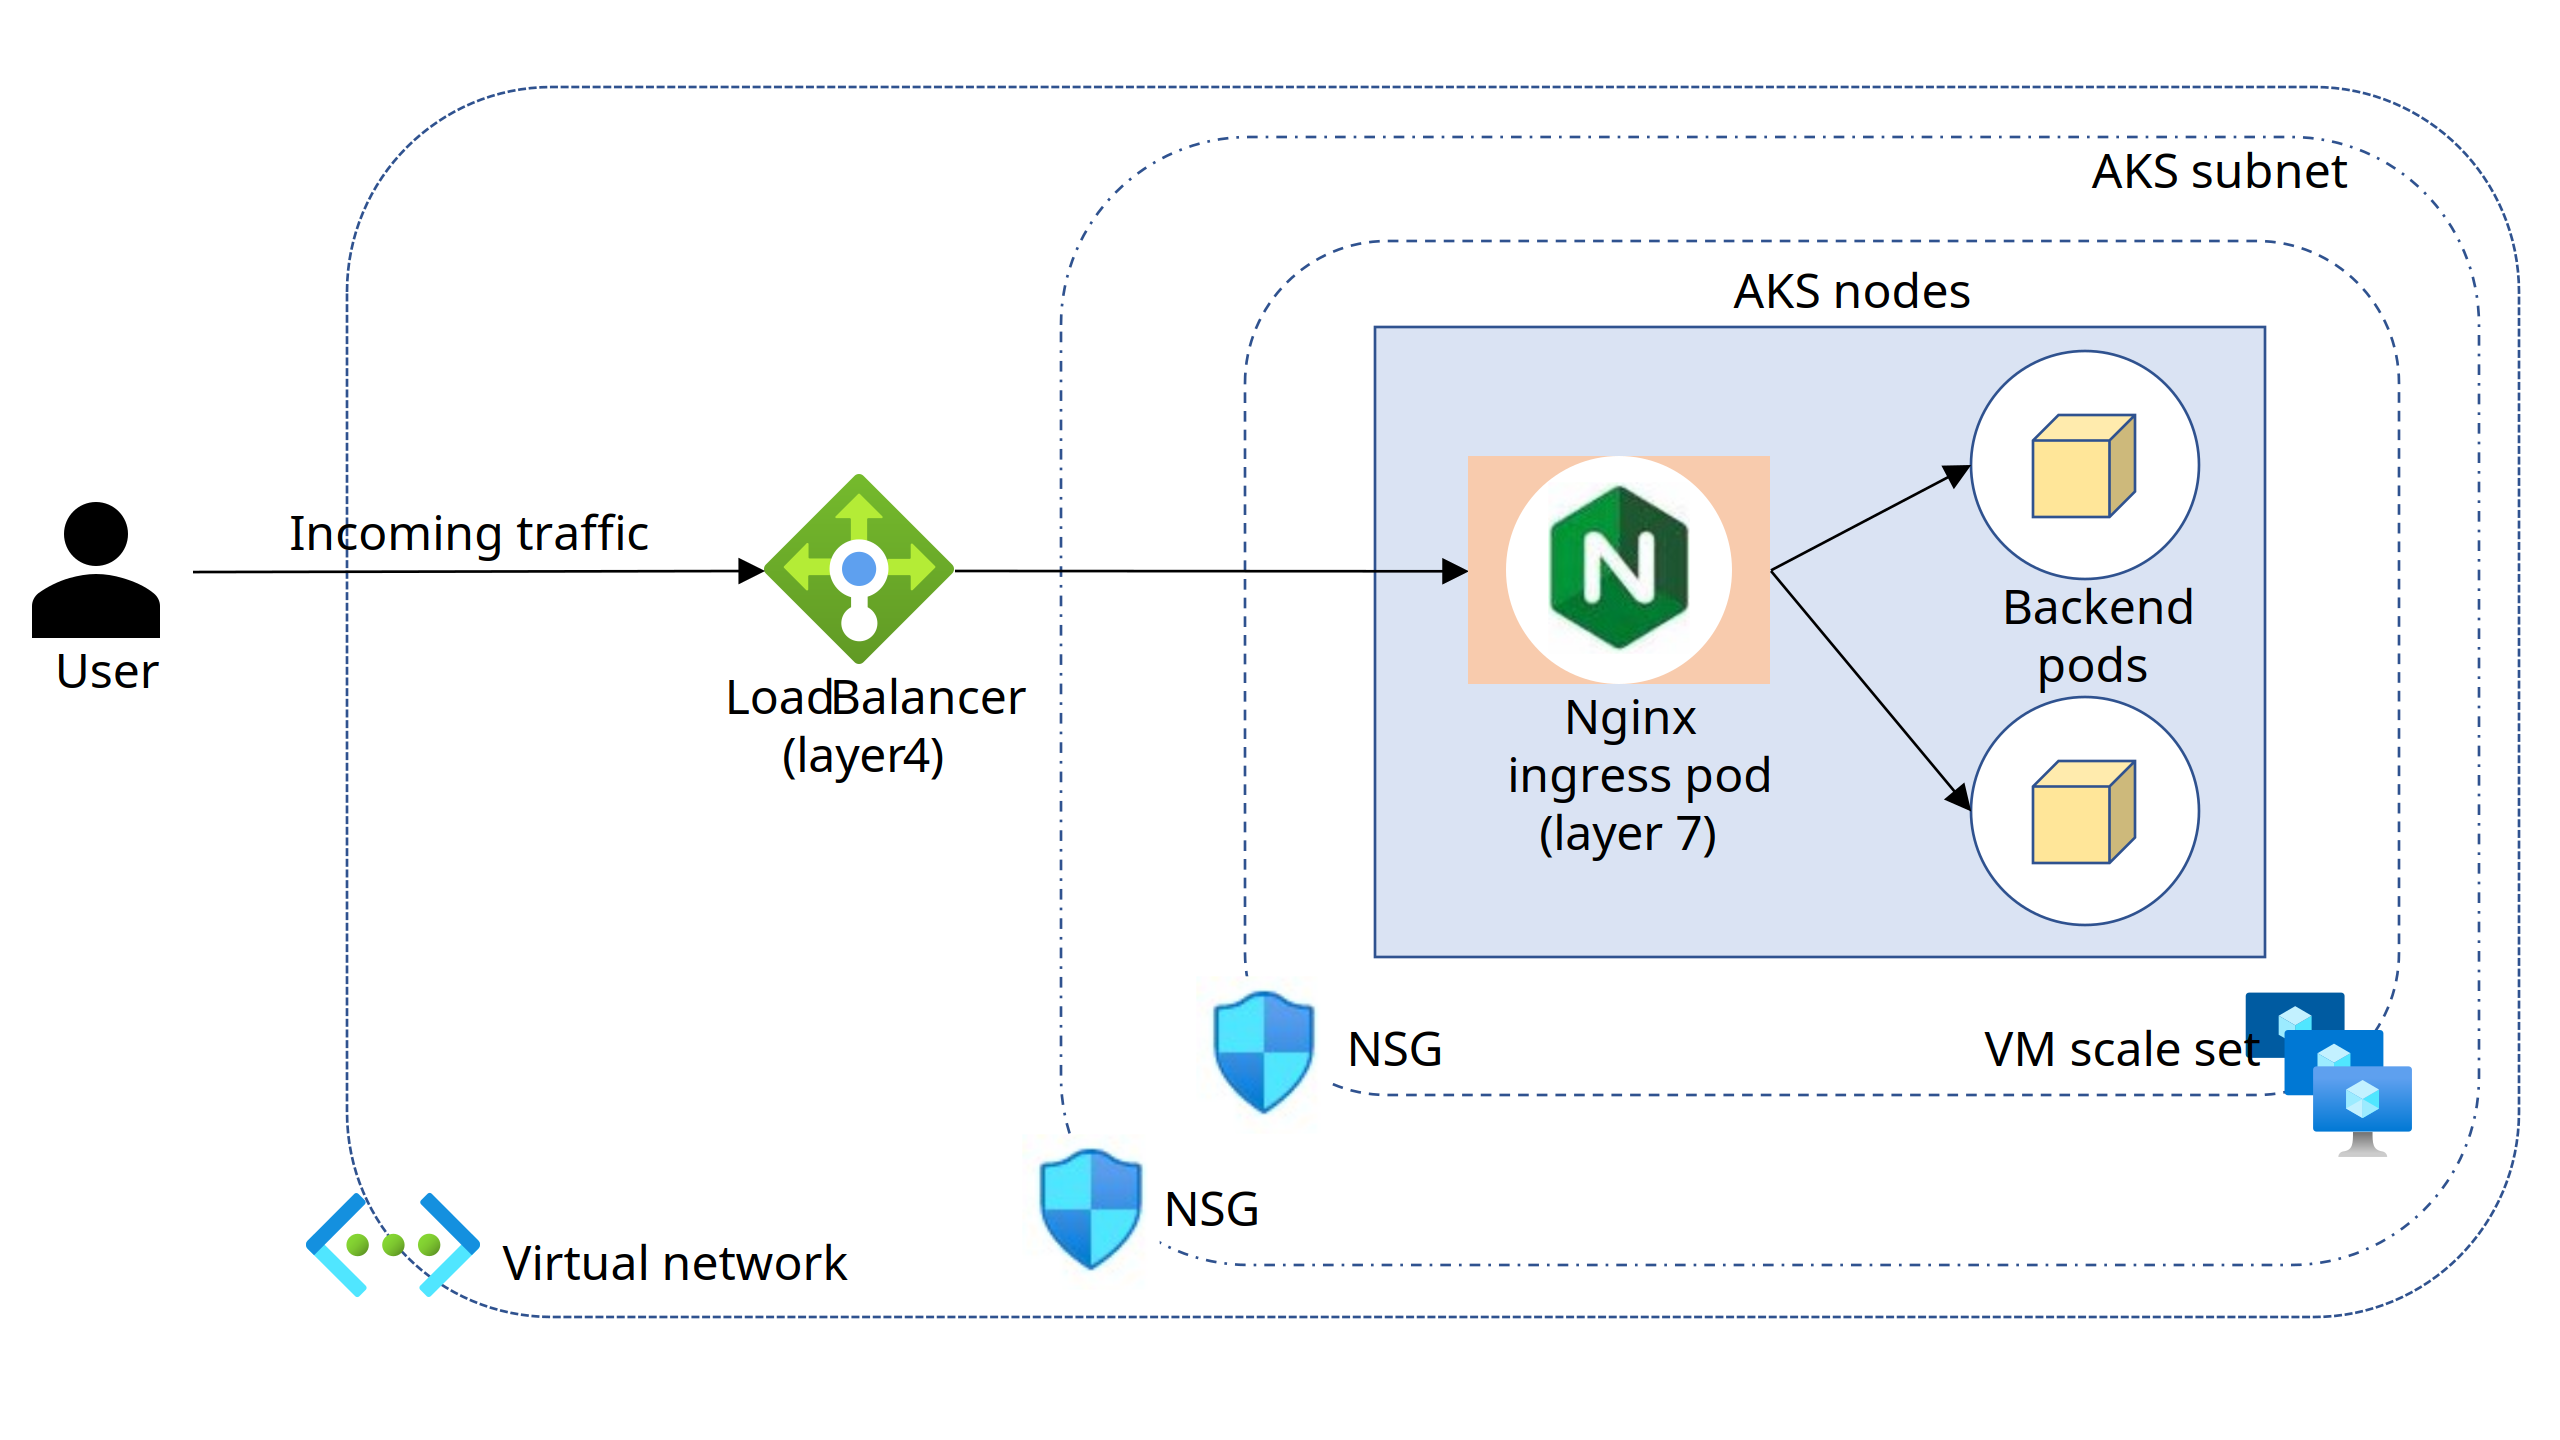
\includegraphics[width=\textwidth]{fig_architecture_azure}
  \caption{Architecture réseau de l'infrastructure Azure AKS~\cite{microsoft2024aksingress}}
  \label{fig:azure_architecture}
\end{figure}

\section{Déploiement et segmentation des clusters AKS}
\label{sec:clusters_aks}

\noindent Cette section présente l'organisation des trois clusters \ac{AKS} déployés, la segmentation réseau adoptée et les choix de plugin réseau qui en découlent.

\subsection{Organisation des clusters}

Trois clusters \ac{AKS} distincts ont été mis en place afin de distinguer avec précision les environnements et les rôles. En répartissant les charges de travail sur trois clusters dédiés, il est possible de réduire drastiquement le périmètre d'impact (\textit{blast radius}) en cas de dysfonctionnement ou d'opération non souhaitée. Ce découpage a également des conséquences sur la gouvernance : chaque cluster dispose de son propre cadre \ac{RBAC}, de son propre quota de ressources et de sa propre politique réseau, comme le résume le tableau~\ref{tab:clusters_aks}.

\begin{table}[H]
  \centering
 
  \renewcommand{\arraystretch}{1.4}
  \begin{tabularx}{\textwidth}{L{2.8cm} L{5.5cm} L{5.5cm}}
    \toprule
    \rowcolor{uveylight}
    \textbf{Cluster} & \textbf{Rôle} & \textbf{Workloads principaux} \\
    \midrule
    \texttt{uvey} (applicatif) & Hébergement des microservices métier & \texttt{api-accounting}, \texttt{api-llm-ocr}, \texttt{api-gateway}, services Node.js/Go/Java/Python/C\# \\
    \midrule
    Automation & Outils DevOps transverses & Stack ELK, Prometheus, Grafana, gestionnaire de secrets \\
    \midrule
    GitLab CI/CD   & Exécution des pipelines \ac{CI/CD} & Runners GitLab haute capacité CPU pour builds parallèles \\
    \bottomrule
  \end{tabularx}
  \caption{Description des trois clusters AKS déployés~\cite{azure2023aks}}
   \label{tab:clusters_aks}
\end{table}

\subsection{Architecture réseau et choix du plugin CNI}

L'ensemble des ressources réside dans un seul réseau virtuel Azure (\ac{VNet})~\cite{azure2023vnet}, subdivisé en sous-réseaux aux périmètres distincts : Application Gateway (seul sous-réseau ouvert vers Internet), AKS (nœuds de calcul avec Azure \ac{CNI}), PostgreSQL (entièrement privé avec \textit{Private DNS Zone}), et sous-réseaux temporaires pour le bastion de migration. Le plugin réseau \textit{Azure CNI} a été préféré à Kubenet de manière délibérée : chaque pod obtient une adresse IP directement issue du sous-réseau \ac{VNet}, ce qui permet une interaction native avec l'environnement Azure, simplifie le débogage réseau et élimine la couche de traduction d'adresses NAT qu'introduit Kubenet, laquelle peut compliquer le contrôle des politiques réseau en production. Les \textit{Network Policies} Kubernetes sont activées sur l'ensemble des clusters afin d'implémenter le modèle de communication inter-pods selon le principe du moindre privilège. Le tableau~\ref{tab:cni_comparaison} présente la comparaison des deux options. La Figure~\ref{fig:vnet} représente la topologie du \ac{VNet} et la répartition des sous-réseaux, faisant apparaître l'isolation entre le sous-réseau exposé de l'Application Gateway, les sous-réseaux de calcul AKS et le sous-réseau entièrement privé de la base de données PostgreSQL.

\begin{table}[H]
  \centering
  \renewcommand{\arraystretch}{1.3}
  \begin{tabularx}{\textwidth}{L{4cm} L{5cm} L{5cm}}
    \toprule
    \rowcolor{uveylight}
    \textbf{Critère} & \textbf{Azure CNI} & \textbf{Kubenet} \\
    \midrule
    Adressage des pods     & IP du sous-réseau VNet (routable) & IP privée traduite par NAT \\
    Intégration services Azure & Native (NSG, Private Link) & Limitée (NAT intermédiaire) \\
    Débogage réseau        & Simplifié (IP directement visible) & Complexifié (masquage NAT) \\
    Network Policies       & Supportées nativement & Supportées (avec plugin Calico) \\
    Consommation d'IP      & Plus élevée (1 IP/pod) & Réduite (IP partagée par nœud) \\
    Cas d'usage optimal    & Production, intégration VNet poussée & Clusters à faible densité IP \\
    \textbf{Choix}         & \textbf{Retenu} & Non retenu \\
    \bottomrule
  \end{tabularx}
  \caption{Comparaison des plugins réseau AKS --- Azure CNI vs Kubenet}
  \label{tab:cni_comparaison}
\end{table}

\begin{figure}[H]
  \centering
  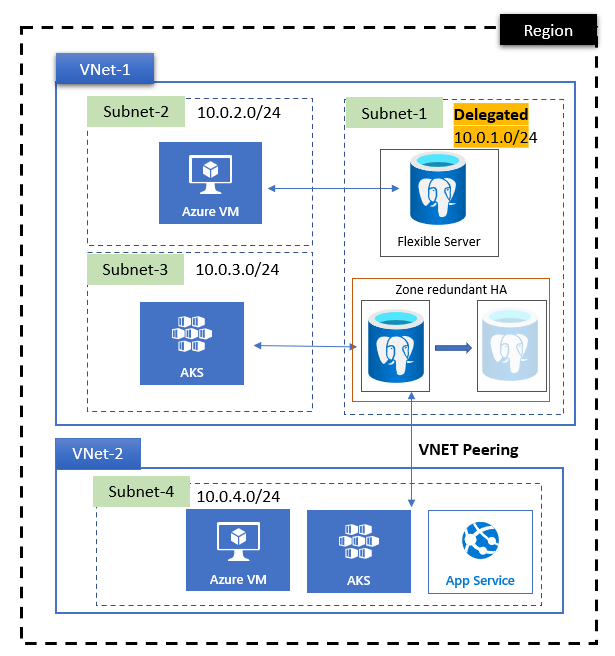
\includegraphics[width=0.75\textwidth]{fig_vnet_subnets}
  \caption{Architecture du \ac{VNet} Azure et intégration réseau~\cite{microsoft2024pgvnet}}
  \label{fig:vnet}
\end{figure}

\section{Authentification Zero-Trust avec Managed Identities}
\label{sec:zerotrust}

\noindent La gestion de l'authentification et de l'identité est assurée via Azure Active Directory avec une \textit{Managed Identity} assignée à chaque cluster, selon le principe du \textbf{Zero-Trust}~\cite{nist2020zerotrust} : aucun secret d'accès statique n'est utilisé pour les communications entre services Azure. Cette décision architecturale supprime une catégorie entière de vulnérabilités liées à la gestion des secrets : rotation oubliée, diffusion accidentelle dans un dépôt Git, ou exposition dans les variables d'environnement d'un conteneur.

Concrètement, une \textit{Managed Identity} est une identité gérée par Azure Active Directory avec un cycle de vie complet --- création, rotation automatique du jeton, révocation --- sans que la gestion des secrets entre jamais dans le périmètre des opérations de l'équipe. Chaque cluster \ac{AKS} bénéficie d'une identité propre à laquelle sont attribuées des permissions \ac{RBAC} minimales, limitées aux ressources Azure strictement requises : accès en lecture au registre de conteneurs, accès en écriture aux \textit{Managed Disks} pour les volumes persistants, et accès au \textit{Key Vault} pour les certificats. La comparaison avec l'approche classique par secrets statiques est présentée dans le tableau~\ref{tab:managed_identities}.

\begin{table}[H]
  \centering
  \renewcommand{\arraystretch}{1.3}
  \begin{tabularx}{\textwidth}{L{4.5cm} L{4.5cm} L{4.5cm}}
    \toprule
    \rowcolor{uveylight}
    \textbf{Critère} & \textbf{Managed Identities} & \textbf{Secrets statiques (Service Principal)} \\
    \midrule
    Gestion du cycle de vie  & Automatique (Azure AD) & Manuelle (rotation périodique) \\
    Risque de fuite          & Nul (aucun secret manipulé) & Élevé (variables d'env., Git) \\
    Rotation des credentials & Automatique et transparente & Manuelle, source d'oublis \\
    Auditabilité             & Native (Azure AD logs) & Partielle \\
    Intégration AKS          & Native (add-on AAD Pod Identity) & Configuration manuelle \\
    Conformité Zero-Trust    & Totale & Partielle \\
    \textbf{Choix}           & \textbf{Retenu} & Non retenu \\
    \bottomrule
  \end{tabularx}
  \caption{Comparaison Managed Identities vs secrets statiques}
  \label{tab:managed_identities}
\end{table}

\section{Choix des types de machines virtuelles}
\label{sec:vm_types}

Les node pools sont configurés avec des machines virtuelles de la série E, des instances optimisées pour la mémoire et offrant environ 8 Gio de mémoire par vCPU. Ce choix est motivé par les exigences spécifiques des charges de travail déployées, notamment les composants d'observabilité à forte consommation mémoire, tels que la pile ELK et les traitements \ac{OCR}.

ElasticSearch nécessite une quantité importante de mémoire, car les segments d'indexation et le cache des requêtes sont stockés dans le tas (\textit{heap}) de la JVM. Des nœuds sous-dimensionnés se traduisent par des latences d'indexation dues à des cycles de collecte des objets trop fréquents, voire des erreurs \textit{OutOfMemory} lors de fortes sollicitations. Les modèles d'intelligence artificielle utilisés dans le module \ac{OCR} d'Uvey présentent également des besoins mémoire importants. Par ailleurs, le choix de la génération v5 de la série E est plus avantageux sur le plan des coûts, grâce aux processeurs Intel Ice Lake de dernière génération et à une bande passante mémoire plus élevée, comme le détaille le tableau~\ref{tab:vm_types}.

\begin{table}[htbp]
  \centering
  \renewcommand{\arraystretch}{1.3}
  \begin{tabularx}{\textwidth}{L{3cm} C{3cm} C{2.5cm} C{2.5cm} L{2.5cm}}
    \toprule
    \rowcolor{uveylight}
    \textbf{Cluster} & \textbf{SKU VM} & \textbf{vCPU} & \textbf{Mémoire (Gio)} & \textbf{Justification} \\
    \midrule
    Applicatif     & \texttt{Standard\_E4s\_v5}  & 4   & 32  & Charges de travail à forte consommation mémoire \\
    Automation & \texttt{Standard\_E8s\_v5}  & 8   & 64  & Plateforme d'observabilité (ELK, Prometheus, Loki et Tempo) \\
    GitLab CI/CD   & \texttt{Standard\_E16s\_v5} & 16  & 128 & Pics de charge processeur lors des compilations parallèles \\
    \bottomrule
  \end{tabularx}
  \caption{Récapitulatif des types de machines virtuelles utilisés par cluster~\cite{azure2023vm}}
   \label{tab:vm_types}
\end{table}

\section{Gestion de l'infrastructure avec Terraform}
\label{sec:terraform_pipeline}

\noindent Cette section décrit la stratégie de gestion de l'infrastructure via Terraform, en abordant successivement le pipeline d'automatisation nocturne et la structure modulaire du dépôt.

\subsection{Pipeline d'automatisation nocturne}

Un pipeline GitLab \ac{CI/CD} est mis en place pour automatiser le cycle de vie de l'infrastructure. Ce processus exécute chaque jour une séquence composée d'un \texttt{terraform plan} suivi d'un \texttt{terraform apply}, déclenchée automatiquement à \textbf{22h00}.

Plusieurs garanties ont été prévues pour encadrer ce processus et limiter les risques inhérents à un \texttt{terraform apply} entièrement automatisé dans un environnement de production. Tout d'abord, le pipeline réalise systématiquement un \texttt{terraform plan}, rendu visible via un mécanisme d'approbation dans GitLab (\textit{protected environment with manual gate}) : un membre de l'équipe infrastructure approuve chaque soir le plan calculé au cours des vingt-quatre heures écoulées avant que l'\texttt{apply} ne soit déclenché. Ensuite, les ressources hautement sensibles --- destruction de clusters, modifications de sous-réseaux, modifications de base de données --- sont protégées via le paramètre \texttt{lifecycle \{ prevent\_destroy = true \}} du module Terraform, ce qui entraîne le rejet du plan si une telle action est déclenchée par inadvertance. L'état Terraform (\textit{Terraform State}) est versionné via Azure Blob Storage avec la protection contre les exécutions simultanées activée. Enfin, en cas d'anomalie détectée lors du plan --- destruction de ressource non prévue ou modification hors périmètre --- l'équipe est alertée via le canal de communication dédié et le pipeline est bloqué. La Figure~\ref{fig:terraform_pipeline} présente un extrait du pipeline nocturne au moment de l'étape \texttt{terraform apply}, illustrant la séquence d'exécution des étapes ainsi que le mécanisme d'approbation manuelle avant déploiement.

\begin{figure}[H]
  \centering
  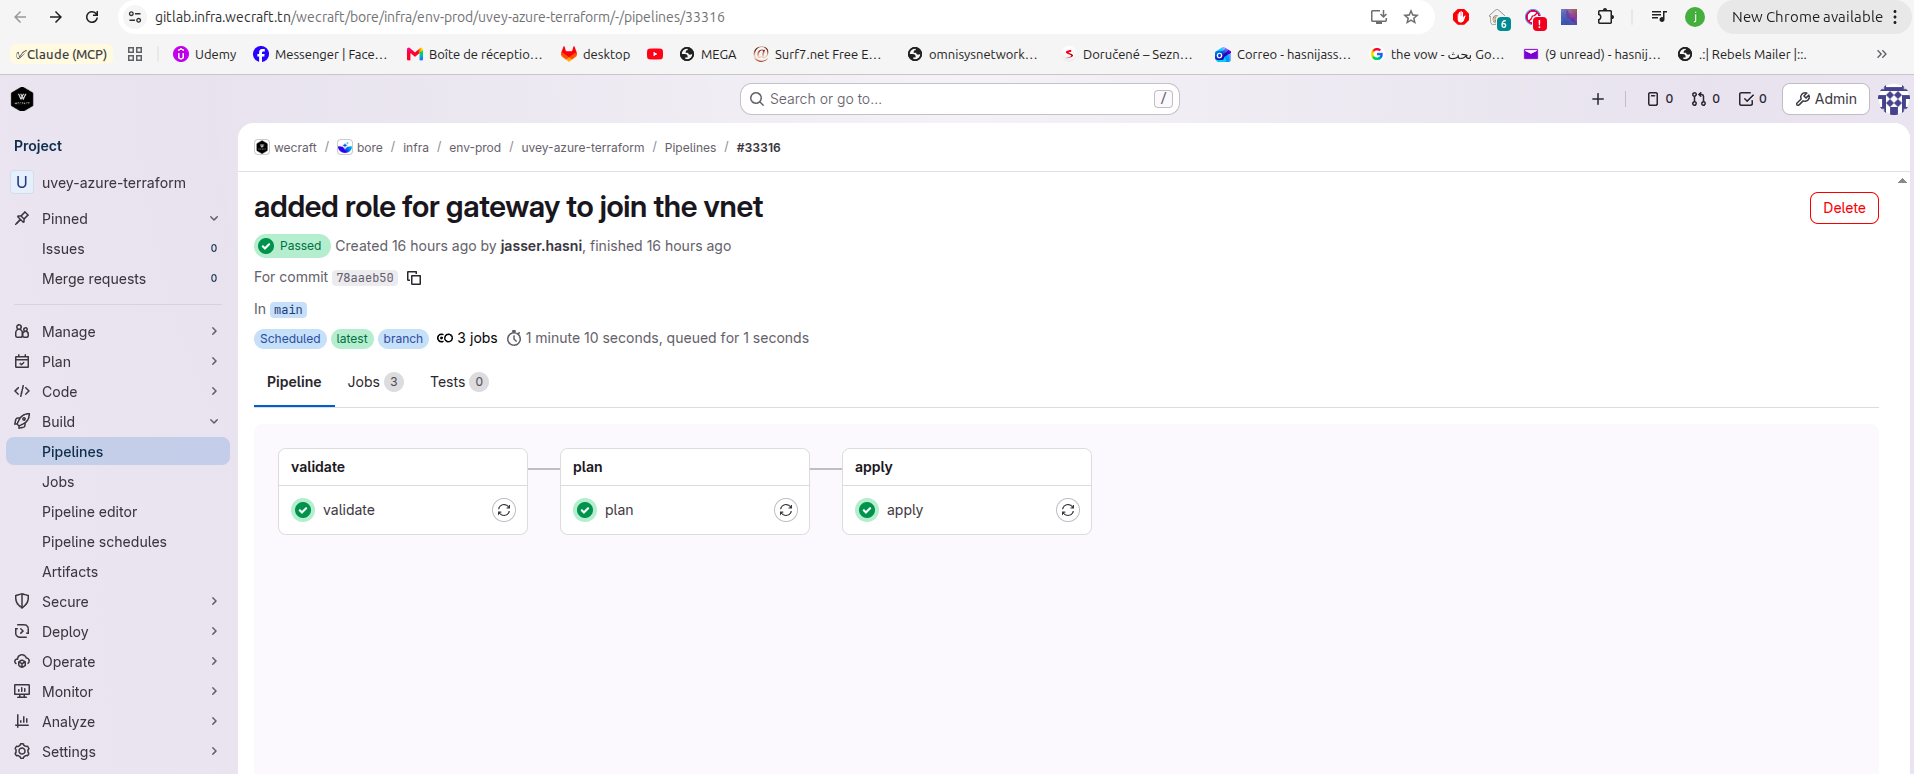
\includegraphics[width=0.90\textwidth]{fig_terraform_pipeline}
  \caption{Étape d'application Terraform --- extrait du pipeline \ac{CI/CD} nocturne~\cite{hashicorp2023terraform}}
  \label{fig:terraform_pipeline}
\end{figure}

\subsection{Structure modulaire du dépôt Terraform}

L'ensemble de l'infrastructure Azure est modélisé selon le principe \ac{IaC} via Terraform, dans lequel toute ressource est définie de manière déclarative, automatisée et versionnée. Afin d'assurer une maintenabilité et une évolution optimales, les ressources cloud sont structurées en modules réutilisables, stockés dans un dépôt Git unique. Cette organisation favorise la standardisation, la réduction de la redondance de code et la cohérence architecturale entre les différents environnements de développement, de tests et de production.

Chaque module Terraform regroupe un ensemble cohérent de ressources réalisant une tâche spécifique. Il existe ainsi des modules dédiés à la gestion des clusters \ac{AKS}, du réseau virtuel Azure, des bases de données PostgreSQL, de l'Application Gateway, du stockage, etc. Chaque module définit une interface claire via des variables d'entrée pour sa configuration et des variables de sortie (\textit{outputs}) facilitant l'intégration avec les autres composants de l'infrastructure. Cette approche rend les composants réutilisables, maintenables et testables lors des phases d'intégration continue.

L'état de l'infrastructure constitue un élément fondamental de cette architecture. Pour garantir l'existence d'une source unique de vérité sur l'état des infrastructures déployées, les états Terraform sont stockés de manière centralisée sur Azure Blob Storage, bénéficiant ainsi de la haute disponibilité et de la durabilité offertes par ce service. La Figure~\ref{fig:terraform_structure} illustre l'organisation du dépôt Terraform en modules réutilisables, faisant apparaître la séparation entre les modules de réseau, de clusters AKS, de base de données et de sécurité, ainsi que le mécanisme de stockage centralisé de l'état sur Azure Blob Storage.

\begin{figure}[H]
  \centering
  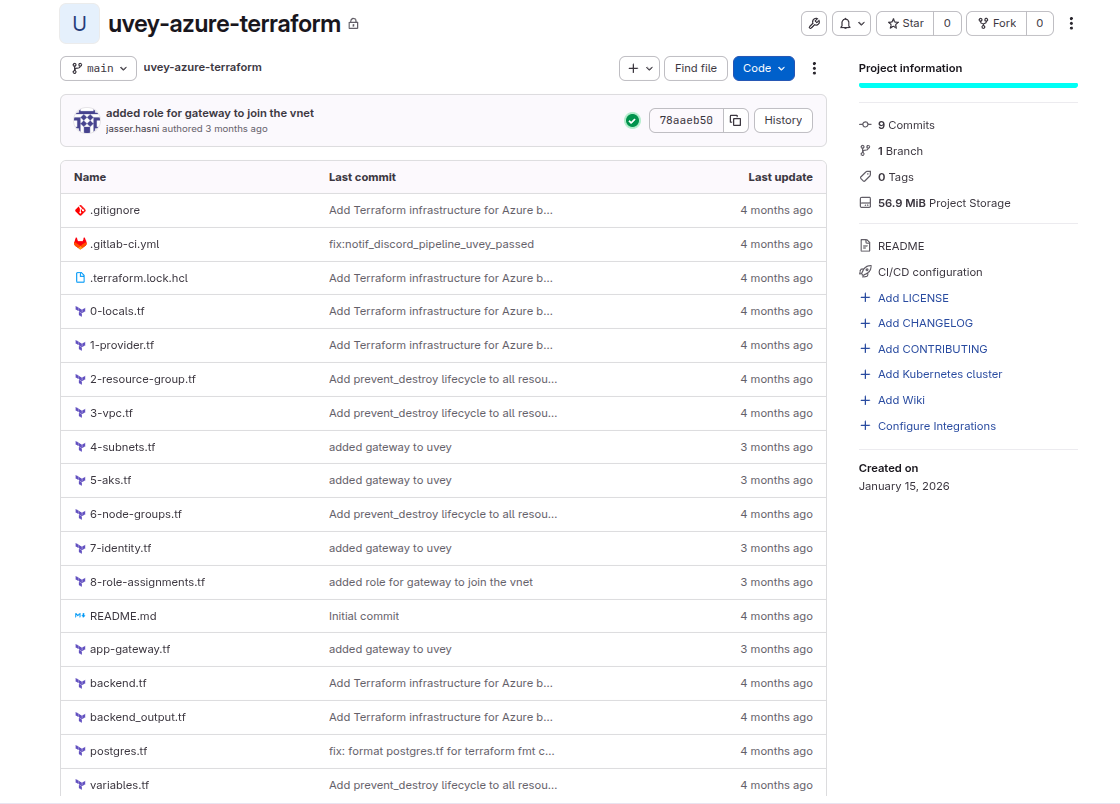
\includegraphics[width=0.88\textwidth]{fig_terraform_structure}
  \caption{Structure du dépôt Terraform pour l'infrastructure Azure~\cite{hashicorp2023terraform}}
  \label{fig:terraform_structure}
\end{figure}

\section{Remplacement de l'Ingress NGINX par l'Application Gateway avec AGIC}
\label{sec:agic}

\noindent Le contrôleur \textbf{Ingress NGINX}~\cite{nginx2023ingress} assurait initialement le routage des services HTTP et HTTPS dans le cluster \ac{AKS}. Cependant, ce composant présente plusieurs inconvénients structuraux dans un contexte de production à grande échelle : consommation de ressources CPU et mémoire sur les nœuds applicatifs, configuration manuelle de la haute disponibilité, et risques de compatibilité avec Kubernetes lors des mises à jour. Par ailleurs, la terminaison TLS sur les pods NGINX consomme des ressources de calcul qui pourraient être allouées aux microservices métiers.

La solution adoptée est fondée sur l'Azure Application Gateway~\cite{azure2023appgw}, associé à l'extension \acf{AGIC}~\cite{azure2023agic}. Cette approche transfère la logique de routage en dehors du cluster tout en conservant une intégration native avec Kubernetes, et incorpore nativement la protection \ac{WAF} avec le ruleset OWASP 3.x. L'\ac{AGIC} surveille en permanence les objets Ingress Kubernetes et convertit automatiquement ces règles en configuration Application Gateway via l'\ac{API} ARM, sans nécessiter d'ajustement manuel de la configuration du load balancer. La configuration \texttt{Standard\_v2} d'Azure Application Gateway garantit une disponibilité contractuelle de 99,95\% fournie par Microsoft. Le tableau~\ref{tab:nginx_vs_agic} compare les deux approches, et la Figure~\ref{fig:agic_architecture} représente la migration depuis Ingress NGINX vers l'Application Gateway, mettant en évidence le déplacement de la terminaison TLS et du routage hors du cluster ainsi que l'intégration native d'\ac{AGIC} avec les objets Ingress Kubernetes.

\begin{figure}[H]
  \centering
  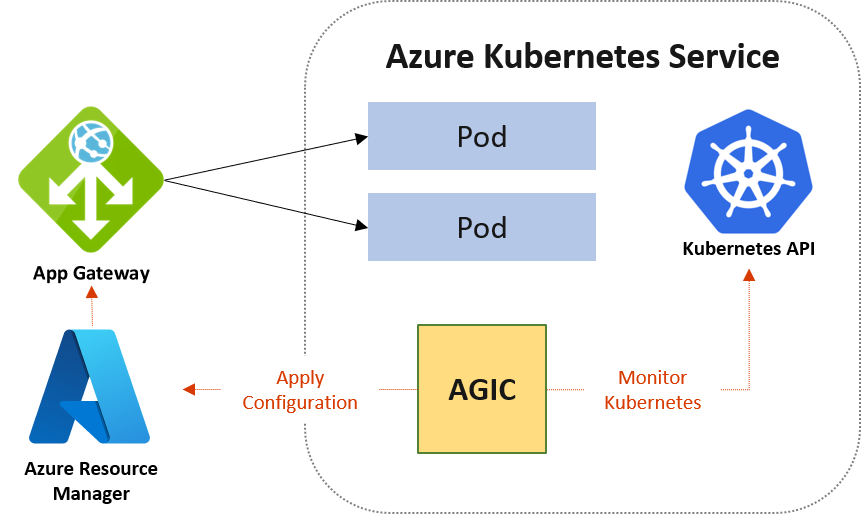
\includegraphics[width=0.8\textwidth]{fig_agic_vs_nginx}
  \caption{Migration de l'Ingress NGINX vers l'Application Gateway avec AGIC~\cite{azure2023agic}}
  \label{fig:agic_architecture}
\end{figure}

\begin{table}[H]
  \centering
  \renewcommand{\arraystretch}{1.3}
  \begin{tabularx}{\textwidth}{L{4cm} L{5cm} L{5cm}}
    \toprule
    \rowcolor{uveylight}
    \textbf{Critère} & \textbf{Ingress NGINX} & \textbf{Application Gateway + AGIC} \\
    \midrule
    Terminaison TLS     & Dans le cluster (pod NGINX) & Hors cluster (service managé Azure) \\
    Consommation cluster & CPU et mémoire des nœuds & Aucune charge sur le cluster \\
    Haute disponibilité  & Configuration manuelle (HPA / replicas) & Nativement intégrée (\texttt{Standard\_v2}) \\
    Protection WAF       & Optionnelle (ModSecurity) & Intégrée (OWASP 3.x) \\
    Gestion des certificats & cert-manager ou secrets Kubernetes & Intégration Azure Key Vault \\
    SLA Azure            & Non applicable & 99,95\% (\texttt{Standard\_v2}) \\
    \bottomrule
  \end{tabularx}
  \caption{Comparaison entre Ingress NGINX et Application Gateway avec AGIC~\cite{azure2023agic}}
  \label{tab:nginx_vs_agic}
\end{table}

La Figure~\ref{fig:agic_terraform} présente l'activation d'\ac{AGIC} en tant qu'add-on managé sur le cluster AKS via Terraform, illustrant comment l'add-on est déclaré directement dans la ressource \texttt{azurerm\_kubernetes\_cluster} et lié à l'instance d'Application Gateway provisionnée dans le même module.

\begin{figure}[H]
  \centering
  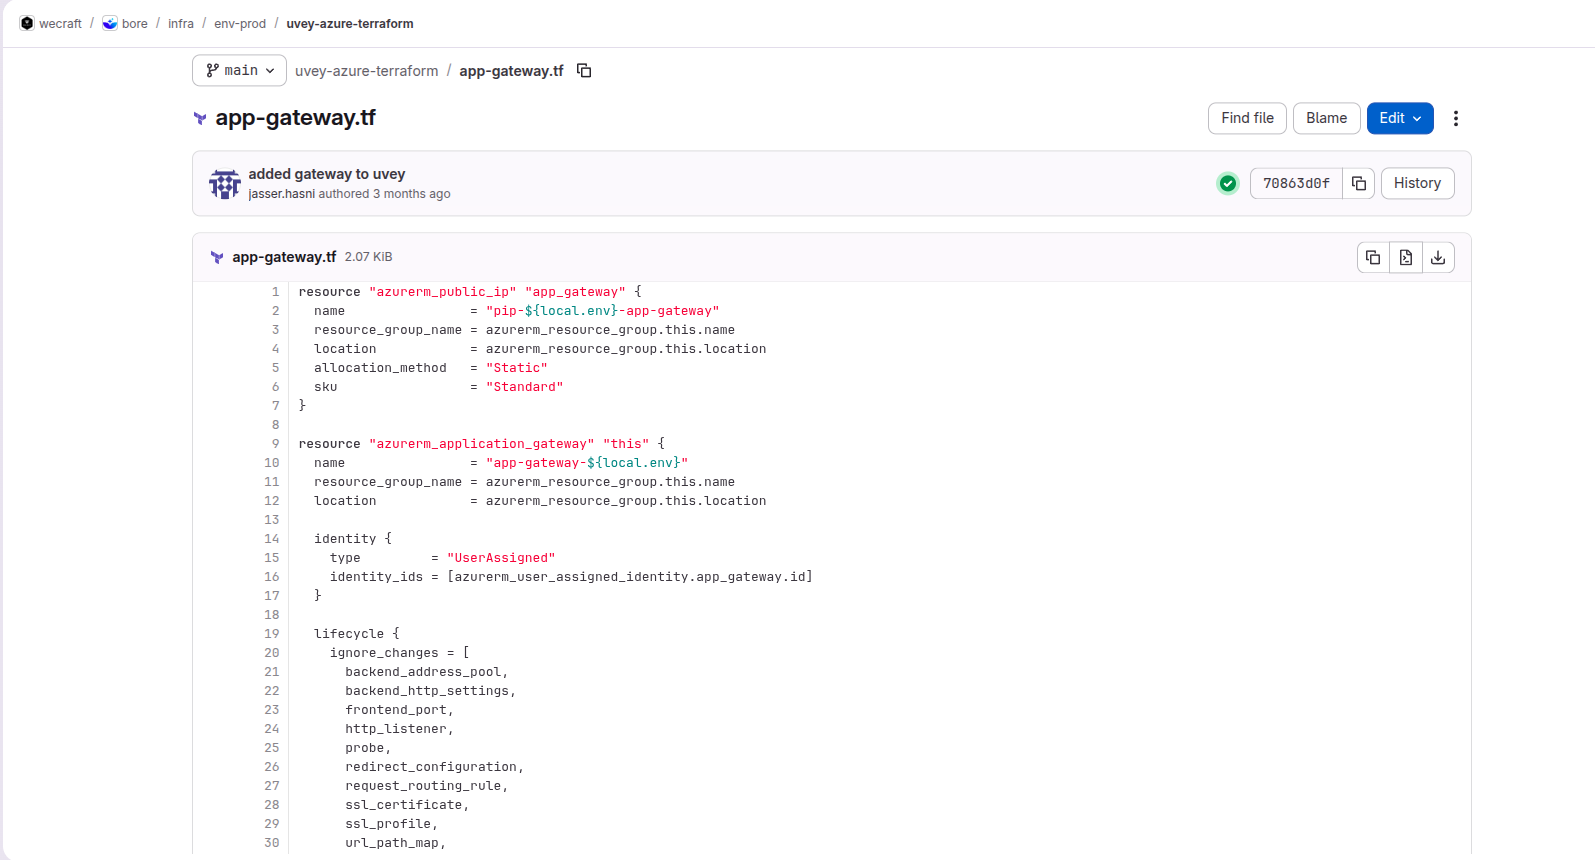
\includegraphics[width=0.88\textwidth]{fig_agic_terraform}
  \caption{Activation d'\ac{AGIC} comme add-on managé sur le cluster AKS~\cite{azure2023agic}}
  \label{fig:agic_terraform}
\end{figure}


\section{Gestion des certificats SSL/TLS avec cert-manager}
\label{sec:certmanager}

\noindent L'automatisation du cycle de vie des certificats SSL/TLS est assurée par \tech{cert-manager}~\cite{certmanager2023docs}, déployé sur l'ensemble des clusters \ac{AKS}. Avant la mise en place de cet outil, les certificats étaient gérés manuellement, ce qui entraînait des erreurs fréquentes et des risques de non-renouvellement en temps voulu, pouvant mener à des interruptions de service visibles par les clients. L'utilisation de cert-manager permet la génération des certificats via le fournisseur \textit{Let's Encrypt}~\cite{letsencrypt2023}, leur renouvellement automatique vingt-et-un jours avant expiration, et leur stockage sécurisé dans les secrets Kubernetes.

Le protocole de validation DNS-01 a été retenu en lieu et place d'HTTP-01 pour les raisons détaillées dans le tableau~\ref{tab:certmanager_comparaison} : il prend en charge les domaines internes, les certificats wildcard (\texttt{*.uvey.tn}) et ne nécessite pas l'exposition du port 80 sur Internet. La Figure~\ref{fig:certmanager} illustre le flux complet de gestion des certificats, depuis la création d'un objet \texttt{Certificate} Kubernetes jusqu'à la validation DNS-01 par Let's Encrypt et le stockage automatique du certificat signé dans un secret Kubernetes, le tout sans intervention manuelle.

\begin{table}[H]
  \centering
  \renewcommand{\arraystretch}{1.3}
  \begin{tabularx}{\textwidth}{L{4.5cm} L{4.5cm} L{4.5cm}}
    \toprule
    \rowcolor{uveylight}
    \textbf{Critère} & \textbf{DNS-01} & \textbf{HTTP-01} \\
    \midrule
    Domaines internes      & Supportés & Non supportés \\
    Certificats wildcard   & Supportés (\texttt{*.uvey.tn}) & Non supportés \\
    Exposition Internet    & Non requise & Requise (port 80 ouvert) \\
    Validation via         & Enregistrement DNS TXT & Fichier servi en HTTP \\
    Automatisation         & Via API DNS Azure & Via Ingress HTTP \\
    Cas d'usage optimal    & Domaines privés, wildcard & Services publics simples \\
    \textbf{Choix}         & \textbf{Retenu} & Non retenu \\
    \bottomrule
  \end{tabularx}
  \caption{Comparaison des protocoles de validation cert-manager}
  \label{tab:certmanager_comparaison}
\end{table}

\noindent Cert-manager s'intègre nativement avec les objets Ingress : il suffit d'annoter un Ingress avec le nom de l'émetteur (\texttt{ClusterIssuer}) pour que cert-manager prenne en charge automatiquement l'intégralité du cycle d'émission et de renouvellement du certificat associé.

\begin{figure}[H]
  \centering
  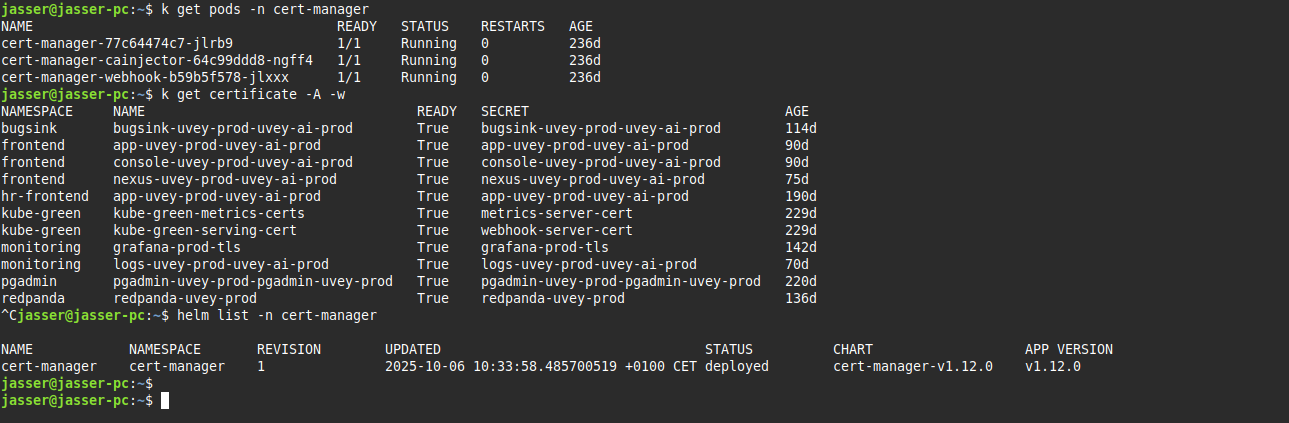
\includegraphics[width=0.88\textwidth]{fig_certmanager}
  \caption{Flux de gestion des certificats SSL/TLS avec Let's Encrypt~\cite{certmanager2023docs}}
  \label{fig:certmanager}
\end{figure}

\section{Intégration de l'infrastructure dans l'IDP}
\label{sec:infra_idp}

\noindent Le backend de l'application repose sur Node.js, qui se comporte comme un proxy entre l'\ac{IDP} et l'\ac{API} ARM~\cite{azure2023arm}, authentifié via \textit{Managed Identity} et disposant uniquement des permissions \ac{RBAC} minimales nécessaires. Ce proxy implémente plusieurs fonctionnalités clés : il protège les accréditations Azure du frontend de l'\ac{IDP} en n'exposant aucun secret à l'interface utilisateur, et met en cache les réponses de l'\ac{API} ARM afin de réduire le nombre d'appels vers Azure.

L'intégration avec la plateforme permet aux développeurs de visualiser en temps réel l'état des instances de calcul Azure --- type de système d'exploitation, localisation, taille et groupe de ressources --- et d'agir directement depuis l'\ac{IDP} via des actions de contrôle (\textit{Start}/\textit{Stop}). L'interface propose également le déploiement d'\textbf{environnements éphémères} en spécifiant un nom d'environnement, une image de conteneur, les ressources CPU/mémoire allouées et une durée de vie (\textit{TTL}), le tout déclenché via un pipeline \textbf{GitLab CI/CD} intégré. Un tableau de bord récapitulatif liste l'ensemble des instances provisionnées --- groupes de ressources, localisations, tailles et statuts (\textcolor{green!60!black}{\textit{Running}} / \textcolor{red}{\textit{Stopped}}) --- offrant une vue unifiée de l'infrastructure sans nécessiter d'accès direct au portail Azure. La Figure~\ref{fig:vm_control} présente le module VM Control de l'\ac{IDP}, exposant le tableau de bord récapitulatif des instances Azure avec leurs statuts en temps réel ainsi que les commandes \textit{Start}/\textit{Stop} accessibles directement depuis l'interface sans accès au portail Azure.

\begin{figure}[htbp]
  \centering
  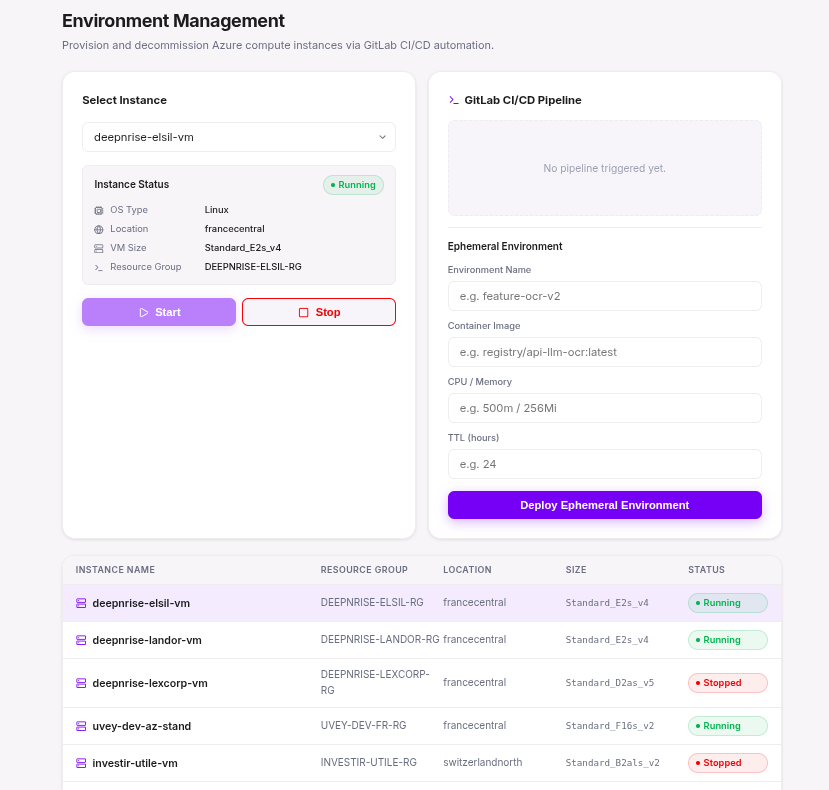
\includegraphics[width=\textwidth]{fig_vm_control}
  \caption{Module VM Control de l'\ac{IDP}~\cite{azure2023aks}}
  \label{fig:vm_control}
\end{figure}

\section*{Conclusion}
\addcontentsline{toc}{section}{Conclusion}

\noindent Ce chapitre a présenté en détails la migration vers Azure et la mise en œuvre de l'infrastructure cloud qui constitue le socle de la plateforme d'ingénierie d'Uvey. L'approche \ac{IaC} strictement définie via Terraform permet de disposer d'une infrastructure reproductible, traçable et entièrement automatisée, dans laquelle chaque élément est codifié, documenté et auditable. Le déploiement de trois clusters \ac{AKS} spécifiques garantit une isolation entre les environnements et limite l'impact d'un incident à un seul cluster. L'authentification Zero-Trust via Managed Identities élimine les problèmes liés aux secrets statiques. La migration d'Ingress NGINX vers l'Application Gateway et \ac{AGIC} améliore la sécurité, la fiabilité et les performances des accès. Enfin, la migration de la base de données PostgreSQL s'est déroulée avec succès, sans perte de données ni interruption de service, avec un chiffrement des données garanti tout au long du processus.

Le chapitre suivant traite de la stratégie de déploiement des applications et des pipelines CI/CD mis en œuvre.

\chapter{Déploiement et Gestion des Applications}
\label{chap:deploiement}

\section*{Introduction}
\addcontentsline{toc}{section}{Introduction}

\noindent Ce chapitre décrit en détail la stratégie de déploiement mise en œuvre chez Uvey.
La stratégie complète repose sur l'automatisation via des pipelines \textbf{GitLab \ac{CI/CD}}
et la réconciliation continue avec \textbf{ArgoCD} suivant le paradigme \textbf{GitOps}.
L'adoption d'une telle stratégie implique un changement majeur dans les pratiques de
livraison logicielle au sein de l'organisation : là où les déploiements étaient auparavant
des opérations manuelles, occasionnelles et sujettes aux erreurs, ils deviennent des
opérations entièrement automatisées, fréquentes et traçables.

\medskip

\noindent Ce chapitre commence par décrire la conception du pipeline \textbf{\ac{CI/CD}}, la
stratégie \textbf{GitOps} ainsi que l'utilisation des \textbf{Helm Charts} dans ArgoCD.
Il décrit ensuite l'intégration du flux de déploiement au sein de l'\ac{IDP}, puis
présente un scénario de diagnostic d'incidents afin de mettre en évidence les bénéfices
opérationnels de la plateforme. Enfin, les métriques de performance avant et après la
mise en œuvre du projet sont présentées.

\section{Gestion des déploiements avec ArgoCD}
\label{sec:argocd}

\noindent \tech{ArgoCD}~\cite{argocd2023docs} est utilisé pour les processus de livraison continue dans le cadre du paradigme GitOps, et s'exécute dans le cluster d'automatisation. Il constitue le cœur opérationnel de la déclaration des ressources Kubernetes, en assurant en temps réel la cohérence entre l'état défini dans les dépôts Git et les ressources Kubernetes déployées dans les trois clusters \ac{AKS}. À la différence des pipelines \ac{CI/CD} classiques, dans lesquels le processus déclenche activement l'application des changements au cluster, ArgoCD fonctionne selon un modèle \textit{pull} : il surveille en permanence l'état des ressources Kubernetes et les met à jour dès que l'état observé diverge de l'état déclaré. Sur le plan de la sécurité, cette approche présente l'avantage majeur d'éliminer tout accès direct aux \ac{API} des clusters de production depuis les pipelines \ac{CI/CD} externes. Toute tentative de modification manuelle d'une ressource Kubernetes est détectée et corrigée conformément à la stratégie de synchronisation définie. La Figure~\ref{fig:argocd_architecture} illustre cette architecture GitOps, en faisant apparaître le modèle \textit{pull} d'ArgoCD, les flux de synchronisation entre le dépôt Git et les trois clusters \ac{AKS}, ainsi que l'isolation complète des pipelines vis-à-vis des \ac{API} des clusters de production.

\begin{figure}[H]
  \centering
  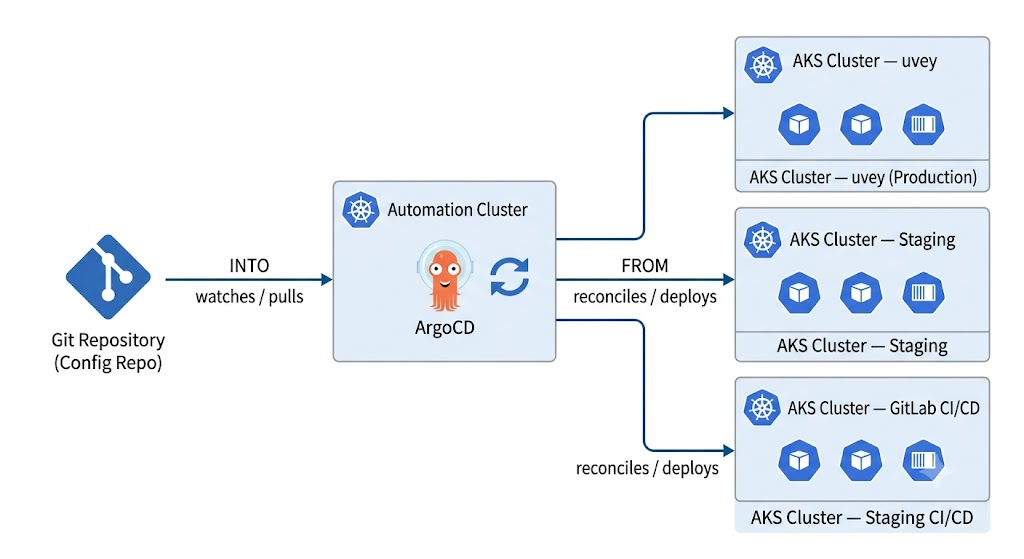
\includegraphics[width=\textwidth]{fig_argocd_architecture}
  \caption{Architecture GitOps avec ArgoCD --- synchronisation AKS~\cite{argocd2023docs}}
  \label{fig:argocd_architecture}
\end{figure}

La Figure~\ref{fig:argocd_ui} présente l'interface ArgoCD telle qu'elle apparaît en production chez Uvey, exposant pour chaque application son statut de synchronisation (\textit{Synced} / \textit{OutOfSync}), son état de santé (\textit{Healthy} / \textit{Degraded}) et le dernier commit Git appliqué.

\begin{figure}[H]
  \centering
  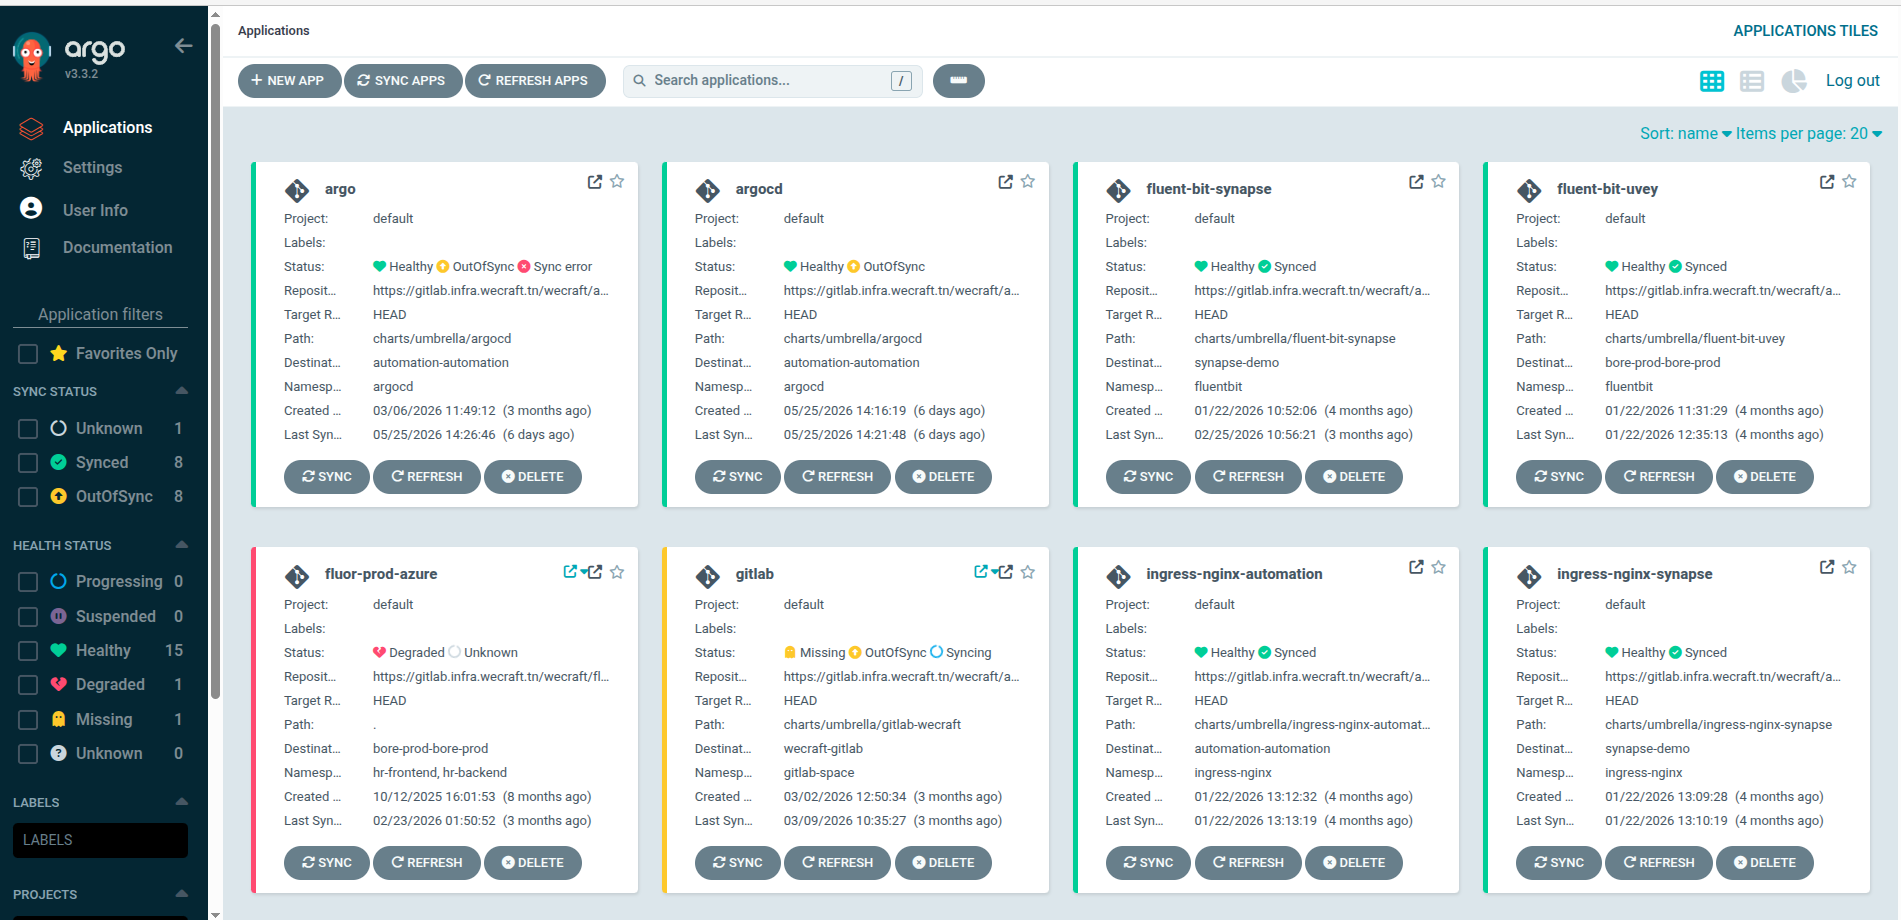
\includegraphics[width=\textwidth]{fig_argocd_ui}
  \caption{Interface ArgoCD --- statuts de synchronisation des applications~\cite{argocd2023docs}}
  \label{fig:argocd_ui}
\end{figure}

\section{Migration de la base de données PostgreSQL}
\label{sec:migration_db}

\noindent La base de données source, hébergée sur \ac{GCP}, a été transférée vers une instance Azure Database for PostgreSQL Flexible Server~\cite{azure2023postgres}. Le choix du \textit{Flexible Server} plutôt que du \textit{Single Server} s'est imposé pour plusieurs raisons : la flexibilité de paramétrage (configuration PostgreSQL entièrement personnalisable), la planification de la fenêtre de maintenance, et la possibilité d'une haute disponibilité avec un réplica de sauvegarde dans une zone de disponibilité distincte, comme le montre le tableau~\ref{tab:postgres_comparaison}.

\vspace{0.4cm}
\begin{table}[H]
  \centering
  \renewcommand{\arraystretch}{1.3}
  \begin{tabularx}{\textwidth}{L{4.5cm} L{4.5cm} L{4.5cm}}
    \toprule
    \rowcolor{uveylight}
    \textbf{Critère} & \textbf{Flexible Server} & \textbf{Single Server} \\
    \midrule
    Paramètres PostgreSQL  & Entièrement personnalisables & Limités \\
    Haute disponibilité    & Réplica en zone distincte (ZRS) & Réplica dans la même zone \\
    Fenêtre de maintenance & Planifiable par l'utilisateur & Imposée par Azure \\
    Intégration VNet       & Native (Private Endpoint) & Via règles de pare-feu \\
    Versions PG supportées & 11, 12, 13, 14, 15, 16 & 9.5 à 11 uniquement \\
    Statut produit         & Actif (recommandé par Azure) & Déprécié (retrait 2025) \\
    \textbf{Choix}         & \textbf{Retenu} & Non retenu \\
    \bottomrule
  \end{tabularx}
  \caption{Comparaison Azure PostgreSQL Flexible Server vs Single Server}
  \label{tab:postgres_comparaison}
\end{table}

\noindent La migration a été réalisée de manière sécurisée et entièrement automatisée selon les étapes suivantes :

\begin{itemize}
    \item Export de la base de données source à l'aide de \texttt{pg\_dump} avec compression parallèle afin de réduire le volume des données transférées ;

    \item Transfert du fichier d'export vers un bucket \acf{GCS} bénéficiant d'un chiffrement au repos basé sur l'algorithme AES-256 ;

    \item Provisionnement automatique d'un bastion temporaire sur Azure via Terraform, jouant le rôle de passerelle sécurisée entre les environnements \ac{GCP} et Azure ;

    \item Restauration de la base de données dans Azure PostgreSQL Flexible Server via \texttt{pg\_restore} en mode parallèle (\texttt{-j 4}), permettant l'exécution simultanée de plusieurs tâches de restauration et réduisant significativement la durée de l'opération ;

    \item Validation de l'intégrité des données restaurées par comparaison des checksums et des statistiques entre la base source et la base cible ;

    \item Suppression automatique du bastion temporaire après validation, afin de minimiser la surface d'exposition de l'infrastructure.
\end{itemize}

\noindent Tout au long du processus, la sécurité des données a été préservée grâce au maintien du chiffrement en transit via TLS 1.3 et au chiffrement au repos via AES-256. Les données n'ont à aucun moment transité sur Internet sous une forme non chiffrée, garantissant ainsi la confidentialité et l'intégrité des informations durant toute l'opération de migration. La Figure~\ref{fig:migration_db} représente l'enchaînement complet des étapes de migration, depuis l'export \texttt{pg\_dump} sur \ac{GCP} jusqu'à la restauration sur Azure Flexible Server via le bastion temporaire, en indiquant pour chaque étape le mécanisme de chiffrement en vigueur.

\begin{figure}[H]
  \centering
  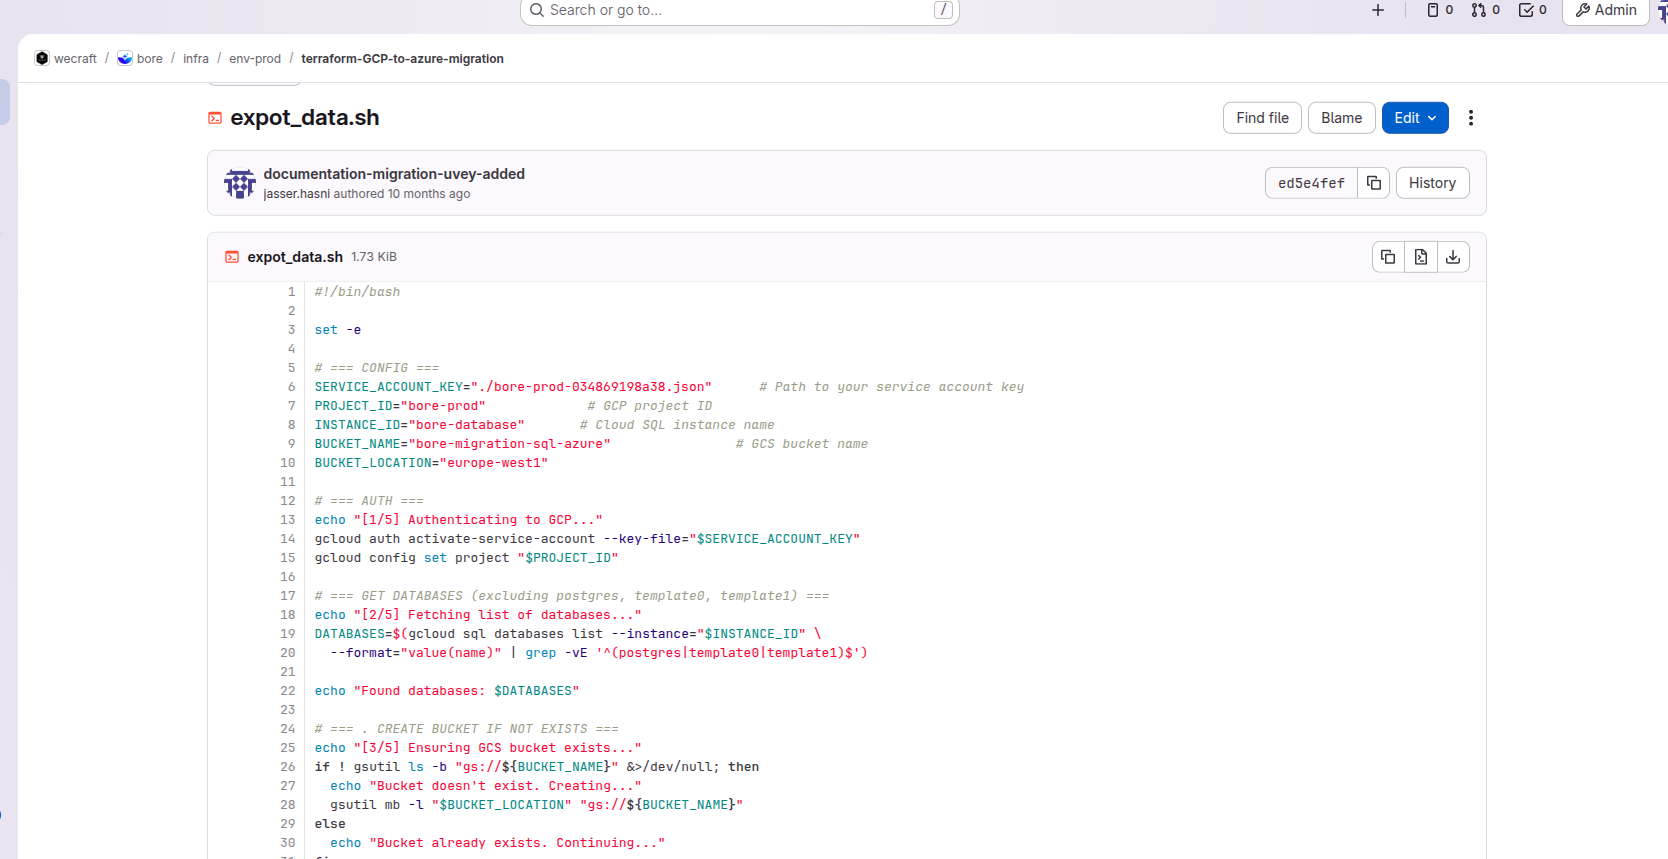
\includegraphics[width=\textwidth]{fig_migration_db}
  \caption{Processus de migration PostgreSQL de \ac{GCP} vers Azure~\cite{azure2023postgres}}
  \label{fig:migration_db}
\end{figure}


\section{Stratégie de déploiement et pipeline CI/CD}
\label{sec:pipeline_cicd}

\noindent Cette section présente la stratégie de déploiement adoptée, en distinguant l'environnement de développement, où la rapidité de feedback est prioritaire, de l'environnement de production, où la fiabilité et la traçabilité sont essentielles.

\subsection{Environnement de développement}

La gestion automatisée des déploiements est devenue l'élément central du processus de développement~\cite{forsgren2018accelerate}. Les pipelines d'\acf{CI/CD} s'exécutent sur l'infrastructure GitLab d'Uvey et couvrent l'intégralité du cycle de vie du microservice : compilation du code source, exécution des tests unitaires et d'intégration, contrôle de la qualité du code par analyse statique, construction de l'image Docker, publication au registre de conteneurs, et déclenchement de l'automatisme de déploiement via le flux GitOps. Chaque étape du pipeline est atomique et produit un rapport d'exécution garantissant une traçabilité complète. La Figure~\ref{fig:cicd_pipeline} présente le pipeline \ac{CI/CD} complet, en déroulant chacune de ces étapes depuis le commit initial jusqu'au déploiement en production, et en faisant apparaître les points de contrôle qualité et les artefacts produits à chaque stage.

\begin{figure}[H]
  \centering
  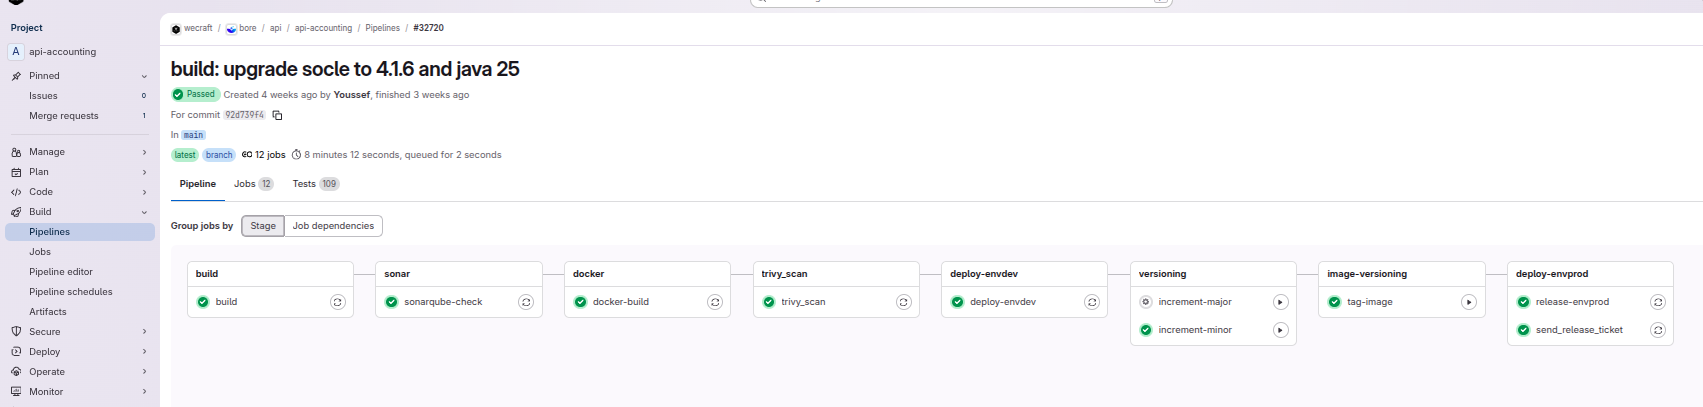
\includegraphics[width=\textwidth]{fig_cicd_pipeline}
  \caption{Pipeline \ac{CI/CD} complet --- du commit au déploiement en production~\cite{argocd2023docs}}
  \label{fig:cicd_pipeline}
\end{figure}

À chaque push sur la branche \texttt{main}, le pipeline crée une image Docker identifiée par le SHA du commit et la déploie dans l'environnement de développement, qui utilise \tech{Docker Compose}~\cite{docker2023compose}. Cet environnement est composé de plusieurs conteneurs issus de la même image. Il fournit au développeur un cycle de feedback rapide, avec des temps de déploiement inférieurs à deux minutes. L'utilisation du SHA du commit comme étiquette garantit l'immuabilité et l'unicité de chaque build.

\subsection{Environnement de production}

Pour le passage en production, la mise en œuvre suit le modèle GitOps : l'image Docker est étiquetée avec un tag immuable basé sur le SHA du commit, publiée sur le \acf{GCR}, puis le pipeline met à jour automatiquement le manifeste Kubernetes dans le dépôt de configuration. ArgoCD détecte alors les modifications et resynchronise automatiquement le cluster \ac{AKS} via une mise à jour en \textit{rolling update}, sans interruption de service.

Le mécanisme de \textit{rolling update} garantit qu'à aucun moment l'ensemble des réplicas d'un déploiement ne sont arrêtés simultanément : les nouveaux pods sont démarrés et validés par les \textit{readiness probes} avant que les anciens ne soient arrêtés. Ainsi, aucune interruption de service n'est perceptible par les utilisateurs d'Uvey lors du déploiement. En cas d'anomalie détectée par les readiness probes, ArgoCD effectue automatiquement un rollback vers la version précédente du déploiement. La Figure~\ref{fig:gitops_pipeline} illustre l'étape de mise à jour automatique du manifeste GitOps au sein du pipeline, montrant comment le tag d'image issu du build est injecté dans le fichier \texttt{deployment.yaml} du dépôt de configurations avant d'être poussé par le pipeline.

\begin{figure}[H]
  \centering
  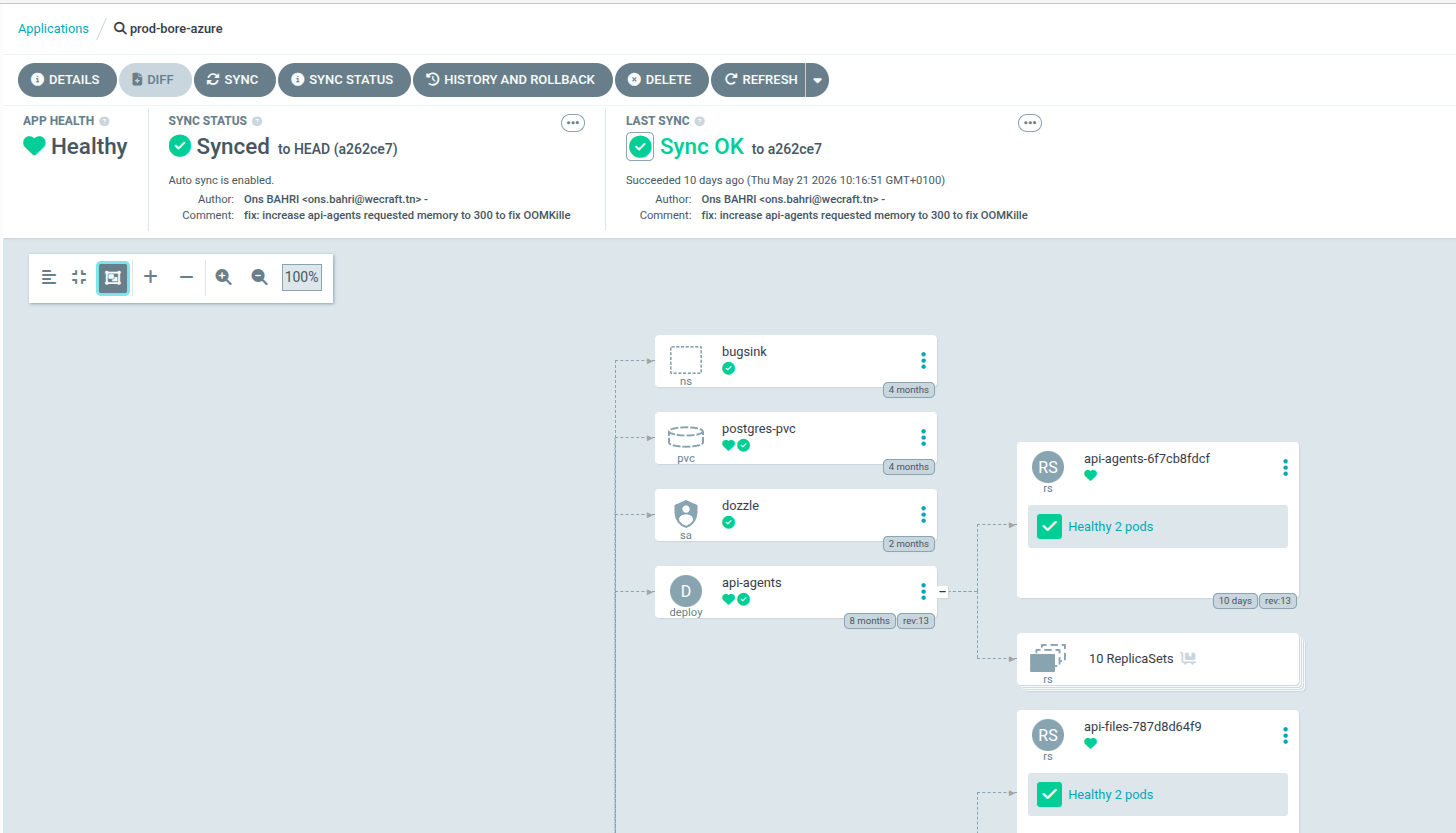
\includegraphics[width=0.88\textwidth]{fig_gitops_pipeline}
  \caption{Mise à jour automatique du manifeste GitOps --- extrait \ac{CI/CD}~\cite{weaveworks2021gitops}}
  \label{fig:gitops_pipeline}
\end{figure}

\section{Approche GitOps avec ArgoCD et gestion des Helm Charts}
\label{sec:gitops_argocd}

\noindent Cette section détaille le fonctionnement du paradigme GitOps tel qu'il est mis en œuvre avec ArgoCD, ainsi que la gestion des Helm Charts dans ce contexte.

\subsection{Réconciliation continue avec ArgoCD}

\noindent Avant de retenir GitOps comme paradigme central, plusieurs approches de gestion des déploiements ont été évaluées au regard des exigences de traçabilité, de sécurité et d'auditabilité du projet, comme le résume le tableau~\ref{tab:deploy_comparaison}.

\begin{table}[H]
  \centering
  \renewcommand{\arraystretch}{1.3}
  \begin{tabularx}{\textwidth}{L{3.5cm} L{3.5cm} L{3.5cm} L{3cm}}
    \toprule
    \rowcolor{uveylight}
    \textbf{Critère} & \textbf{GitOps (ArgoCD)} & \textbf{\ac{CI/CD} push classique} & \textbf{Scripts manuels} \\
    \midrule
    Traçabilité       & Complète (Git history) & Partielle (logs CI) & Inexistante \\
    Rollback          & \texttt{git revert} immédiat & Rebuild du pipeline & Manuel, risqué \\
    Accès cluster     & Aucun accès externe requis & Accès direct cluster & Accès direct cluster \\
    Dérive config.    & Détectée et corrigée auto. & Non détectée & Non détectée \\
    Auditabilité      & Totale & Partielle & Nulle \\
    Réconciliation    & Continue et automatique & À chaque pipeline & Inexistante \\
    \textbf{Choix}    & \textbf{Retenu} & Non retenu & Non retenu \\
    \bottomrule
  \end{tabularx}
  \caption{Comparaison des approches de déploiement et gestion de configuration}
  \label{tab:deploy_comparaison}
\end{table}

\noindent L'approche \textbf{GitOps}~\cite{weaveworks2021gitops} repose sur le postulat que le dépôt Git constitue l'unique et immuable source de vérité concernant l'état souhaité du système. En pratique, les pipelines se contentent de pousser des commits dans Git, tandis qu'ArgoCD, exécuté depuis le cluster lui-même, se charge de réconcilier l'état effectif avec l'état déclaré. Cette inversion des rôles entre pipelines et clusters offre plusieurs avantages significatifs : \textbf{traçabilité complète} de chaque modification via le commit Git horodaté et signé, \textbf{rollback} simplifié par une commande \texttt{git revert}, \textbf{sécurité renforcée} puisque les pipelines n'ont jamais besoin d'un accès direct au cluster de production, et \textbf{auditabilité} totale. En cas de divergence --- par exemple, si un opérateur modifie manuellement une ressource dans le cluster --- celle-ci est aussitôt détectée et corrigée conformément à la stratégie de synchronisation définie, garantissant que l'état effectif reste en permanence aligné sur l'état déclaré dans Git. La Figure~\ref{fig:gitops_reconciliation} représente ce modèle de réconciliation continue, en illustrant la boucle de contrôle par laquelle ArgoCD compare périodiquement l'état observé dans le cluster à l'état déclaré dans Git et déclenche une resynchronisation dès qu'une divergence est détectée.

\begin{figure}[H]
  \centering
  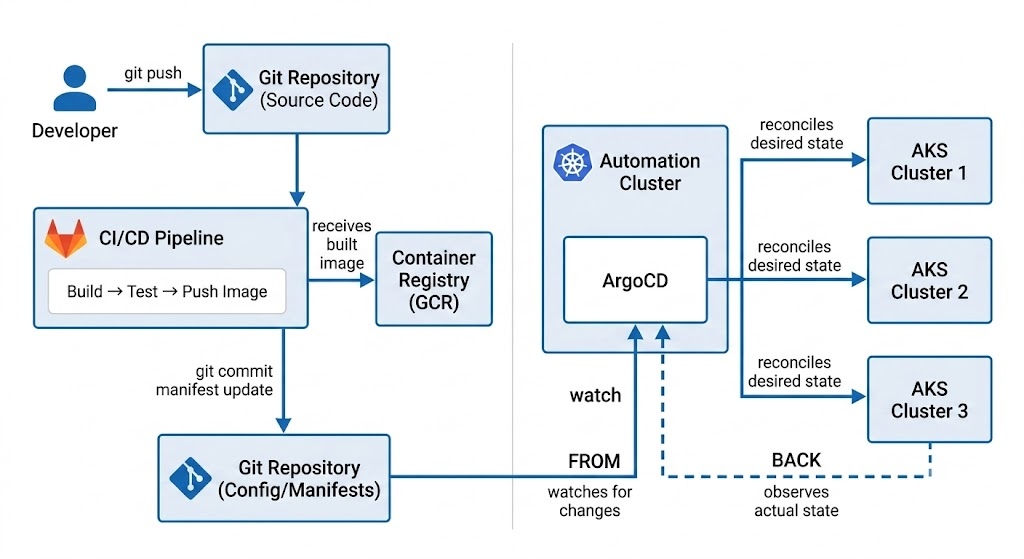
\includegraphics[width=\textwidth]{fig_gitops_reconciliation}
  \caption{Modèle de réconciliation GitOps avec ArgoCD~\cite{argocd2023docs}}
  \label{fig:gitops_reconciliation}
\end{figure}

\subsection{Gestion des Helm Charts}

\noindent La gestion des charts Helm~\cite{helm2023docs} via ArgoCD permet de résoudre le problème de dérive de configuration, en soumettant chaque chart au mécanisme de réconciliation GitOps. Avant l'adoption d'ArgoCD, les mises à jour des charts Helm s'effectuaient manuellement via la commande \texttt{helm upgrade}, ce qui engendrait des dérives de configuration non détectées, empêchait tout rollback fiable et créait un risque de désynchronisation entre les valeurs réellement appliquées sur le cluster et celles présentes dans le dépôt Git. ArgoCD surveille en permanence les dépôts Git où sont stockées les valeurs de configuration des charts et identifie automatiquement toute divergence entre l'état déclaratif et l'état observé. Les applications ArgoCD encapsulent chaque chart Helm avec ses propres valeurs de configuration, simplifiant ainsi la gestion de composants complexes tels que la stack de monitoring ou le gestionnaire de secrets. La Figure~\ref{fig:helm_argocd} illustre comment une application ArgoCD encapsule un chart Helm avec son fichier de valeurs dédié, permettant à ArgoCD de détecter toute divergence entre les valeurs déclarées dans Git et celles effectivement appliquées sur le cluster.

\begin{figure}[H]
  \centering
  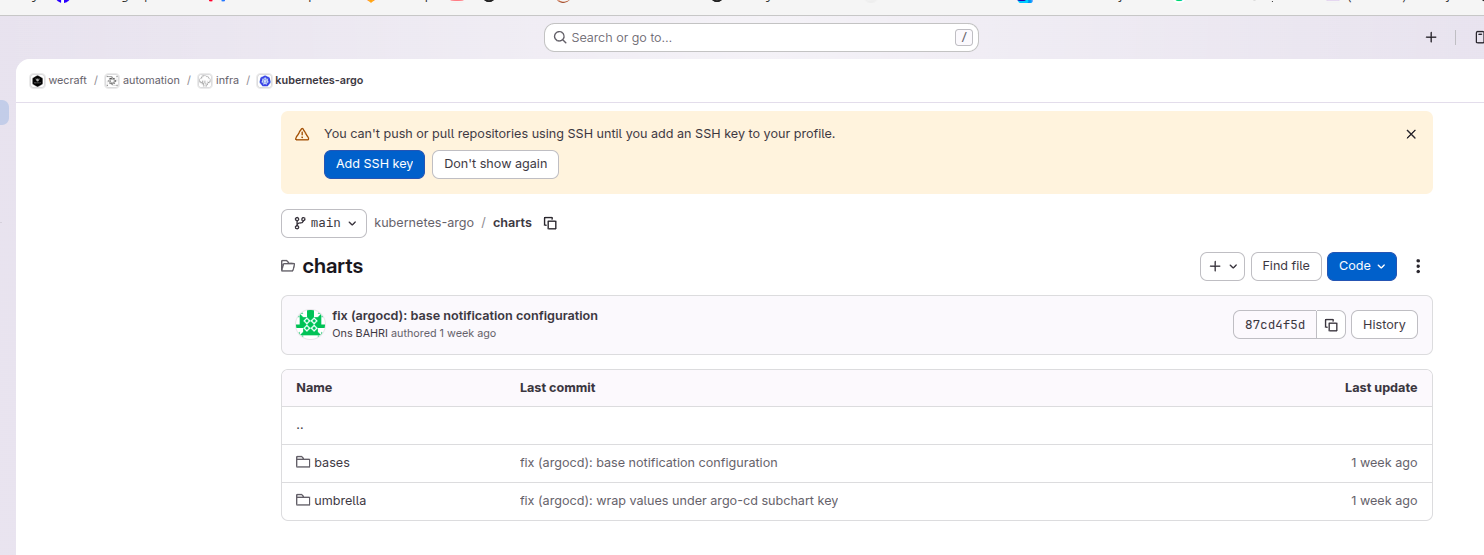
\includegraphics[width=0.88\textwidth]{fig_helm_argocd}
  \caption{Gestion des Helm Charts via les Applications ArgoCD~\cite{argocd2023docs}}
  \label{fig:helm_argocd}
\end{figure}

La Figure~\ref{fig:argocd_sync_policy} présente la politique de synchronisation configurée pour la stack de monitoring, détaillant les options \textit{selfHeal} et \textit{automated} qui assurent la correction automatique de toute dérive sans intervention manuelle.

\begin{figure}[H]
  \centering
  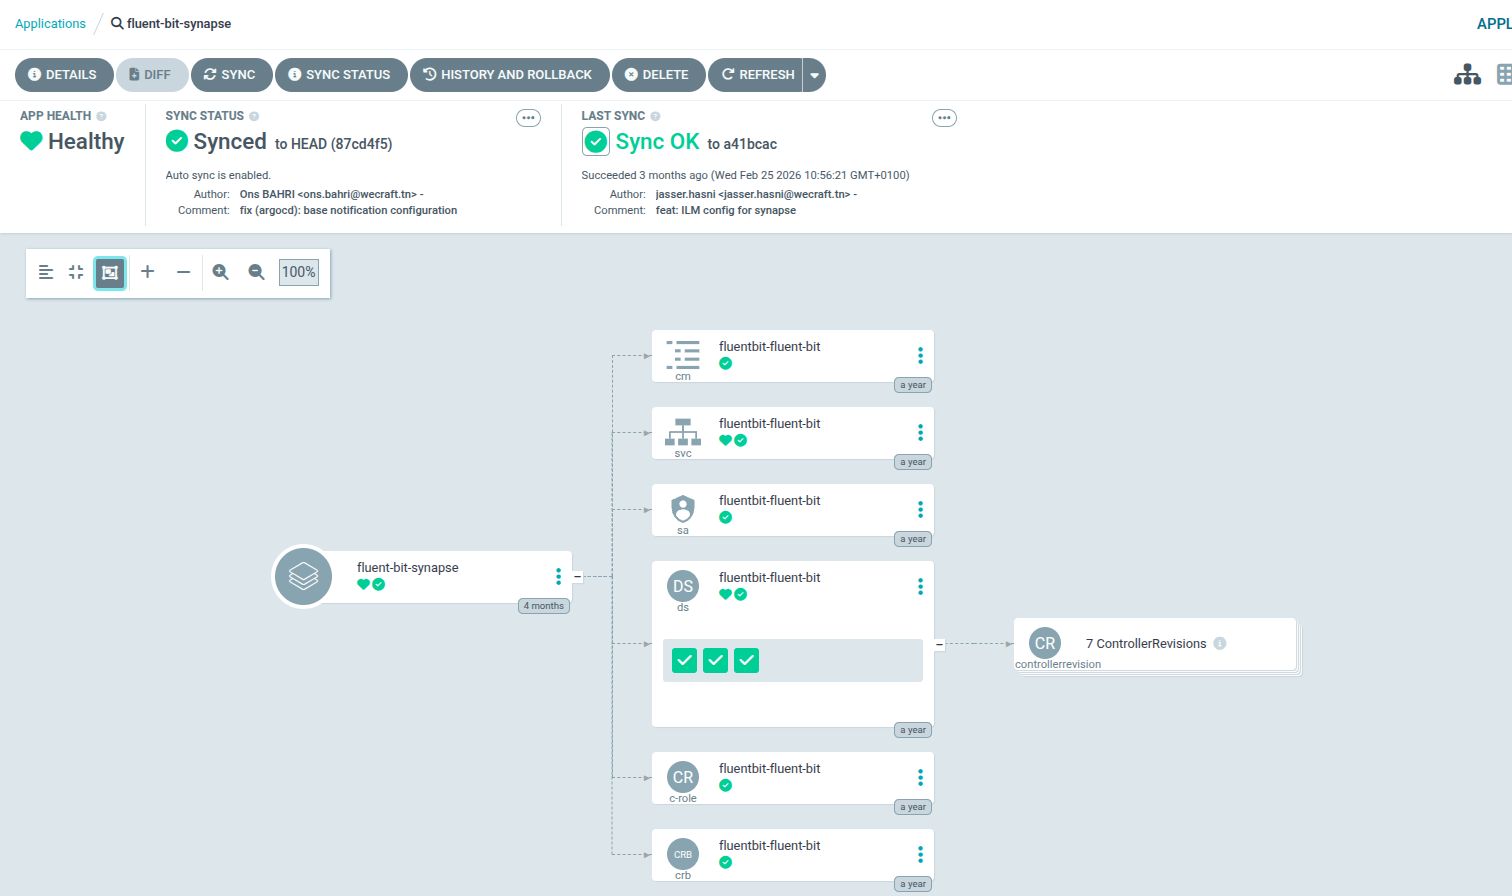
\includegraphics[width=0.88\textwidth]{fig_argocd_sync_policy}
  \caption{Politique de synchronisation ArgoCD pour la stack de monitoring~\cite{argocd2023docs}}
  \label{fig:argocd_sync_policy}
\end{figure}

\section{Scénario de déploiement de bout en bout}
\label{sec:use_case_deploy}

\noindent Ce scénario illustre le flux complet de déploiement d'une mise à jour du microservice \texttt{api-accounting} de la version \texttt{v2.3.1} vers la version \texttt{v2.4.0}. Ce cas d'usage est représentatif de la grande majorité des opérations de mise en production quotidiennes chez Uvey, et illustre concrètement comment les différentes briques technologiques --- GitLab \ac{CI/CD}, Docker, ArgoCD, \ac{AKS} et l'\ac{IDP} --- s'articulent en un flux cohérent, traçable et réversible :

\begin{enumerate}
  \item Le développeur pousse ses modifications sur la branche \texttt{main} du dépôt \texttt{api-accounting}.
  \item Le pipeline GitLab \ac{CI/CD} se déclenche automatiquement : build, tests unitaires, tests d'intégration.
  \item En cas de succès, l'image Docker \texttt{gcr.io/uvey/api-accounting:v2.4.0} est publiée sur \ac{GCR}.
  \item Le pipeline met à jour le manifeste \texttt{deployment.yaml} dans le dépôt de configurations.
  \item ArgoCD détecte la modification dans Git et synchronise automatiquement le cluster \ac{AKS}.
  \item Le déploiement en \textit{rolling update} est effectué sans interruption de service.
  \item Le développeur visualise le statut du déploiement depuis l'\ac{IDP} en temps réel.
\end{enumerate}

\noindent En cas d'échec à l'une des étapes, le flux est interrompu immédiatement et une alerte est envoyée à l'équipe via le canal de communication dédié. La correction de l'anomalie et le redémarrage du pipeline suffisent à reprendre le cours des opérations sans intervention manuelle sur le cluster. En cas de problème constaté après le déploiement, un \texttt{git revert} sur le dépôt de configurations suffit à déclencher un rollback automatique par ArgoCD. La Figure~\ref{fig:gitlab_pipeline} présente le résultat d'un tel déploiement réussi dans l'interface GitLab, avec l'ensemble des stages du pipeline au vert et le tag \texttt{v2.4.0} correctement publié sur le registre de conteneurs.

\begin{figure}[H]
  \centering
  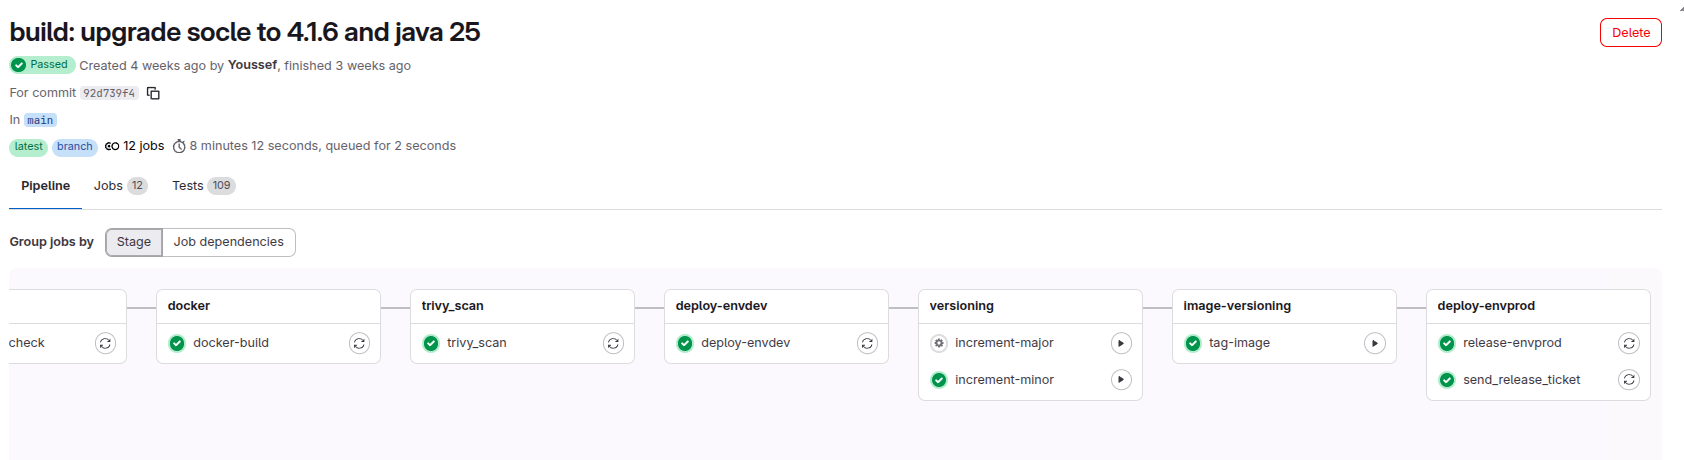
\includegraphics[width=\textwidth]{fig_gitlab_pipeline_success}
  \caption{Déploiement réussi de \texttt{api-accounting} v2.4.0~\cite{argocd2023docs}}
  \label{fig:gitlab_pipeline}
\end{figure}

\section{Intégration des déploiements dans l'IDP}
\label{sec:deploy_idp}

\noindent L'intégration du flux de déploiement dans l'\ac{IDP} est la conclusion naturelle de l'approche de centralisation. Sans cette intégration, les développeurs devraient naviguer entre plusieurs interfaces --- GitLab pour le pipeline, ArgoCD pour suivre l'état du déploiement, Grafana pour analyser la santé des services --- pour disposer d'une vision d'ensemble de leur microservice. L'\ac{IDP} centralise toutes ces informations dans une vue par service unique. Dans le \textit{Software Catalog}, chaque microservice est enrichi de liens directs vers ses pipelines courants ou récents sur GitLab, de son état de synchronisation ArgoCD avec un aperçu des ressources déployées, et des métriques de santé issues de Prometheus. Ces liens sont créés automatiquement à partir des données déclaratives du fichier \texttt{catalog-info.yaml} de chaque service : le simple ajout d'un service au catalogue suffit à lui attribuer l'ensemble de ces intégrations. La Figure~\ref{fig:idp_service_detail} présente la vue détaillée d'un microservice dans l'\ac{IDP}, faisant apparaître en un seul écran son statut ArgoCD, ses pipelines GitLab récents, ses métriques Prometheus et ses liens pré-filtrés vers Grafana et Kibana.

\begin{figure}[H]
  \centering
  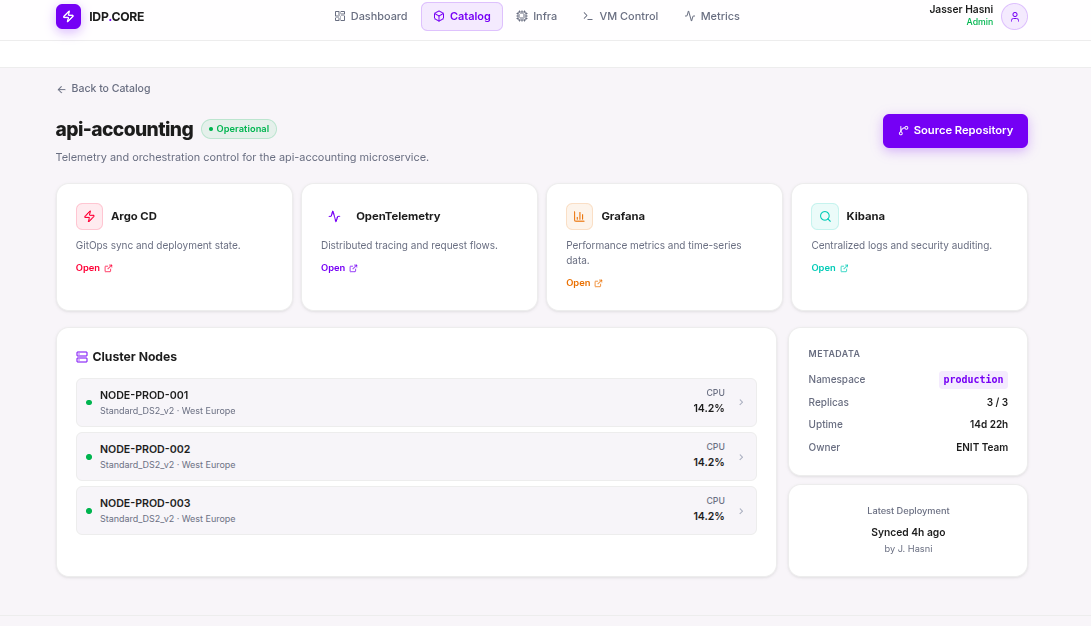
\includegraphics[width=\textwidth]{fig_idp_service_detail}
  \caption{Vue détaillée d'un microservice dans l'\ac{IDP} avec ses liens profonds~\cite{backstage2023catalog}}
  \label{fig:idp_service_detail}
\end{figure}

\section{Scénario de diagnostic d'incident}
\label{sec:use_case_monitoring}

\noindent Ce scénario illustre le diagnostic d'un incident de performance sur le service \texttt{api-llm-ocr}, détecté via les alertes Grafana~\cite{prometheus2023docs}. Il met en évidence la manière dont l'\ac{IDP} permet au développeur de passer de l'alerte à la correction sans quitter une interface centralisée, et sans avoir à connaître par cœur les URLs de chaque outil d'observabilité ou les filtres à appliquer pour isoler les données du service concerné :

\begin{enumerate}
  \item Grafana déclenche une alerte : la latence P95 du service \texttt{api-llm-ocr} dépasse 3 secondes.
  \item Le développeur reçoit une notification et accède directement à l'\ac{IDP}.
  \item Depuis la page du service dans le \textit{Software Catalog}, il clique sur le lien Grafana pré-filtré.
  \item Il identifie une corrélation entre la montée de latence et un \textit{OOMKill} sur un pod.
  \item Il consulte les logs Kibana via le lien pré-filtré pour confirmer l'erreur mémoire.
  \item Il ajuste les \textit{resource limits} dans le manifeste Git ; ArgoCD déploie automatiquement la correction.
\end{enumerate}

\noindent Sans l'\ac{IDP}, ce même diagnostic aurait nécessité d'ouvrir successivement Grafana, Kibana et l'interface ArgoCD, d'appliquer manuellement les filtres appropriés sur chaque outil, et de corréler des informations issues de sources hétérogènes. Le gain de temps sur ce type d'opération, répété plusieurs fois par semaine à l'échelle de l'ensemble des équipes, représente un bénéfice opérationnel significatif et mesurable.

\section{Métriques de performance}
\label{sec:resultats}

\noindent Les améliorations constatées à l'issue de la mise en œuvre de l'\ac{IDP} et de l'infrastructure Azure sont synthétisées dans le tableau~\ref{tab:resultats}. Ces indicateurs ont été obtenus sur une période représentative, avant et après la mise en production de la solution, à partir des données issues des pipelines GitLab, des logs ArgoCD et des tableaux de bord Grafana. Ils permettent de vérifier quantitativement les gains évoqués lors de l'analyse de la problématique : amélioration de la vitesse de provisionnement des environnements de test, réduction du temps de déploiement en production et diminution du \ac{MTTR}.

\begin{table}[H]
  \centering
  \renewcommand{\arraystretch}{1.4}
  \begin{tabularx}{\textwidth}{L{6cm} C{3.5cm} C{3.5cm}}
    \toprule
    \rowcolor{uveylight}
    \textbf{Métrique} & \textbf{Avant} & \textbf{Après} \\
    \midrule
    Temps de création d'un environnement de test & $\sim$30 min (manuel) & $\sim$5 min (self-service) \\
    Temps de déploiement en production & $\sim$20 min & $\sim$8 min \\
    Nombre d'outils pour un diagnostic & 4--5 outils & 1 interface (\ac{IDP}) \\
    Temps moyen de résolution d'incident (\ac{MTTR}) & $\sim$45 min & $\sim$20 min \\
    Dérives de configuration & Non contrôlées (manuel) & Automatique (ArgoCD) \\
    Traçabilité des déploiements & Partielle & Complète (Git log) \\
    \bottomrule
  \end{tabularx}
  \caption{Métriques d'amélioration --- avant et après le projet~\cite{dora2023}}
  \label{tab:resultats}
\end{table}

\section*{Conclusion}
\addcontentsline{toc}{section}{Conclusion}

Ce chapitre a détaillé la stratégie de déploiement adoptée par Uvey. Les pipelines GitLab \ac{CI/CD} couvrent l'intégralité du cycle de vie de chaque microservice, depuis la compilation du code source jusqu'à la construction et la publication de l'image Docker. L'approche GitOps avec ArgoCD garantit des déploiements 100\% traçables, réversibles et sans interruption de service via le \textit{rolling update}. Elle permet également d'éliminer les risques liés à un accès direct aux clusters depuis les pipelines. La gestion des Helm Charts via ArgoCD prévient les dérives de configuration causées par des déploiements manuels. L'intégration de l'ensemble de ces flux au sein de l'\ac{IDP} consolide l'expérience développeur et élimine le besoin de naviguer entre plusieurs outils. 

\textbf{Le chapitre suivant présente le déploiement de la pile d'observabilité.}

\chapter{Mise en Place de l'Observabilité}
\label{chap:observabilite}

\section*{Introduction}
\addcontentsline{toc}{section}{Introduction}

\noindent Ce chapitre présente la pile d'observabilité complète mise en place pour rendre l'infrastructure d'Uvey entièrement observable. Dans une architecture microservices distribuée, la capacité à comprendre ce qui se passe au sein du système est non seulement utile, mais essentielle à son bon fonctionnement. Un incident de production dans un contexte d'observabilité insuffisante se traduit par de longues heures de diagnostic, des clients insatisfaits et une confiance dégradée. Ce chapitre aborde successivement l'architecture générale de la pile d'observabilité, puis ses trois piliers constitutifs : la stack ELK pour la gestion des logs, Prometheus et Grafana pour le monitoring des métriques, et OpenTelemetry pour le traçage distribué.

\section{Architecture globale de l'observabilité}
\label{sec:obs_architecture}

\noindent Dans un environnement microservices, l'observabilité n'est pas un confort : c'est une condition sine qua non pour opérer efficacement et réagir rapidement au sein d'un système distribué. Un système observable se caractérise par la possibilité de déterminer son état interne à partir de ses sorties externes, sans nécessiter l'ajout d'un mécanisme de débogage spécifique pour chaque nouveau type de problème. La pile d'observabilité déployée couvre les trois piliers fondamentaux recommandés par les experts du domaine~\cite{sridharan2018distributed} : \textbf{logs}, \textbf{métriques} et \textbf{traçage distribué}. Ces trois piliers ont chacun leur utilité propre : les métriques signalent l'apparition d'un problème, les logs fournissent le contexte, et les traces indiquent le chemin emprunté par une requête pour identifier le composant défaillant. La Figure~\ref{fig:obs_architecture} représente l'architecture globale de cette pile, faisant apparaître les flux de données entre les agents de collecte, les pipelines de traitement et les backends de stockage pour chacun des trois piliers.

\begin{figure}[H]
  \centering
  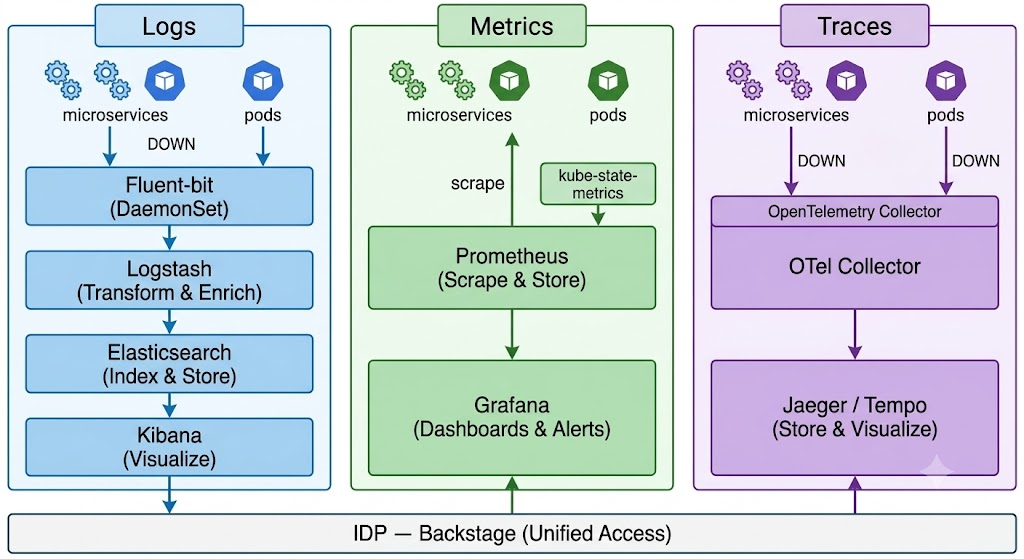
\includegraphics[width=\textwidth]{fig_observabilite_architecture}
  \caption{Architecture de la pile d'observabilité --- logs, métriques et traces~\cite{sridharan2018distributed}}
  \label{fig:obs_architecture}
\end{figure}

\begin{table}[htbp]
  \centering
  \renewcommand{\arraystretch}{1.3}
  \begin{tabularx}{\textwidth}{L{3cm} L{4cm} L{7cm}}
    \toprule
    \rowcolor{uveylight}
    \textbf{Pilier} & \textbf{Outil} & \textbf{Rôle} \\
    \midrule
    Logs & Fluent-bit & Collecte légère depuis les nœuds AKS \\
    Logs & Logstash & Transformation et enrichissement des logs \\
    Logs & Elasticsearch & Indexation et stockage des logs \\
    Logs & Kibana & Visualisation et exploration des logs \\
    \midrule
    Métriques & Prometheus & Scraping et stockage des métriques \\
    Métriques & Grafana & Visualisation et alerting \\
    Métriques & kube-state-metrics & Métriques des objets Kubernetes \\
    \midrule
    Traces & OpenTelemetry Collector & Réception et exportation des traces \\
    Traces & Tempo / Jaeger & Stockage et visualisation des traces \\
    \bottomrule
  \end{tabularx}
  \caption{Composants de la pile d'observabilité et leurs rôles}
  \label{tab:obs_components}
\end{table}

\section{Collecte des logs avec la stack ELK}
\label{sec:logs}

\noindent Cette section décrit la chaîne complète de gestion des logs, depuis leur collecte sur les nœuds \ac{AKS} jusqu'à leur visualisation dans Kibana, en passant par leur enrichissement via Logstash.

\subsection{Collecte et enrichissement avec Fluent-bit et Logstash}

\noindent Les fichiers journaux générés par l'ensemble des conteneurs sont collectés par \tech{Fluent-bit}~\cite{fluentbit2023docs}, un agent minimaliste déployé en mode \textit{DaemonSet} sur chaque nœud \ac{AKS}. Cette architecture garantit la présence d'un agent de collecte sur chacun des nœuds du cluster. Fluent-bit a été préféré à son prédécesseur Fluentd en raison de sa faible empreinte mémoire, ce qui présente un avantage notable dans une configuration distribuée, comme le montre la comparaison du tableau~\ref{tab:fluentbit_comparaison}.

Ces données transitent ensuite vers Logstash pour être enrichies et normalisées : des métadonnées relatives à leur environnement d'origine sont ajoutées, telles que le nom du cluster, le namespace Kubernetes, le nom du pod et du microservice. Ces logs sont enfin indexés dans Elasticsearch. Cette étape est essentielle : sans normalisation, des logs bruts provenant de sources hétérogènes et de formats variés (JSON structuré, texte brut, stack traces multilignes) seraient difficiles à interroger de manière cohérente. Logstash utilise des filtres \texttt{grok} et \texttt{mutate} pour normaliser les champs des logs, rendant possible des requêtes transversales telles que : \textit{« afficher tous les logs d'erreur du service api-accounting des 30 dernières minutes »}.

\begin{table}[H]
  \centering
  \renewcommand{\arraystretch}{1.3}
  \begin{tabularx}{\textwidth}{L{4cm} C{4cm} C{4cm}}
    \toprule
    \rowcolor{uveylight}
    \textbf{Critère} & \textbf{Fluent-bit} & \textbf{Fluentd} \\
    \midrule
    Consommation mémoire & $\sim$450 KB & $\sim$40 MB \\
    Consommation CPU      & Très faible & Modérée \\
    Plugins disponibles   & Essentiels  & Très nombreux (600+) \\
    Modèle de déploiement & DaemonSet (nœud) & DaemonSet ou agrégateur \\
    Langage               & C           & Ruby \\
    Cas d'usage optimal   & Collecte légère sur nœuds & Pipeline de transformation complexe \\
    \textbf{Choix}        & \textbf{Retenu} & Non retenu \\
    \bottomrule
  \end{tabularx}
  \caption{Comparaison Fluent-bit vs Fluentd pour la collecte des logs}
  \label{tab:fluentbit_comparaison}
\end{table}

\subsection{Indexation et visualisation avec Elasticsearch et Kibana}

\noindent Elasticsearch assure le stockage, l'indexation et la recherche des journaux disponibles dans la plateforme. Les logs sont stockés dans des index horodatés, permettant un traitement efficace de grands volumes de données et une recherche chronologique performante. Une stratégie de rétention est définie pour trouver un équilibre entre le besoin historique d'investigation, les éventuelles exigences de conformité et les contraintes de stockage de l'infrastructure.

La plateforme utilise les mécanismes d'\acf{ILM} pour assurer une transition automatique des index entre différents niveaux de stockage en fonction de leur âge et de leur fréquence d'utilisation. Les index les plus récents, consultés le plus fréquemment dans les activités de supervision et d'analyse, sont conservés en phase \textit{hot}, garantissant de hautes performances en lecture et en écriture. Lorsque la fréquence d'utilisation diminue, les données sont transférées en phase \textit{warm}, restant accessibles tout en consommant moins de ressources. La Figure~\ref{fig:kibana_dashboard} présente le tableau de bord Kibana tel qu'il est utilisé en production, permettant d'explorer et de filtrer les logs par microservice, par niveau de sévérité et par fenêtre temporelle. La Figure~\ref{fig:fluentbit_config} illustre la configuration de sortie de Fluent-bit, montrant comment les logs collectés sur les nœuds sont acheminés vers Elasticsearch avec les métadonnées de contexte Kubernetes.

\begin{figure}[H]
  \centering
  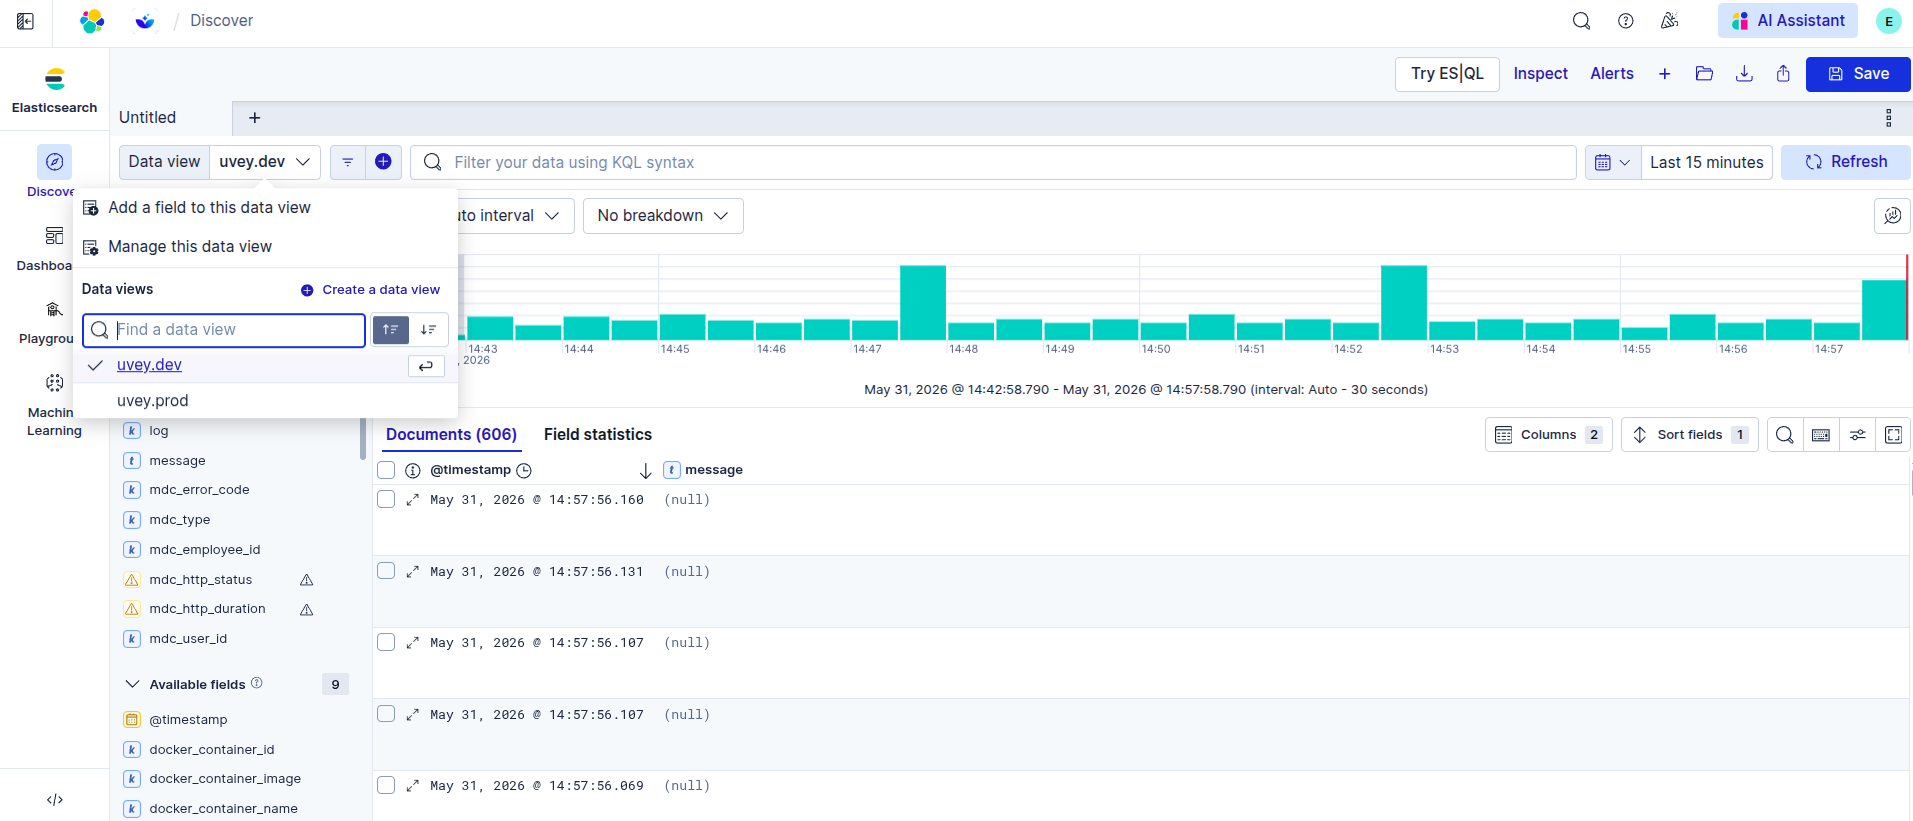
\includegraphics[width=\textwidth]{fig_kibana_dashboard}
  \caption{Tableau de bord Kibana --- exploration des logs par microservice~\cite{fluentbit2023docs}}
  \label{fig:kibana_dashboard}
\end{figure}

\begin{figure}[H]
  \centering
  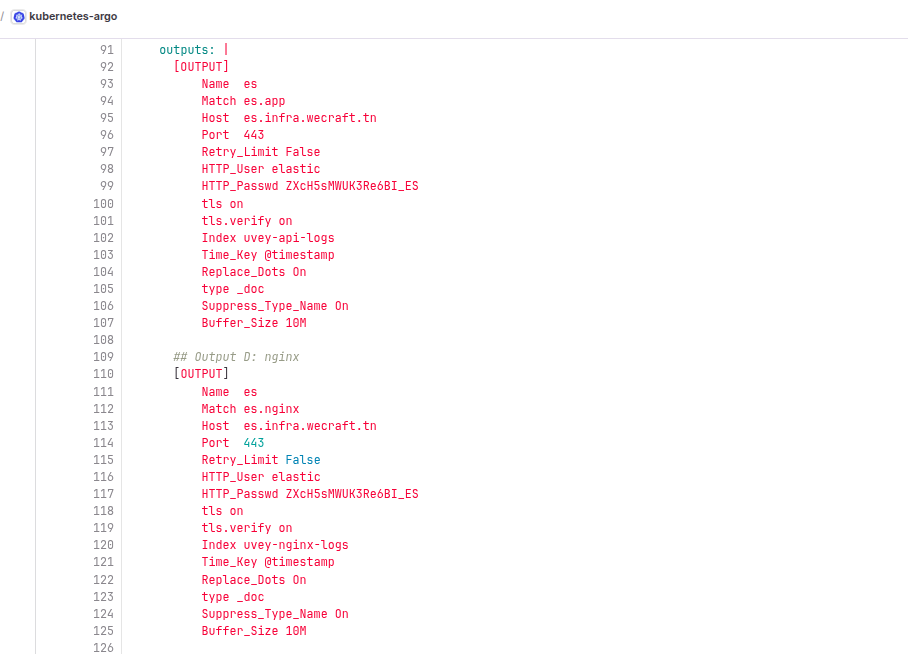
\includegraphics[width=0.88\textwidth]{fig_fluentbit_config}
  \caption{Configuration de sortie Fluent-bit vers Elasticsearch~\cite{fluentbit2023docs}}
  \label{fig:fluentbit_config}
\end{figure}

\section{Monitoring des métriques avec Prometheus et Grafana}
\label{sec:metriques}

\noindent Cette section présente la mise en place du monitoring des métriques, en décrivant d'abord la collecte et le stockage avec Prometheus, puis la visualisation et l'alerting avec Grafana.

\subsection{Collecte et stockage avec Prometheus}

\noindent Prometheus~\cite{prometheus2023docs} est installé via le chart Helm \texttt{kube-prometheus-stack}, une distribution préintégrée et paramétrable qui regroupe le serveur Prometheus, Alertmanager, kube-state-metrics et node-exporter. Le recours à cette distribution unifiée se justifie par plusieurs raisons : la cohérence des versions entre les différents modules, la présence de règles d'alertes Kubernetes par défaut fondées sur les bonnes pratiques du marché, et une réduction significative de l'effort de configuration. L'architecture de collecte de Prometheus repose sur le mode \textit{pull} : Prometheus interroge chaque microservice et composant infrastructure via leur endpoint \texttt{/metrics} à des intervalles configurables par cible. Il suffit ainsi de donner à Prometheus lui-même les permissions réseau pour accéder à ces endpoints. La comparaison avec les alternatives est présentée dans le tableau~\ref{tab:prometheus_comparaison}.

\begin{table}[H]
  \centering
  \renewcommand{\arraystretch}{1.3}
  \begin{tabularx}{\textwidth}{L{4cm} C{3.5cm} C{3.5cm} C{3cm}}
    \toprule
    \rowcolor{uveylight}
    \textbf{Critère} & \textbf{Prometheus} & \textbf{InfluxDB} & \textbf{Datadog} \\
    \midrule
    Modèle de collecte   & Pull (scraping) & Push & Agent push \\
    Intégration K8s      & Native (opérateur) & Manuelle & Agent dédié \\
    Alerting intégré     & Alertmanager & Kapacitor & Natif \\
    Stockage long terme  & Via Thanos/Cortex & Natif & SaaS \\
    Coût                 & Open source & Open source & Payant (usage) \\
    Écosystème           & CNCF (très large) & Limité & Large (SaaS) \\
    \textbf{Choix}       & \textbf{Retenu} & Non retenu & Non retenu \\
    \bottomrule
  \end{tabularx}
  \caption{Comparaison des solutions de collecte de métriques}
  \label{tab:prometheus_comparaison}
\end{table}

\noindent L'alerting repose sur des ressources de type \texttt{PrometheusRule} écrites sous forme de code, versionnées dans Git et déployées via ArgoCD. Cette approche \textit{alerts-as-code} présente plusieurs avantages : les règles d'alertes font l'objet d'une revue de code, disposent d'un historique Git et sont déployées de manière automatisée et cohérente. Les alertes couvrent un spectre large : métriques applicatives (latence, taux d'erreur, saturation), métriques infrastructurelles (consommation CPU et mémoire des nœuds, pression disque) et états des objets Kubernetes (pods en CrashLoopBackOff, déploiement bloqué, certificats proches de l'expiration).

\subsection{Visualisation et alerting avec Grafana}

\noindent Grafana constitue la plateforme de visualisation des métriques Prometheus et dispose d'un système d'alerting complexe et hautement personnalisable, permettant une détection rapide des incidents tout en minimisant le bruit opérationnel. Le canal d'envoi des alertes est configuré en fonction de leur criticité, de leur type ou de l'équipe devant les prendre en charge, garantissant ainsi que chaque événement parvient aux personnes en mesure d'y répondre dans les meilleurs délais.

Les tableaux de bord Grafana sont organisés par catégorie d'utilisateurs. Les tableaux de bord de microservices fournissent une vision détaillée des performances applicatives : délais de réponse, taux d'erreur, consommation de ressources. Les tableaux de bord infrastructurels offrent une vue complète des clusters \ac{AKS}, des nœuds Kubernetes, des ressources réseau, du stockage et des services de la plateforme. Enfin, des tableaux de bord synthétiques sont destinés aux décideurs et aux responsables de la plateforme. La Figure~\ref{fig:grafana_dashboard} présente un exemple de tableau de bord microservice en production, exposant les indicateurs de latence P50/P95/P99, le taux d'erreur HTTP et la consommation CPU et mémoire du service. La Figure~\ref{fig:alertmanager} illustre la configuration d'Alertmanager, montrant le routage des alertes vers les canaux de notification en fonction de leur sévérité et de l'équipe concernée.

\begin{figure}[H]
  \centering
  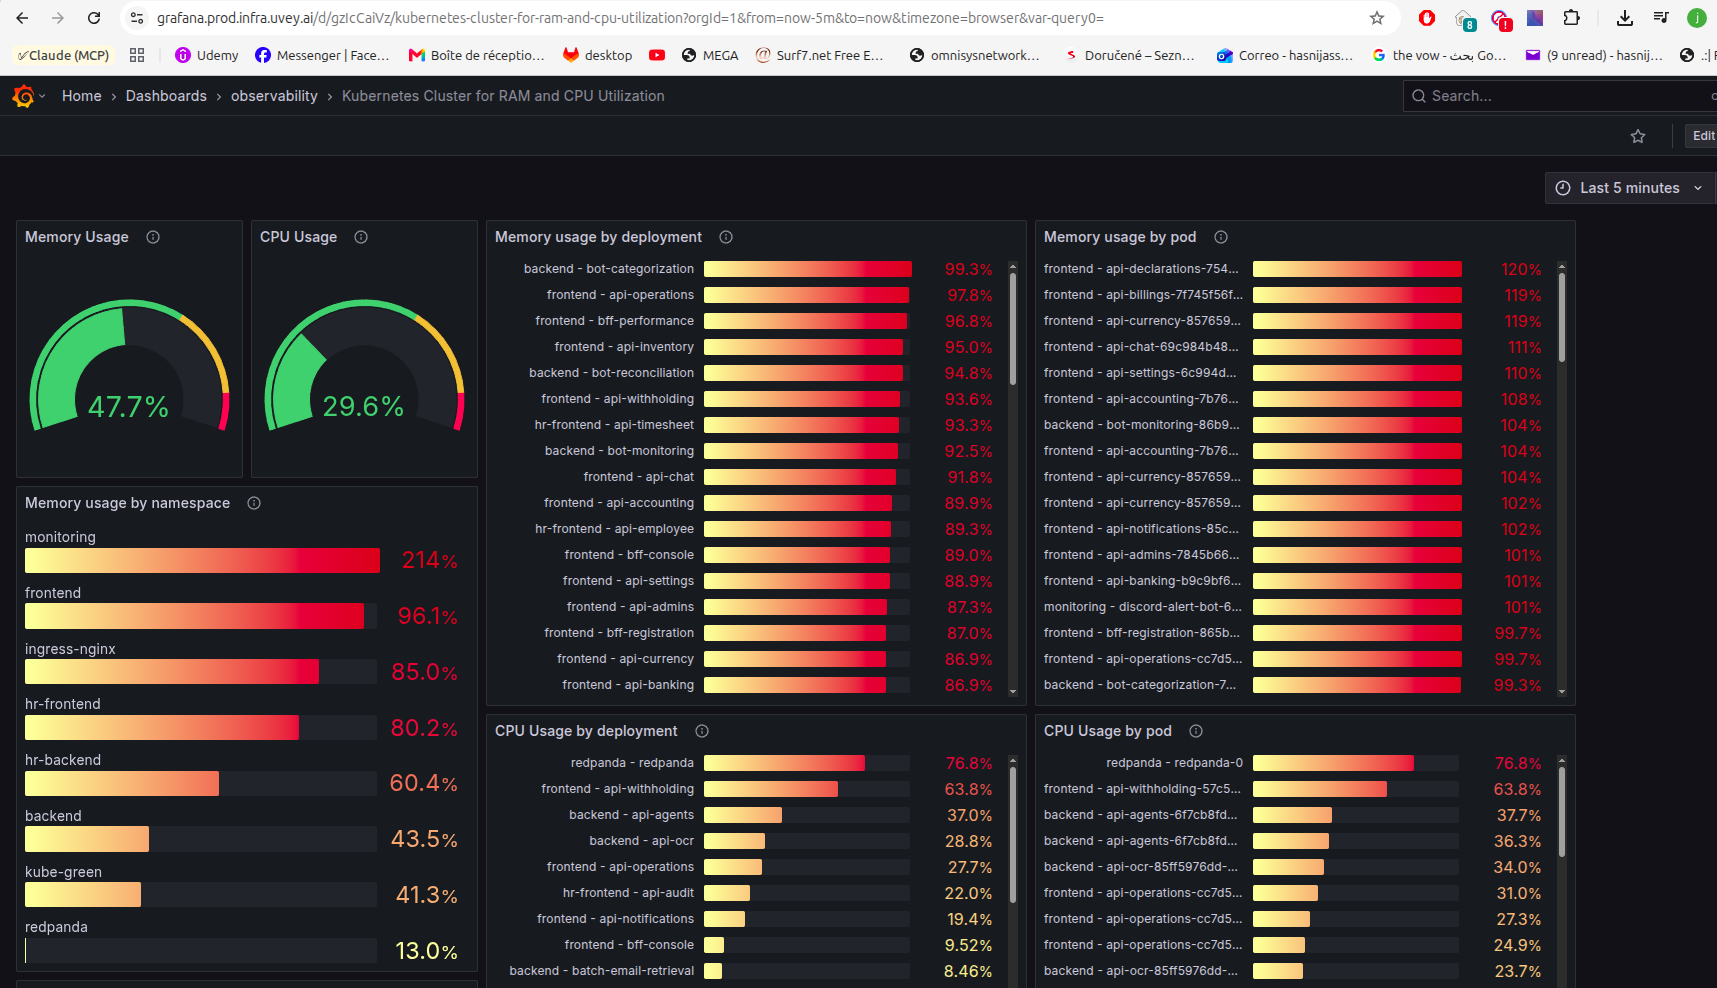
\includegraphics[width=\textwidth]{fig_grafana_dashboard}
  \caption{Tableau de bord Grafana --- métriques des microservices en production~\cite{prometheus2023docs}}
  \label{fig:grafana_dashboard}
\end{figure}

\begin{figure}[H]
  \centering
  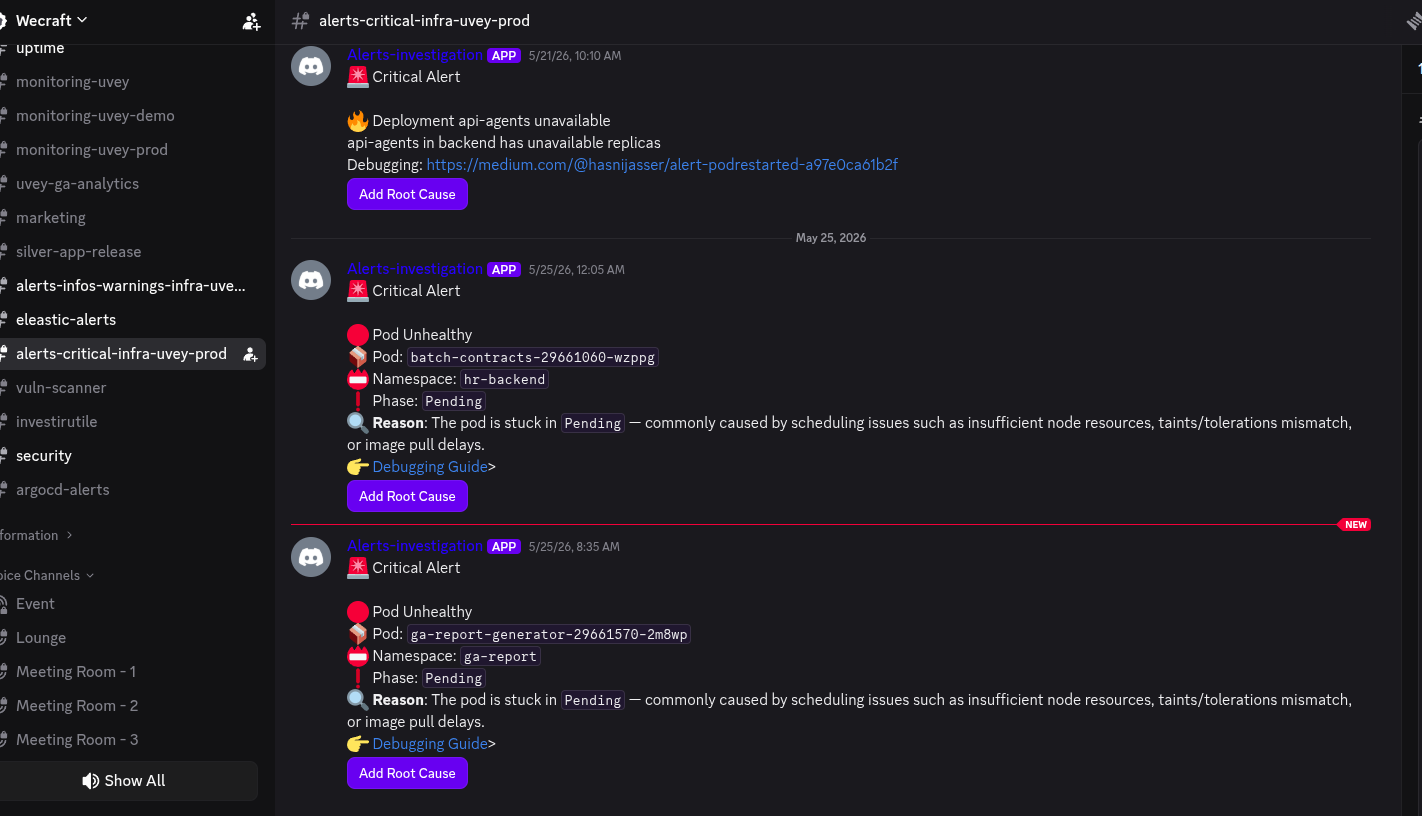
\includegraphics[width=0.92\textwidth]{fig_alertmanager}
  \caption{Configuration des alertes dans Alertmanager~\cite{prometheus2023docs}}
  \label{fig:alertmanager}
\end{figure}

\section{Traçage distribué avec OpenTelemetry}
\label{sec:tracing}

\noindent Cette section présente la mise en place du traçage distribué, en décrivant les choix d'instrumentation multi-langages et le flux de traitement des données de traces.

\subsection{Instrumentation multi-langages}

\noindent Dans un système composé de nombreux microservices implémentés en plusieurs langages de programmation, la solution \tech{OpenTelemetry}~\cite{opentelemetry2023docs} de la \ac{CNCF} a été retenue pour le traçage distribué. OpenTelemetry a été préféré aux solutions propriétaires pour sa neutralité vis-à-vis des fournisseurs : les traces générées par les \ac{SDK} OpenTelemetry peuvent être collectées par n'importe quel backend (Jaeger, Tempo, Zipkin ou Datadog) sans modification du code d'instrumentation, comme l'illustre le tableau~\ref{tab:otel_comparaison}.

\begin{table}[H]
  \centering
  \renewcommand{\arraystretch}{1.3}
  \begin{tabularx}{\textwidth}{L{4cm} C{3cm} C{3cm} C{3cm}}
    \toprule
    \rowcolor{uveylight}
    \textbf{Critère} & \textbf{OpenTelemetry} & \textbf{Jaeger SDK} & \textbf{Zipkin} \\
    \midrule
    Vendor-neutral       & Oui (\ac{CNCF})  & Non (Jaeger) & Non (Zipkin) \\
    Support multi-langages & Natif (10+) & Partiel & Partiel \\
    Logs + Métriques + Traces & Oui (unifié) & Traces seulement & Traces seulement \\
    Backend flexible     & Tout backend & Jaeger uniquement & Zipkin uniquement \\
    Standard industriel  & Oui (adopté \ac{CNCF}) & Non & Non \\
    \textbf{Choix}       & \textbf{Retenu} & Non retenu & Non retenu \\
    \bottomrule
  \end{tabularx}
  \caption{Comparaison des solutions de traçage distribué}
  \label{tab:otel_comparaison}
\end{table}

L'instrumentation s'effectue via les \ac{SDK} disponibles pour chaque langage (Node.js, Java, Go, Python, C\#), ce qui permet la propagation automatique du contexte de trace entre les différents services. Cette propagation automatique est un atout essentiel : sans elle, chaque service devrait relayer manuellement les identifiants de trace reçus dans ses communications entrantes vers ses appels sortants, augmentant considérablement la complexité de mise en œuvre. La Figure~\ref{fig:distributed_tracing} illustre le parcours complet d'une requête traversant plusieurs microservices, en faisant apparaître la décomposition en \textit{spans} imbriqués, les durées de chaque appel et l'identification du composant introduisant la latence la plus élevée.

\begin{figure}[H]
  \centering
  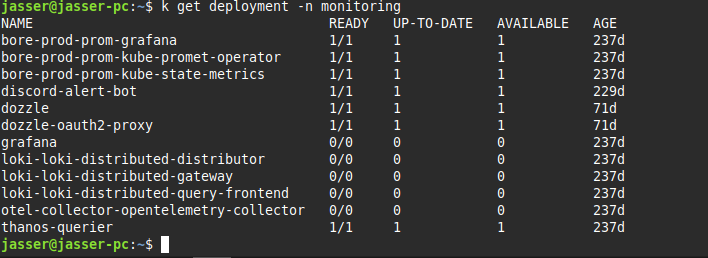
\includegraphics[width=\textwidth]{fig_distributed_tracing}
  \caption{Traçage distribué --- parcours d'une requête à travers les microservices~\cite{opentelemetry2023docs}}
  \label{fig:distributed_tracing}
\end{figure}

\subsection{Flux OpenTelemetry --- Agent Java vers les backends}

\noindent Le collector OpenTelemetry se connecte à la \ac{JVM} via l'option \texttt{-javaagent} dans le \texttt{Dockerfile} du microservice, ce qui permet de capturer automatiquement les traces, métriques et logs d'un service Spring Boot sans modifier une seule ligne du code applicatif. Ce principe d'instrumentation par agent présente un avantage majeur pour l'adoption : les développeurs n'ont pas besoin d'instrumenter manuellement leurs applications ni d'ajouter des dépendances dans leurs fichiers de build. L'agent intercepte automatiquement les appels aux frameworks et bibliothèques couramment utilisés (Spring Web, JDBC, Redis, Kafka) et produit les \textit{spans} permettant d'obtenir une trace complète du parcours d'une requête.

Ces données sont ensuite transmises vers l'OpenTelemetry Collector, qui les achemine vers les backends appropriés pour chaque type de signal : Tempo ou Jaeger pour les traces, Prometheus pour les métriques, et Elasticsearch pour les logs structurés. L'OpenTelemetry Collector constitue le point clé de cette architecture car il découple les \ac{SDK} d'instrumentation des backends d'ingestion : si l'organisation décide de passer de Jaeger à Tempo, seule la configuration du Collector doit être mise à jour. La Figure~\ref{fig:otel_config} représente ce flux de bout en bout, depuis l'agent Java attaché à la JVM jusqu'au routage des signaux vers Tempo, Prometheus et Elasticsearch par le Collector, illustrant comment un seul point de configuration central gouverne l'ensemble de la chaîne d'observabilité.

\begin{figure}[H]
  \centering
  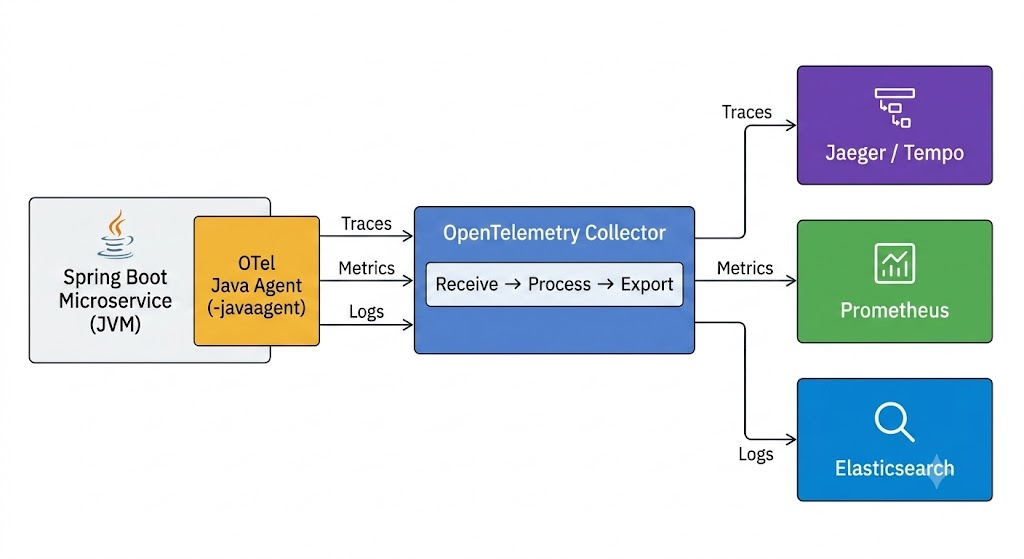
\includegraphics[width=\textwidth]{fig_otel_config}
  \caption{Flux OpenTelemetry --- de l'agent Java au Collector et aux backends~\cite{opentelemetry2023docs}}
  \label{fig:otel_config}
\end{figure}

\section{Intégration de l'observabilité dans l'IDP}
\label{sec:obs_idp}

La pile d'observabilité complète est interconnectée avec l'\ac{IDP}. Grâce au \textit{Software Catalog}, chaque développeur peut accéder instantanément à l'état de santé de ses microservices via des liens profonds pré-filtrés et pré-configurés vers les outils Grafana, Kibana et Jaeger/Tempo. Sans cette intégration, un développeur confronté à une alerte devrait connaître les URLs de chacun de ces outils, naviguer vers le bon tableau de bord et appliquer les bons filtres pour visualiser les données pertinentes --- un processus inutilement long et source d'erreurs sous pression. Grâce à l'intégration au sein de l'\ac{IDP}, un simple clic depuis la fiche de service amène directement au bon tableau de bord, sans que le développeur n'ait à maîtriser l'ensemble de ces outils.

Cette intégration apporte plusieurs bénéfices concrets :
\begin{itemize}[itemsep=0.15cm, topsep=0.2cm]
  \item \textbf{Réduction du \ac{MTTR} :} accès direct aux logs, métriques et traces filtrés par service depuis une interface unique, sans navigation manuelle entre les outils.
  \item \textbf{Corrélation des données :} possibilité de corréler une alerte Grafana avec les logs Kibana et les traces OpenTelemetry correspondants, en suivant la chronologie d'un incident à travers les trois piliers.
  \item \textbf{Élimination du \textit{context switching} :} les développeurs n'ont plus besoin de naviguer entre quatre interfaces distinctes pour diagnostiquer un incident, ce qui réduit la charge cognitive et le risque d'erreur sous pression.
  \item \textbf{Démocratisation de l'observabilité :} les développeurs moins expérimentés peuvent accéder aux données de leur service sans formation préalable sur chaque outil.
\end{itemize}

\section*{Conclusion}
\addcontentsline{toc}{section}{Conclusion}

\noindent Ce chapitre a détaillé les différentes étapes de mise en place de la pile d'observabilité complète, transformant l'architecture d'Uvey en une architecture pleinement observable. Les trois piliers fondamentaux ont chacun été analysés : la centralisation de la collecte des logs via la stack ELK avec Fluent-bit en DaemonSet, retenu pour sa faible empreinte mémoire comparée à Fluentd ; le monitoring des métriques via Prometheus, choisi pour son intégration native Kubernetes et son écosystème \ac{CNCF}, ainsi que via Grafana avec des règles d'alertes versionnées dans Git ; et le traçage distribué via OpenTelemetry, distingué par sa neutralité vis-à-vis des fournisseurs et son support multi-langages natif, sans nécessiter de modification du code applicatif grâce à l'approche par agent. L'intégration de l'ensemble de ces solutions via des liens pré-filtrés par service dans l'\ac{IDP} transforme la plateforme en un véritable centre de contrôle opérationnel à destination de l'ensemble des équipes d'ingénierie.

\chapter*{Conclusion Générale et Perspectives}
\addcontentsline{toc}{chapter}{Conclusion Générale et Perspectives}
\label{chap:conclusion}

\noindent Ce projet de fin d'études a été réalisé chez la startup Uvey, en Tunisie. Il a
permis de concevoir, déployer et valider une solution répondant aux défis opérationnels
d'une équipe d'ingénierie gérant une architecture microservices en forte croissance. Au
delà d'une simple mise en œuvre de nouvelles technologies, ce projet a transfiguré les
pratiques de livraison logicielle et le mode opératoire en infrastructure de l'entreprise,
les rendant bien plus efficaces et reproductibles.

\medskip
\noindent Les objectifs du projet ont été totalement, ou pour le moins grandement,
atteints. Une infrastructure cloud-native sur Azure, répartie sur trois clusters \ac{AKS},
a été conçue et déployée via \textbf{Terraform}. Un pipeline \textbf{GitOps} complet a
été bâti, et une stack unifiée d'observabilité couvrant les logs, les métriques ainsi que
le tracing distribué a été mise en place. La migration de la base \textbf{PostgreSQL}
depuis \ac{GCP} vers Azure a été effectuée sans perte de données et sans interruption de
service. Un portail \textbf{Backstage} a été installé pour faciliter l'accès à l'ensemble
des outils de l'équipe.
\medskip

\noindent Ce projet a été un véritable apprentissage. La migration d'\textbf{Ingress NGINX}
vers \textbf{Application Gateway} avec \textbf{AGIC} a demandé de détailler les
annotations de chacun des microservices et de créer un environnement de test dédié. Lors
de la migration de \textbf{PostgreSQL}, des problèmes de compatibilité d'extensions entre
\textit{Cloud SQL} et \textit{Azure Flexible Server} ont nécessité des ajustements du
module \textbf{Terraform} avant de pouvoir reprendre le processus. Pour pallier aux
limitations de débit de l'API \textbf{ARM} d'Azure, nous sommes passés par un proxy
\textbf{Node.js} sur lequel nous avons implémenté un cache. D'un point de vue
organisationnel, la pratique de \textbf{Scrum} dans un contexte d'Infrastructure as Code
a révélé qu'il fallait prévoir des sprints avec plus de marge, ainsi qu'intégrer
explicitement la validation en environnement pré-prod dans la \textit{Definition of Done}.

\medskip
\noindent Pour dépasser ces challenges, nous sommes peu à peu convaincus qu'à ce jour,
aucune réussite sur du cloud public ne s'est affranchie de deux piliers fondamentaux~:
la \textbf{documentation architecturale} et l'\textbf{anticipation rigoureuse des
contraintes environnementales}. Ces deux dimensions sont tout aussi déterminantes que la
maîtrise technique pour réussir une transition vers le cloud.

%\bigskip

%\noindent \textbf{\large Perspectives :}

\medskip
\noindent Les travaux réalisés ouvrent plusieurs axes d'évolution naturels, structurés
autour de trois dimensions~:

\medskip
\noindent \textbf{Enrichissement de la plateforme développeur.} Le portail
\textbf{Backstage} pourrait être enrichi par l'intégration de \textit{scaffolders}
permettant aux équipes de provisionner elles-mêmes de nouveaux microservices conformes
aux standards architecturaux d'Uvey, réduisant ainsi davantage la friction entre
développement et infrastructure. Par ailleurs, l'adoption de \textbf{Karpenter} en
remplacement du \textit{Cluster Autoscaler} d'Azure permettrait un provisionnement des
n\oe{}uds \ac{AKS} plus réactif et économiquement optimisé, notamment grâce à la gestion
des instances Spot.

\medskip
\noindent \textbf{Renforcement de la sécurité et de l'observabilité.} Le déploiement
d'une stratégie réseau de type \textbf{zero-trust} avec \textbf{Cilium} ou \textbf{Azure
Network Policy} serait un prolongement naturel de l'existant avec \textit{Managed
Identity}, en allant jusqu'à contrôler chaque interconnexion entre les différents services
au sein des clusters. Du point de vue de l'observabilité, la généralisation du tracing
distribué vers un modèle \textbf{eBPF} permettrait de capter des signaux de performance
de manière non-intrusive, offrant une visibilité complète sur les échanges réseau
sous-jacents.

\medskip
\noindent \textbf{Conformité et certification.} À terme, la maturité de la plateforme
ouvrira la possibilité de viser une certification \textbf{ISO 27001} ou une attestation
\textbf{SOC 2}, des labels recherchés par les FinTechs pour médiatiser leur confiance
auprès de clients B2B et accélérer leur processus de vente sur des marchés régulés.

%% ---
\addcontentsline{toc}{chapter}{Bibliographie}
\bibliographystyle{unsrtnat}
\bibliography{references}

\end{document}
